\begin{chapterpage}{Inference for categorical data}
  \chaptertitle{Inference for categorical data}
  \label{inferenceForCategoricalData}
  \label{ch_inference_for_props}
  \chaptersection{singleProportion}
  \chaptersection{differenceOfTwoProportions}
  \chaptersection{oneWayChiSquare}
  \chaptersection{twoWayTablesAndChiSquare}
\end{chapterpage}
\renewcommand{\chapterfolder}{ch_inference_for_props}

\chapterintro{In this chapter,
we apply the methods and ideas from Chapter~\ref{ch_foundations_for_inf}
in several contexts for categorical data.
We'll start by revisiting what we learned for a single
proportion, where a normal distribution can be used
to model the uncertainty in the sample proportion.
Next, we apply these same ideas to analyze the difference of two proportions using a normal model.
Later in the chapter we will encounter contingency tables,
and we will use a different distribution, though the core
ideas of hypothesis testing remain the same.}



%____________________________________
\section[Inference for a single proportion]{Inference for a single proportion }
\label{singleProportion}

\sectionintro{
\noindent%
In this section, we will apply the inferential procedures introduced in Chapter~\ref{ch_foundations_for_inf} to the context of a single proportion, and we will explore how to do sample~size calculations for data collection purposes.
We will answer questions such as the following:
\begin{itemize}
\item Do greater than half of adults in the U.S. oppose nuclear energy?
\item What percent of adults in the U.S. approve of the way the Supreme Court is handling its job?
\item
    What is the standard error is associated with
    this estimate?  
\item
    How do we construct a confidence interval for this value?
\item
    What sample~size is required to estimate this within a 3\%
    margin of error using a 95\% confidence level?

\end{itemize}


%%
\subsection*{Learning objectives}
\begin{enumerate}
\setlength{\itemsep}{0mm}
\item State and verify whether or not the conditions for inference on a proportion using a normal distribution are met.

\item Recognize that the success-failure condition and the standard error calculation are different for the test and for the confidence interval and explain why this is the case.

\item Carry out a complete hypothesis test and confidence interval procedure for a single proportion.

\item Find the minimum sample~size needed to estimate a proportion with C\% confidence and a margin of error no greater than a certain value.

\item Recognize that margin of error calculations only measure sampling error, and that other types of errors may be present.

\end{enumerate}
}


\D{\newpage}

%%
\subsection{Distribution of a sample proportion (review)}

The distribution of a sample proportion, such as the distribution of all possible values for the proportion of people who share a particular opinion in a poll, was introduced in Section~\ref{distributionphat}.  When the sampling distribution for a sample proportion, $\hat{p}$, is approximately normal, we can use confidence intervals and hypothesis tests based on a normal distribution.  We call these Z-intervals and Z-tests for short.  Here, we review the conditions necessary for a sample proportion to be modeled using a normal distribution.

\begin{onebox}{Conditions for the sampling distribution for \pmb{$\hat{{p}}$} being nearly normal}
The sampling distribution for a sample proportion, $\hat{p}$, based on a random sample of size $n$ from a population with a true proportion $p$, is nearly normal when
\begin{enumerate}
\item the sample observations are independent and
\item $np\geq10$ and $n(1-p)\geq10$. This is called the \term{success-failure condition}.
\end{enumerate}
If these conditions are met, then the sampling distribution for $\hat{p}$ is nearly normal with mean $\mu_{\hat{p}}=p$ and standard deviation $\sigma_{\hat{p}} = \sqrt{\frac{\ p(1-p)\ }{n}}$.\index{standard error!single proportion}\end{onebox}

\subsection{Checking conditions for inference using a normal distribution}
We can use a normal model for inference for a proportion when the \textbf{sampling distribution for the sample proportion is nearly normal}.  We check that this assumption is reasonable by assessing the independence assumption and verifying that the success-failure condition is met. 

\begin{description}
\setlength{\itemsep}{0mm}
\item[Independence.] Observations can be considered independent when the data are collected from a \emph{random process}, such as tossing a coin, or from a \emph{random sample}.  Without a random sample or process, the standard error formula would not apply, and it is unclear to what population the inference would apply.  When sampling without replacement from a finite population, the observations can be considered independent when sampling less than 10\% of the population.\footnote{When sampling without replacement and sampling greater than 10\% of the population, a modified standard error formula should be used.}
\item[Success-failure condition.] We saw in Section~\ref{distributionphat} that, when that the observations are independent, the sampling distribution for a sample proportion will be nearly normal if the success-failure condition is met, i.e. when the expected number of successes and failures are both at least 10.  
\end{description}


\D{\newpage}

%%
\subsection{Confidence intervals for a proportion}
\label{confIntForPropSection}

\index{data!supreme court|(}
\index{point estimate!single proportion}
\index{Z-interval!for a proportion|(}

The Gallup organization began measuring the public's view of the Supreme Court's job performance in 2000, and has measured it every year since then with the question: ``Do you approve or disapprove of the way the Supreme Court is handling its job?".  In 2018, the Gallup poll randomly sampled 1,033 adults in the U.S. and found that 53\% of them approved.\footnote{\oiRedirect{textbook-gallup_supreme_court_approval_2018}{\scriptsize https://news.gallup.com/poll/237269/supreme-court-approval-highest-2009.aspx}}  We know that 53\% is just a point estimate.  What range of values are reasonable estimates for the percent of the population that approved of the job the Supreme Court is doing?  We can use the confidence interval procedure introduced in the previous chapter to answer this question, but first we must clearly identify the parameter we're trying to estimate and be sure that a Z-interval will be appropriate.  The following examples walk through the various steps for carrying out a confidence interval procedure using the Gallup poll data.

\begin{examplewrap}
\begin{nexample}{Identify the population of interest and the parameter of interest for the Gallup poll about the U.S. Supreme Court. }
Gallup sampled from U.S. adults, therefore the population of interest, and the population to which we can make an inference, is U.S. adults.  We know the percent of the sample that said they approve of the job the Supreme Court is doing.  However, we do not know what percent of the population would approve.  The parameter of interest, which is unknown, is the percent of \emph{all} U.S. adults that approve of the job the Supreme Court is doing.  This is the quantity that we seek to estimate with the confidence interval.
\end{nexample}
\end{examplewrap}


\begin{examplewrap}
\begin{nexample}{Can the sample proportion $\hat{p}$ be modeled using a normal distribution?}
In order to construct a Z-interval, the sample statistic must be able to be modeled using a normal distribution.  Gallup took a random sample of adults in the U.S.  The sample is random and the sample size is much less than 10\% of the population size, so the first condition (the independence condition) is satisfied.  We must also test the second condition (the success-failure condition) to ensure that the sample~size is large enough for the central limit theorem to apply.  The success-failure condition is met when $np$ and $n(1-p)$ are at least 10. Since $p$ is always unknown when constructing a confidence interval for $p$, we use the sample proportion $\hat{p}$ to check this condition.  Here we have:
\begin{align*}
n\hat{p} = 1033(0.53) = 547\text{ (``successes'')} \\
 n(1-\hat{p}) = 1033(1 - 0.53) = 486\text{ (``failures'')}
\end{align*}
The second condition is satisfied since 547 and 486 are both at least 10. With the two conditions satisfied, we can model the sample proportion $\hat{p}$ using a normal model and we can construct a Z-interval.
\end{nexample}
\end{examplewrap}

\D{\newpage}

\begin{examplewrap}
\begin{nexample}{Calculate the point estimate and the $SE$ of the estimate.}
\label{supremeCourtCISEExample}
The point estimate for the unknown parameter $p$ (the proportion of all U.S. adults) who approve of the job the Supreme Court is doing) is the sample proportion. The point estimate here is $\hat{p} = 0.53$.

Because the point estimate is the sample proportion, the $SE$ of the estimate is the $SE$ of $\hat{p}$.  
In Section~\ref{distributionphat}, we learned that the formula for the standard deviation of $\hat{p}$ is
\begin{align*}
\sigma_{\hat{p}} = \sqrt{\frac{\ p(1-p)\ }{n}}
\end{align*}
The proportion $p$ is unknown, so we use the sample proportion $\hat{p}$ to find the $SE$ of $\hat{p}$.  
\begin{align*}
SE = \sqrt{\frac{\ \hat{p}(1-\hat{p})\ }{n}}
\end{align*}

Here $\hat{p}=0.53$ and $n=1,033$, so the $SE$ of the sample proportion is:
\begin{align*}
SE = \sqrt{\frac{\ 0.53(1-0.53)\ }{1033}}=0.016
\end{align*}
\end{nexample}
\end{examplewrap}


\begin{examplewrap}
\begin{nexample}{Construct a 90\% confidence interval for $p$, the proportion of all U.S. adults that approve of the job the Supreme Court is doing.}
\label{90CIForJobSupremeCourtDoingExample}
Recall that the general form of a confidence interval is:
\begin{align*}
\text{point estimate}\ \pm\ \text{critical value} \times SE\ \text{of estimate}\vspace{-2mm}
\end{align*}
We have already found the point estimate and the $SE$ of the estimate.  Because we previously verified that $\hat{p}$ can be modeled using a normal distribution, the critical value is a $z^{\star}$.  The $z^{\star}$ value can be found in the $t$-table on page~\pageref{tDistributionTable}, using the bottom row ($\infty$), where the column corresponds to the confidence level.  Here the confidence level is 90\%, so  $z^{\star}$=1.65.  We can now construct the 90\% confidence interval as follows.  
\begin{align*}
\text{point estimate}\ \pm&\  z^{\star} \times SE\ \text{of estimate} \\
0.53\ \pm&\  1.65 \times 0.016 \\
= (0.5&04,\ 0.556)
\end{align*}
We are 90\% confident that the true proportion of U.S. adults who approve of the job the Supreme Court is doing is between 0.504 and .556. 
\end{nexample}
\end{examplewrap}


\begin{examplewrap}
\begin{nexample}{Based on the interval, is there evidence that more than half of U.S. adults approve of the job the Supreme Court is doing?}
\label{JobSupremeCourtDoingEvidenceExample}
The 90\% confidence interval (0.504,\ 0.556) provides an interval of reasonable values for the parameter.  The value 0.50 is not in the interval, therefore can be considered unreasonable.  Because the \emph{entire} interval is above 0.50, we do have evidence, at the 90\% confidence level, that more than half of U.S. adults (at the time of this poll) approve of the job the Supreme Court is doing.
\end{nexample}
\end{examplewrap}

\begin{examplewrap}
\begin{nexample}{Do we have evidence at the 95\% confidence level that more than half of U.S. adults approve of the job the Supreme Court is doing?}
\label{JobSupremeCourtDoingWrapUpExample}
First, we observe that a 95\% confidence interval will be \emph{wider} than a 90\% confidence interval.  For a 95\% Z-interval, $z^{\star}=1.96$.  The 95\% confidence interval is:
\begin{align*}
&0.53\ \pm\  1.96 \times 0.016 \\
&= (0.499,\ 0.561)
\end{align*}
Now, we see that 0.50 is just barely inside the interval, making it within the range of reasonable values.  Therefore, we do not have evidence, at the 95\% confidence level, that more than half of U.S. adults (at the time of this poll) approve of the job the Supreme Court is doing.

Notice that we come to a different conclusion based on different confidence levels, which may feel a little jarring.  However, this will happen with real data, and it highlights why it is important to be explicit in identifying the confidence level being used.
\end{nexample}
\end{examplewrap}


Having worked through this example, we now summarize the steps for constructing a confidence interval for a proportion using the five step framework introduce in Chapter 5.

%~\ref{foundationsForInference}.

\begin{onebox}{Constructing a confidence interval for a proportion}
To carry out a complete confidence interval procedure to estimate a single proportion $p$,
\\
\\
\inferencestep{Identify} Identify the parameter and the confidence level, C\%. \vspace{-1mm}
\begin{itemize} 
\item[] The parameter will be a population proportion, e.g. the proportion of all U.S. adults that approve of the job the Supreme Court is doing.
\end{itemize}
\inferencestep{Choose} Choose the correct interval procedure and identify it by name. \vspace{-1mm}
\begin{itemize} 
\item[] To estimate a single proportion we use a \termsub{1-proportion Z-interval}{Z-interval!for a proportion}.
\end{itemize}
\inferencestep{Check} Check conditions for the sampling distribution for $\hat{p}$ to be nearly normal.  \vspace{-1mm}
\begin{itemize}
\setlength{\itemsep}{0mm}
\item[] 1. Independence:  Data come from a random sample or random process.  When sampling 
\item[] \quad \ without replacement, check that sample size is less than 10\% of the population size.
\item[] 2. Success-failure:  $n\hat{p}\ge 10$ and $n(1-\hat{p})\ge 10$.
\end{itemize}
\inferencestep{Calculate} Calculate the confidence interval and record it in interval form.
\begin{itemize}
\item[] $\text{point estimate}\ \pm\ z^{\star} \times SE\ \text{of estimate}$
\begin{itemize}
\item[] point estimate: the sample proportion $\hat{p}$
\item[] $SE$ of estimate:  $\sqrt{\frac{\ \hat{p}(1-\hat{p})\ }{n}}$
\item[] $z^{\star}$: use a $t$-table at row $\infty$ and confidence level C\%
\end{itemize}
\item[] (\underline{\ \ \ \ \ }, \underline{\ \ \ \ \ })
\end{itemize}
\inferencestep{Conclude} Interpret the interval and, if applicable, draw a conclusion in context.\vspace{-1mm}
\begin{itemize}
\item[] We are C\%  confident that the true \emph{proportion} of [...] is between \underline{\ \ \ \ \ } and  \underline{\ \ \ \ \ }. If applicable, draw a conclusion based on whether the interval is entirely above, is entirely below, or contains the value of interest. 
\end{itemize}\end{onebox}


\begin{examplewrap}
\begin{nexample}
{A February 2018 Marist Poll reports:  ``Many Americans (68\%) think there is intelligent life on other planets."\footnotemark\,  The results were based on a random sample of 1,033 adults in the U.S.  Does this poll provide evidence at the 95\% confidence level that greater than half of all U.S. adults think there is intelligent life on other planets?  Carry out a confidence interval procedure to answer this question.  Use the five step framework to organize your work.  
}
\label{IntelligentLife}
\begin{description}
\item[\inferencestep{Identify}] First we identify the parameter of interest.  Here the parameter is the true proportion of U.S. adults that think there is intelligent life on other planets.  We will estimate this at the 95\% confidence level.  
\item[\inferencestep{Choose}] Because the parameter to be estimated is a single proportion, we will use a 1-proportion Z-interval.
\item[\inferencestep{Check}] We must check that a Z-interval is appropriate.    The problem states that the data come from a random sample, and since the population is adults in the U.S., the population size is much more than 10 times larger than the sample size.  Next we must check the success-failure condition.  Here, we have that $1033(.68)\ge 10$ and $1033(1-0.68)\ge 10$.  The nearly normal sampling distribution conditions are met, so we can proceed with a 1-proportion Z-interval.
\item[\inferencestep{Calculate}]  We will calculate the interval:
\begin{align*}
 \text{point estimate}\ \pm\ z^{\star} \times SE\ \text{of estimate}
\end{align*}
The point estimate is the sample proportion:  $\hat{p} = 0.68$\\
\\ 
The $SE$ of the sample proportion is:  $\sqrt{\frac{\ \hat{p}(1-\hat{p})\ }{n}} = \sqrt{\frac{0.68(1-0.68)}{1033}}=0.015$.\\
\\
$z^{\star}$ is found using the $t$-table at row $\infty$ and confidence level C\%.  \\
For a 95\% confidence level, $z^{\star}$ = 1.96. \\

The 95\% confidence interval is given by:
\begin{align*}
0.68\ \pm\  &1.96 \times \sqrt{\frac{0.68(1-0.68)}{1033}} \\
0.68\ \pm\  &1.96 \times 0.015 \\
 = (0.6&51,\  0.709)
\end{align*}
\item[\inferencestep{Conclude}]  We are 95\%  confident that the true \emph{proportion} of U.S. adults that think there is intelligent life on other planets is between 0.651 and 0.709. Because the entire interval is above 0.5 we have evidence that greater than half of all U.S. adults think there is intelligent life on other planets.
\end{description}
\end{nexample}
\end{examplewrap}
\footnotetext{This estimate of 68\% in 2018 was up from an estimate of 52\% in 2005. \oiRedirect{textbook-intelligent_life_2018}{http://maristpoll.marist.edu/212-are-americans-poised-for-an-alien-invasion}}

\begin{exercisewrap}
\begin{nexercise}
True or False:  There is a 95\% probability that between 65.1\% and 70.9\% of U.S. adults think that there is intelligent life on other planets.\footnotemark
\end{nexercise}
\end{exercisewrap}
\footnotetext{False.  The true percent of U.S. adults that think there is intelligent life on other planets either falls in that interval or it doesn't.  A correct interpretation of the confidence level would be that if we were to repeat this process over and over, about 95\% of the 95\% confidence intervals constructed would contain the true value.  }


\D{\newpage}

%%
\subsection{Calculator:  the 1-proportion Z-interval}
A calculator can be helpful for evaluating the final interval in the Calculate step.  However, it should not be used as a substitute for understanding.  
\label{1PropZInt}

\begin{onebox}{\videohref{ti84_1_prop_CI} TI-83/84: 1-proportion Z-interval}
Use \calcbutton{STAT}, \calctext{TESTS}, \calctext{1-PropZInt}.
\begin{enumerate}
\setlength{\itemsep}{0mm}
\item Choose \calcbutton{STAT}.
\item Right arrow to \calctext{TESTS}.
\item Down arrow and choose \calctext{A:1-PropZInt}.
\item Let \calctext{x} be the \emph{number} of yeses (must be an integer).
\item Let \calctext{n} be the sample~size.
\item Let \calctext{C-Level} be the desired confidence level.
\item Choose \calctext{Calculate} and hit \calcbutton{ENTER}, which returns\\[1mm]
\begin{tabular}{l l}
\calctext{(\underline{\ \ },\underline{\ \ })} & the confidence interval \\
$\calctextmath{\hat{p}}$ & the sample proportion \\
\calctext{n} & the sample~size
\end{tabular}
\end{enumerate}
\end{onebox}

\begin{onebox}{\videohref{casio_1_prop_inference} Casio fx-9750GII: 1-proportion Z-interval}
% Quick navigation: \calctext{STAT} (via \calcbutton{MENU} button), \calctext{INTR}, \calctext{Z}, and \calctext{1-P}.
\begin{enumerate}
\setlength{\itemsep}{0mm}
\item Navigate to \calctext{STAT} (\calcbutton{MENU} button, then hit the \calcbutton{2} button or select \calctext{STAT}).
\item Choose the \calctext{INTR} option (\calcbutton{F4} button).
\item Choose the \calctext{Z} option (\calcbutton{F1} button).
\item Choose the \calctext{1-P} option (\calcbutton{F3} button).
\item Specify the interval details:\vspace{-1.5mm}
  \begin{itemize}
  \setlength{\itemsep}{0mm}
  \item Confidence level of interest for \calctext{C-Level}.
  \item Enter the number of successes, \calctext{x}.
  \item Enter the sample~size, \calctext{n}.
  \end{itemize}
\item Hit the \calcbutton{EXE} button, which returns \\[1mm]
  \begin{tabular}{ll}
  \calctext{Left}, \calctext{Right} & ends of the confidence interval \\
  $\calctextmath{\hat{p}}$ & sample proportion \\
  \calctext{n} & sample~size
  \end{tabular}
\end{enumerate}
\end{onebox}

\begin{exercisewrap}
\begin{nexercise}
Using a calculator, evaluate the confidence interval from Example~\ref{IntelligentLife}.  Recall that we wanted to find a 95\% confidence interval for the proportion of U.S. adults who think there is intelligent life on other planets.  The sample percent was 68\% and the sample~size was 1,033.\footnotemark
\end{nexercise}
\end{exercisewrap}
\footnotetext{Navigate to the 1-proportion Z-interval on the calculator.  To find \calctext{x}, the number of yes responses in the sample, we multiply the sample proportion by the sample~size.  Here $0.68\times 1033=702.44$.  We must round this to an integer, so we use \calctext{x} = 702.  Also, \calctext{n} =1033 and \calctext{C-Level} = 0.95.  The calculator output of (0.651, 0.708) matches our previously computed interval of (0.651, 0.709) with minor rounding difference.}

\index{Z-interval!for a proportion|)}

\D{\newpage}

%%
\subsection{Choosing a sample~size when estimating a proportion}
\label{moeproportion}
\index{margin of error|(}

Planning a sample~size before collecting data is important. If we collect too little data, the standard error of our point estimate may be so large that the estimate is not very useful. On the other hand, collecting data in some contexts is time-consuming and expensive, so we don't want to waste resources on collecting more data than we need.

When considering the sample~size, we want to put an upper bound on the margin of error. Recall that the \term{margin of error} is measured as the distance between the point estimate and the lower or upper bound of a confidence interval.  

\begin{onebox}{Margin of error}
The margin of error of a confidence interval is given by: 
\begin{align*}
\text{critical value} \ \times SE \text{ of estimate} 
\end{align*}
The margin of error for a C\% confidence interval tells us that we can be C\% confident that our point estimate is within that margin of error of the true value.  
\end{onebox}


\begin{examplewrap}
\begin{nexample}{Suppose we are conducting a university survey to determine whether students support a \$200 per year increase in fees to pay for a new football stadium.  Find the smallest sample~size $n$ so that the margin of error of the point estimate $\hat{p}$ will be no larger than 0.04 when using a 95\% confidence level.}
Because we are working with proportions, the critical value is a $z^{\star}$ value.  We want the margin of error to be less than or equal to 0.04, so we have:
\begin{align*}
z^{\star}\times \sqrt{\frac{p(1-p)}{n}} \leq 0.04
\end{align*}
There are two unknowns in the inequality: $p$ and $n$. If we have an estimate of $p$, perhaps from a similar survey, we could use that value. If we have no such estimate, we must use some other value for $p$. It turns out that the margin of error is largest when $p$ is 0.5, so we typically use this \emph{worst case estimate} of $p$ = 0.5 if no other estimate is available.
\begin{align*}
	1.96\times \sqrt{\frac{0.5(1-0.5)}{n}} &\leq 0.04 \\
	1.96^2\times \frac{0.5(1-0.5)}{n} &\leq 0.04^2 \\
	1.96^2\times \frac{0.5(1-0.5)}{0.04^2} &\leq n \\
	600.25 &\leq n \\
	n=601
\end{align*}
The sample~size must be an integer and we round up because $n$ must be greater than or equal to 600.25. We need at least 601 participants to ensure the sample proportion is within 0.04 of the true proportion with 95\% confidence.
\end{nexample}
\end{examplewrap}

No estimate of the true proportion is required in sample~size computations for a proportion. However, if we have a reliable estimate of the proportion, we should use it in place of the worst case estimate of~0.5.


\index{data!Congress approval rating|(}

 


\begin{examplewrap}
\begin{nexample}
{A recent estimate of Congress' approval rating was 17\%.\footnotemark\, If another poll were taken, what minimum sample~size does this estimate suggest should be used to have a margin of error no greater than 0.04 with 95\% confidence?}

We complete the same computations as before, except now we use $0.17$ instead of $0.5$ for $p$:
\begin{align*}
1.96\times \sqrt{\frac{0.17(1-0.17)}{n}} &\leq 0.04\\
n &\geq 338.8\\
n &= 339
\end{align*}
If the true proportion is 0.17, then 339 is the minimum sample~size that will ensure a margin of error no greater than 0.04 with 95\% confidence.

\index{data!Congress approval rating|)}

\end{nexample}
\end{examplewrap}
\footnotetext{\oiRedirect{textbook-gallup_congress_2018}{news.gallup.com/poll/237176/snapshot-congressional-job-approval-july.aspx}}

\begin{onebox}{Identify a sample~size for a particular margin of error}
When estimating a single proportion, we find the minimum sample~size $n$ needed to achieve a margin of error no greater than $m$ with a specified confidence level as follows:
\begin{align*}
z^{\star}\times \sqrt{\frac{p(1-p)}{n}} \leq m
\end{align*}
where $z^{\star}$ depends on the confidence level.   If no reliable estimate of $p$ exists, use $p = 0.5$.  	
\end{onebox}

\begin{exercisewrap}
\begin{nexercise}All other things being equal, what would we have to do to the sample size in order to halve the margin of error (decrease it by a factor of 2)?\footnotemark
\end{nexercise}
\end{exercisewrap}
\footnotetext{To decrease the error, we would need to increase the sample size.  We note that $\sqrt{n}$ is in the denominator of the $SE$ formula, so we would have to \emph{quadruple} the sample size in order to decrease the $SE$ by a factor of 2. The margin of error as well as the width of the confidence interval is proportional to $\frac{1}{\sqrt{n}}$.}

\begin{exercisewrap}
\begin{nexercise}
A manager is about to oversee the mass production of a new tire model in her factory, and she would like to estimate the proportion of these tires that will be rejected through quality control. The quality control team has previously found that about 6.2\% of tires fail inspection.
\begin{itemize}
\setlength{\itemsep}{0mm}
\item[(a)] How many tires should the manager examine to estimate the failure rate of the new tire model to within 2\% with a 90\% confidence level?\footnotemark
\item[(b)] What if the estimate of $p$ is 1.7\% rather than 6.2\%?\footnotemark
 
\index{margin of error|)}
\end{itemize}
\end{nexercise}
\end{exercisewrap}
\footnotetext{The $z^{\star}$ corresponding to a 90\% confidence level is 1.645.  Since we have an estimate for $p$ of 6.2\%, we use it.  So we have:  $1.645\times \sqrt{\frac{0.062(1-0.062)}{n}} \leq 0.02 $.  Rearranging for $n$ gives: $n \geq 393.4$, so she should use $n =394$.}
\footnotetext{Substituting 0.017 for $p$ gives an $n$ of 114.  We can note that in this case $n\times p = 114 \times 0.017 = 1.9 <10$.  Since the success-failure condition is not met, the use of $z^{\star} = 1.645$ based on a normal model is not appropriate.  We would need additional methods than what we've covered so far to get a good estimate for the minimum sample~size in this scenario.}



\D{\newpage}

%%
\subsection{Hypothesis testing for a proportion}
\label{htForPropSection}
\index{Z-test!for a proportion|(}

While a confidence interval provides a range of reasonable values for an unknown parameter, a hypothesis test evaluates a specific claim. In a hypothesis test, we set up competing hypotheses and find degrees of evidence against the null hypothesis.

\begin{examplewrap}
\begin{nexample}{Deborah Toohey is running for Congress, and her campaign manager claims she has more than 50\% support from the district's electorate. A newspaper collects a random sample of 500 likely voters in the district and estimates Toohey's support to be 52\%.
\begin{itemize}
%\item[(a)] What is the name of the test that is appropriate for this context?
\item[(a)] Identify the null and the alternative hypothesis. What value should we use as the null value, $p_{0}$?
\item[(b)] Can we model $\hat{p}$ using a normal model? Check the conditions.
\end{itemize}}
\label{TooheyTestNameAndConditionExample}
%(a) The name of the test we will use is the \emph{1-proportion Z-test}. \\[2mm]
(a) The alternative hypothesis, the one that bears the burden of proof, argues that Toohey has more than 50\% support. Therefore, $H_A$ will be one-sided and the null value will be $p_0 = 0.5$. So we have $H_0$: $p = 0.5$ and $H_A$: $p > 0.5$. Note that the hypotheses are about a population parameter.  The hypotheses are never about the sample.\\[2mm]
(b) First, we observe that the problem states that a random sample was chosen.  We assume that the size of the electorate in Toohey's district is more than 10 times the size of the sample.  Next, we check the success-failure condition.    Because we assume that $p = p_0$ for the calculations of the hypothesis test, we use the hypothesized value $p_0$ rather than the sample value $\hat{p}$ when verifying the success-failure condition.  
\begin{align*}
np_0 &\geq 10 \quad \rightarrow \quad 500(0.5) \geq 10 \\
n(1-p_0) &\geq 10 \quad \rightarrow \quad 500(1-0.5) \geq 10
\end{align*}
The conditions for a normal model are met.
\end{nexample}
\end{examplewrap}


In Chapter~\ref{foundationsForInference}, we saw that the general form of the test statistic for a hypothesis test takes the following form:
\begin{align*}
\text{test statistic} = \frac{\text{point estimate} - \text{null value}}{SE \text{ of estimate}}
\end{align*}
When the conditions for a normal model are met:
\begin{itemize}
\item We use Z as the test statistic and call the test a Z-test.
\item The point estimate is the sample proportion $\hat{p}$ (just like for a confidence interval).
\item Since we compute the test statistic assuming the null hypothesis (that $p = p_0$) is true, we compute the standard error of the sample proportion using the null value $p_0$.
\begin{align*}
SE = \sqrt{\frac{p_0(1-p_0)}{n}}
\end{align*}
\end{itemize}


\begin{onebox}{Confidence intervals versus hypothesis tests for a single proportion}
1-proportion Z-interval
\begin{align*}
\text{Check:}\quad n\hat{p}\ge 10 \text{ and }n(1-\hat{p})\ge 10 \qquad SE = \sqrt{\frac{\ \hat{p}(1-\hat{p})\ }{n}}
\end{align*}
1-proportion Z-test
\begin{align*}
\text{Check:}\quad  np_0\ge 10 \text{ and } n(1-p_0)\ge 10 \qquad SE = \sqrt{\frac{\ p_0(1-p_0)\ }{n}}
\end{align*}
\end{onebox}


\begin{examplewrap}
\begin{nexample}{(Continues previous example). Deborah Toohey's campaign manager claimed she has more than 50\% support from the district's electorate. A newspaper poll finds that 52\% of 500 likely voters who were sampled support Toohey. Does this provide convincing evidence for the claim by Toohey's manager at the 5\% significance level?}\label{TooheyInferenceExample}
We will use a one-sided test with the following hypotheses:
\begin{itemize}
\item[$H_0$:] $p = 0.5$. Toohey's support is 50\%.
\item[$H_A$:] $p > 0.5$. Toohey's manager is correct, and her support is higher than 50\%.
\end{itemize}
We will use a significance level of $\alpha = 0.05$ for the test. We can compute the standard error as
\begin{align*}
SE = \sqrt{\frac{\ p_0 (1 - p_0)\ }{n}} = \sqrt{\frac{\ 0.5 (1 - 0.5\ )}{500}} = 0.022
\end{align*}
The test statistic can be computed as:
\begin{align*}
Z =  \frac{\text{point estimate} - \text{null value}}{SE \text{ of estimate}} = \frac{0.52 - 0.50}{0.022} = 0.89
\end{align*}
Because the alternative hypothesis uses a greater than sign ($>$), this is an upper-tail test.  We find the area under the standard normal curve to the \emph{right} of $Z=0.89$.  A figure featuring the p-value is shown in Figure~\ref{pValueForCampaignManagerClaimOfMoreThan50PercentSupport} as the shaded region. 
\end{nexample}
\end{examplewrap}


\begin{figure}[h]
\centering
\Figure{.48}{pValueForCampaignManagerClaimOfMoreThan50PercentSupport}
\caption{Sampling distribution for the sample proportion if the null hypothesis is true for Example~\ref{TooheyInferenceExample}. The p-value for the test is shaded.}
\label{pValueForCampaignManagerClaimOfMoreThan50PercentSupport}
\end{figure}
Using a table or a calculator, we find the p-value is 0.19.  This p-value of 0.19 is greater than $\alpha = 0.05$, so we do not reject $H_0$. That is, we do not have sufficient  evidence to support Toohey's campaign manager's claims that she has more than 50\% support within the district.



\begin{examplewrap}
\begin{nexample}{Based on the result above, do we have evidence that Toohey's support equals 50\%?}
No.  In a hypothesis test we look for degrees of evidence \emph{against} the null hypothesis.  We cannot ever prove the null hypothesis directly.  The value 0.5 is reasonable, but many other values are reasonable as well.  There are many values that would not get rejected by this test.
\end{nexample}
\end{examplewrap}

We now summarize the steps for carrying out a hypothesis test for a proportion using the five step framework introduced in the previous chapter.

\begin{onebox}{Hypothesis testing for a proportion}
To carry out a complete hypothesis test to test the claim that a single proportion $p$ is equal to a null value $p_0$,
\\
\\
\inferencestep{Identify} Identify the hypotheses and the significance level, $\alpha$.\vspace{-1mm}
\begin{itemize}
\setlength{\itemsep}{0mm}
\item[] $H_0$: $p = p_0$  
\item[]  $H_A$: $p \ne p_0$;  \quad $H_A$: $p > p_0$; \quad or \quad $H_A$: $p < p_0$ 
\end{itemize} 
\inferencestep{Choose} Choose the correct test procedure and identify it by name.  \vspace{-1mm}
\begin{itemize}
\item[] To test hypotheses about a single proportion we use a \termsub{1-proportion Z-test}{Z-test!for a proportion}.
\end{itemize}
 \inferencestep{Check} Check conditions for the sampling distribution for $\hat{p}$ to be nearly normal, assuming $H_0$: $p=p_0$ is true.\vspace{-1mm}
\begin{itemize}
\setlength{\itemsep}{0mm}
\item[] 1. Independence:  Data come from a random sample or random process.  When sampling 
\item[] \quad \ without replacement, check that sample size is less than 10\% of the population size.
\item[] 2. Success-failure:  $np_0\ge 10$ and $n(1-p_0)\ge 10$
\end{itemize}
 \inferencestep{Calculate} Calculate the Z-statistic and p-value.
\begin{itemize}
\item[] $Z = \frac{\text{point estimate } - \text{ null value}}{SE \text{ of estimate}}$
\begin{itemize}
\item[] point estimate: the sample proportion $\hat{p}$
\item[] $SE$ of estimate:  $\sqrt{\frac{\ p_0(1-p_0)\ }{n}}$
\item[] null value: $p_0$
\end{itemize}
\item[] p-value = (based on the Z-statistic and the direction of $H_A$)
\end{itemize}
 \inferencestep{Conclude} Compare the p-value to $\alpha$, and draw a conclusion in context.  \vspace{-1mm}
\begin{itemize}
\item[] If the p-value is $< \alpha$, reject $H_0$; there is sufficient evidence that [$H_A$ in context]. 
\item[] If the p-value is $> \alpha$, do not reject $H_0$; there is not sufficient evidence that [$H_A$ in context].
\end{itemize}\end{onebox}


\begin{examplewrap}
\begin{nexample}
{A Gallup poll conducted in March of 2016 found that 54\% of respondents oppose nuclear energy.  This was the first time since Gallup first asked the question in 1994 that a majority of respondents said they oppose nuclear energy.\footnotemark\, The survey was based on telephone interviews from a random sample of 1,019 adults in the United States. Does this poll provide evidence that greater than half of U.S. adults oppose nuclear energy?  Carry out an appropriate test at the 0.10 significance level.  Use the five step framework to organize your work.  }
\label{NuclearEnergy}
\begin{description}
\item[\inferencestep{Identify}]  We will test the following hypotheses at the $\alpha=10\%$ significance level.\\
$H_0$: $p = 0.5$   \\
$H_A$: $p > 0.5$ \quad Greater than half of all U.S. adults oppose nuclear energy. \\
 
Note: $p>0.5$ is what we want to find evidence for; this bears the burden of proof, so this corresponds to $H_A$.
\item[\inferencestep{Choose}] Because the hypotheses are about a single proportion, we choose the 1-proportion Z-test.
\item[\inferencestep{Check}]  We must check the independence and success-failure conditions to show that the sample proportion can be modeled using a normal distribution.  The problem states that the data come from a random sample.  Again, the population is adults in the U.S., so the sample size is much smaller than 10\% of the population size.  Also, $1019(0.5)\geq10$ and $1019(1-0.5)\geq10$.  (Remember to use the hypothesized proportion, not the sample proportion, when checking the conditions for this test.)
\item[ \inferencestep{Calculate} ]  We will calculate the Z-statistic and the p-value.
\begin{align*}
Z = \frac{\text{point estimate } - \text{ null value}}{SE \text{ of estimate}}
\end{align*}

The point estimate is the sample proportion: $\hat{p} = 0.54.$\\
\\
The value hypothesized for the parameter in $H_0$ is the null value: $p_0 = 0.5$\\
\\
The $SE$ of the sample proportion, assuming $H_0$ is true, is: $\sqrt{\frac{p_0(1-p_0)}{n}}= \sqrt{\frac{0.5(1-0.5)}{1019}}$ \\
\begin{align*}
Z = \frac{0.54 - 0.5}{\sqrt{\frac{0.5(1-0.5)}{1019}}} = 2.5
\end{align*}
Because $H_A$ uses a greater than sign ($>$), meaning that it is an upper-tail test, the \mbox{p-value} is the area to the \emph{right} of $Z=2.5$ under the standard normal curve.  This area can be found using a normal table or a calculator.  The area or p-value = $0.006$.  
\item[\inferencestep{Conclude}]  The p-value of 0.006 is $< 0.10$, so we reject $H_0$; there is sufficient evidence that greater than half of U.S. adults oppose nuclear energy (as of March 2016).  
\end{description}
\end{nexample}
\end{examplewrap}
\footnotetext{\oiRedirect{textbook-nuclear_energy_support_2016}{www.gallup.com/poll/182180/support-nuclear-energy.aspx}} 



\begin{exercisewrap}
\begin{nexercise}
In context, interpret the p-value of 0.006 from the previous example.\footnotemark
\end{nexercise}
\end{exercisewrap}
\footnotetext{Assuming the normal model is accurate and assuming the null hypothesis is true, i.e. that the true proportion of U.S. adults that oppose nuclear energy really is 0.5, there is a 0.006 probability of getting a test statistic as large or larger than 2.5 ($H_0$ uses a $>$ sign, so the p-value is the area in the right tail).  Note: We start by assuming $H_0$ is true, that $p$ really equals 0.5.  Then, assuming this, we estimate the probability of getting a sample proportion of 0.54 or larger by finding the area under the standard normal curve to the right of 2.5.  This probability is very small, which casts doubt on the null hypothesis and leads us to reject it.  }


\D{\newpage}

%%
\subsection{Calculator:  the 1-proportion Z-test}
A calculator can be useful for evaluating the test statistic and computing the p-value.  
\label{1propZtest}

\begin{onebox}{\videohref{ti84_1_prop_HT} TI-83/84: 1-proportion Z-test}
Use \calcbutton{STAT}, \calctext{TESTS}, \calctext{1-PropZTest}.
\begin{enumerate}
\setlength{\itemsep}{0mm}
\item Choose \calcbutton{STAT}.
\item Right arrow to \calctext{TESTS}.
\item Down arrow and choose \calctext{5:1-PropZTest}.
\item Let $\calctextmath{p_0}$ be the null or hypothesized value of p.
\item Let \calctext{x} be the \emph{number} of yeses (must be an integer).
\item Let \calctext{n} be the sample~size.
\item Choose $\calctextmath{\ne}$, $\calctextmath{<}$, or $\calctextmath{>}$ to correspond to $H_A$.
\item Choose \calctext{Calculate} and hit \calcbutton{ENTER}, which returns \\[1mm]
\begin{tabular}{l l}
\calctext{z} & Z-statistic \\
\calctext{p} & p-value \\
$\calctextmath{\hat{p}}$ &  the sample proportion \\
\calctext{n} & the sample~size
\end{tabular}
\end{enumerate}
\end{onebox}


\begin{onebox}{\videohref{casio_1_prop_inference} Casio fx-9750GII: 1-proportion Z-test}
%Quick navigation: \calctext{STAT} (via \calcbutton{MENU} button), \calctext{TEST}, \calctext{Z}, and \calctext{1-P}.
The steps closely match those of the 1-proportion confidence interval.
\begin{enumerate}
\setlength{\itemsep}{0mm}
%\item Navigation is nearly the same as for the 1-proportion confidence interval: \\
\item Navigate to \calctext{STAT} (\calcbutton{MENU} button, then hit the \calcbutton{2} button or select \calctext{STAT}).
\item Choose the \calctext{TEST} option (\calcbutton{F3} button).
\item Choose the \calctext{Z} option (\calcbutton{F1} button).
\item Choose the \calctext{1-P} option (\calcbutton{F3} button).
%  navigate to \calctext{STAT} using the \calcbutton{MENU} button,
%  then go to \calctext{TEST} (instead of \calctext{INTR}),
%  choose \calctext{Z}, and
%  then choose \calctext{1-P}.
\item Specify the test details:
  \begin{itemize}
  \setlength{\itemsep}{0mm}
  \item Specify the sidedness of the test using the \calcbutton{F1}, \calcbutton{F2}, and \calcbutton{F3} keys.
  \item Enter the null value, \calctext{p0}.
  \item Enter the number of successes, \calctext{x}.
  \item Enter the sample~size, \calctext{n}.
  \end{itemize}
\item Hit the \calcbutton{EXE} button, which returns \\[1mm]
  \begin{tabular}{ll}
  \calctext{z} &  Z-statistic \\
  \calctext{p} &  p-value \\
  $\calctextmath{\hat{p}}$ &  the sample proportion \\
  \calctext{n} &  the sample~size
  \end{tabular}
\end{enumerate}
\end{onebox}

\begin{exercisewrap}
\begin{nexercise}
Using a calculator, find the test statistic and p-value for the earlier Example~\ref{NuclearEnergy}.  Recall that we were looking for evidence that more than half of U.S. adults oppose nuclear energy.  The sample percent was 54\%, and the sample~size was 1019.\footnotemark
\end{nexercise}
\end{exercisewrap}
\footnotetext{Navigate to the 1-proportion Z-test on the calculator.  Let $\calctextmath{p_0}$ = 0.5.  To find \calctext{x}, do $0.54\times 1019 = 550.26$. This needs to be an integer, so round to the closest integer.  Here \calctext{x} = 550.  Also, $\calctextmath{n}=1019$.  We are looking for evidence that greater than half oppose, so choose $\calctextmath{>p_0}$.  When we do \calctext{Calculate}, we get the test statistic: \calctext{Z = 2.64} and the p-value: \calctext{p = 0.006}. }

\index{Z-test!for a proportion|)}

\D{\newpage}

%%
\subsection*{Section summary}
\noindent Most of the confidence interval procedures and hypothesis tests of this book involve: a \term{point estimate}, the \term{standard error} of the point estimate, and an assumption about the \term{shape of the sampling distribution} of the point estimate. In this section, we explore inference when the parameter of interest is a \emph{proportion}.

\begin{itemize} 

\item We use the sample proportion $\hat{p}$ as the \emph{point estimate} for the unknown population proportion $p$. The sampling distribution for $\hat{p}$ is approximately normal when the success-failure condition is met and the observations are independent.  When the sampling distribution for $\hat{p}$ is normal, the standardized test statistic also follows a \term{normal} distribution.

\item When verifying the success-failure condition and calculating the $SE$, \vspace{-1mm}
\begin{itemize}
\setlength{\itemsep}{0mm}
\item use the \emph{sample} proportion $\hat{p}$ for the confidence interval, but 
\item use the \emph{null/hypothesized} proportion $p_0$ for the hypothesis test.
\end{itemize}

\item When there is one sample and the parameter of interest is a single proportion:\begin{itemize}
 \item Estimate $p$ at the C\% confidence level using a \termsub{1-proportion Z-interval}{Z-interval!for a proportion}.
\item Test $H_0$: $p=p_0$ at the $\alpha$ significance level using a \termsub{1-proportion Z-test}{Z-test!for a proportion}.
\end{itemize}

\item The one proportion Z-test and Z-interval require the sampling distribution for $\hat{p}$ to be nearly normal.  For this reason we must check that the following conditions are met.
\begin{itemize}
\item[1.] Independence:  The data should come from a random sample or random process.  When sampling without replacement, check that the sample size is less than 10\% of the population size.
\item[2.] Success-failure for Interval:  $n\hat{p}\ge 10$ and $n(1-\hat{p})\ge 10$.   \\\
Success-failure for Test, assuming $H_0$: $p=p_0$ is true: $np_0\ge 10$ and $n(1-p_0)\ge 10$.
\end{itemize}


\item When the conditions are met, we calculate the confidence interval and the test statistic as follows.
\begin{itemize}
\item[] Confidence interval:\ \  $\text{point estimate}\ \pm\ z^{\star} \times SE\ \text{of estimate}$
\item[] Test statistic: $Z = \frac{\text{point estimate } - \text{ null value}}{SE \text{ of estimate}}$ 
\end{itemize}
\item[] Here the point estimate is the sample proportion $\hat{p}$.
\item[] The $SE$ of estimate is the $SE$ of the sample proportion.  
\vspace{-1mm}
\begin{itemize}
\setlength{\itemsep}{0mm}
\item For an Interval, use $SE = \sqrt{\frac{\hat{p}(1-\hat{p})}{n}}$.
\item For a Test with $H_0$: $p=p_0$, use $SE = \sqrt{\frac{p_0(1-p_0)}{n}}$.
\end{itemize}

\item The \term{margin of error} ($ME$) for a one-sample confidence interval for a proportion is $z^{\star}\sqrt{\frac{\hat{p}(1-\hat{p})}{n}}$, which is proportional to $\frac{1}{\sqrt{n}}$.  

\item To find the \term{minimum sample~size} needed to estimate a proportion with a given confidence level and a given margin of error, $m$, set up an inequality of the form:
\begin{align*}
z^{\star}\sqrt{\frac{\hat{p}(1-\hat{p})}{n}}<m
\end{align*}
$z^{\star}$ depends on the desired confidence level.  Unless a particular proportion is given in the problem, use \mbox{$\hat{p}=0.5$.}  We solve for the sample~size $n$.  The final answer should be an \textit{integer}, since $n$ refers to a number of people or things.
\end{itemize}


%%%%%%%Section Exercises
{\exercisesheader{}

% 1 - orange_tabbies_CLT

\eoce{\qt{Orange tabbies\label{orange_tabbies_CLT}} Suppose that 90\% of orange
tabby cats are male. Determine if the following statements are true or false, 
and explain your reasoning.
\begin{parts}
\item The distribution of sample proportions of random samples of size 30 is 
left skewed.
\item Using a sample size that is 4 times as large will reduce the standard 
error of the sample proportion by one-half.
\item The distribution of sample proportions of random samples of size 140 is 
approximately normal.
\item The distribution of sample proportions of random samples of size 280 is 
approximately normal.
\end{parts}
}{}

% 2 - young_americans_CLT_2

\eoce{\qt{Young Americans, Part II\label{young_americans_CLT_2}} About 25\% of 
young Americans have delayed starting a family due to the continued economic 
slump. Determine if the following statements are true or false, and explain 
your reasoning.\footfullcite{news:youngAmericans2}
\begin{parts}
\item The distribution of sample proportions of young Americans who have 
delayed starting a family due to the continued economic slump in random 
samples of size 12 is right skewed.
\item In order for the distribution of sample proportions of young Americans 
who have delayed starting a family due to the continued economic slump to be 
approximately normal, we need random samples where the sample size is at 
least 40.
\item A random sample of 50 young Americans where 20\% have delayed starting 
a family due to the continued economic slump would be considered unusual.
\item A random sample of 150 young Americans where 20\% have delayed 
starting a family due to the continued economic slump would be considered 
unusual.
\item Tripling the sample size will reduce the standard error of the sample 
proportion by one-third.
\end{parts}
}{}

% 3 - gender_equality

\eoce{\qt{Gender equality\label{gender_equality}}
The General Social Survey asked a random sample of
1,390 Americans the following question:
``On the whole, do you think it should or should not be
the government's responsibility to  promote equality
between men and women?''
82\% of the respondents said it ``should be''.
At a 95\% confidence level, this sample has 2\% margin of error.
Based on this information, determine if the following statements
are true or false, and explain your reasoning.\footfullcite{data:gss}
\begin{parts}
\item We are 95\% confident that between 80\% and 84\% of Americans in this 
sample think it's the government's responsibility to promote equality between 
men and women.
\item We are 95\% confident that between 80\% and 84\% of all Americans 
think it's the government's responsibility to promote equality between 
men and women.
\item If we considered many random samples of 1,390 Americans, and we calculated 
95\% confidence intervals for each, 95\% of these intervals would include the 
true population proportion of Americans who think it's the government's 
responsibility to promote equality between men and women.
\item In order to decrease the margin of error to 1\%, we would need to 
quadruple (multiply by 4) the sample size.
\item Based on this confidence interval, there is sufficient evidence to 
conclude that a majority of Americans think it's the government's responsibility 
to promote equality between men and women.
\end{parts}

% n = 1390
% should be: 1142
% p = 1142/1390 = 0.82
% me = sqrt(.82*.08/1390)*1.96 = 0.02
}{}

% 4 - elderly_drivers_CI_concept

\eoce{\qt{Elderly drivers\label{elderly_drivers_CI_concept}} 
The Marist Poll published a report stating that 66\% of adults nationally 
think licensed drivers should be required to retake their road test once 
they reach 65 years of age. It was also reported that interviews were 
conducted on a random sample of 1,018 American adults, and that the margin of error was 3\% 
using a 95\% confidence level. \footfullcite{data:elderlyDriving}
\begin{parts}
\item Verify the margin of error reported by The Marist Poll. 
\item Based on a 95\% confidence interval, does the poll provide convincing 
evidence that \textit{more than} two thirds of the population think that licensed 
drivers should be required to retake their road test once they turn~65?
\end{parts}
}{}

\D{\newpage}

% 5 - fireworks_CI_concept

\eoce{\qt{Fireworks on July 4$^{\text{th}}$\label{fireworks_CI_concept}} A local 
news outlet reported that 56\% of 600 randomly sampled Kansas residents planned 
to set off fireworks on July~$4^{th}$. Determine the margin of error for the 
56\% point estimate using a 95\% confidence level.\footfullcite{data:july4}
}{}

% 6 - greece_life_rating_CI

\eoce{\qt{Life rating in Greece\label{greece_life_rating_CI}} Greece has faced a 
severe economic crisis since the end of 2009. A Gallup poll surveyed 1,000 
randomly sampled Greeks in 2011 and found that 25\% of them said they would 
rate their lives poorly enough to be considered ``suffering''.\footfullcite{data:suffering}
\begin{parts}
\item Describe the population parameter of interest. What is the value of the 
point estimate of this parameter?
\item Check if the conditions required for constructing a confidence interval 
based on these data are met.
\item Construct a 95\% confidence interval for the proportion of Greeks who 
are ``suffering".
\item Without doing any calculations, describe what would happen to the 
confidence interval if we decided to use a higher confidence level.
\item Without doing any calculations, describe what would happen to the 
confidence interval if we used a larger sample.
\end{parts}
}{}

% 7 - study_abroad_CI_decision

\eoce{\qt{Study abroad\label{study_abroad_CI_decision}}
A survey on 1,509 high school seniors who took the SAT
and who completed an optional web survey shows that
55\% of high school seniors are fairly certain that
they will participate in a study abroad program in 
college.\footfullcite{data:studyAbroad}
\begin{parts}
\item
    Is this sample a representative sample from the population
    of all high school seniors in the US?
    Explain your reasoning.
\item
    Let's suppose the conditions for inference are met.
    Even if your answer to part (a) indicated that this approach
    would not be reliable, this analysis may still be interesting
    to carry out (though not report).
    Construct a 90\% confidence interval for the proportion of high
    school seniors (of those who took the SAT) who are fairly certain
    they will participate in a study abroad program in college,
    and interpret this interval in context.
\item
    What does ``90\% confidence" mean?
\item
    Based on this interval, would it be appropriate to claim that
    the majority of high school seniors are fairly certain that they
    will participate in a study abroad program in college?
\end{parts}
}{}

% 8 - legalize_marijuana_CI_decision

\eoce{\qt{Legalization of marijuana, Part I\label{legalize_marijuana_CI_decision}} 
The General Social Survey asked a random sample of 1,578 US residents:
``Do you think the use of marijuana should be made legal, or not?''
61\% of the respondents said 
it should be made legal.\footfullcite{data:gss}
\begin{parts}
\item Is 61\% a sample statistic or a population parameter? Explain.
\item Construct a 95\% confidence interval for the proportion of US 
residents who think marijuana should be made legal, and interpret it in the 
context of the data.
\item A critic points out that this 95\% confidence interval is only 
accurate if the statistic follows a normal distribution, or if the normal 
model is a good approximation. Is this true for these data? Explain.
\item A news piece on this survey's findings states, ``Majority of Americans 
think marijuana should be legalized.'' Based on your confidence 
interval, is this news piece's statement justified? 
\end{parts}

% 2348 surveyed
% 770 not asked question
% 2348 - 770 = 1578 asked question
% 968 said legalize
% 968 / 1578 = 0.61
}{}

% 9 - national_health_plan_HT

\eoce{\qt{National Health Plan, Part I\label{national_health_plan_HT}}
A \textit{Kaiser Family Foundation} poll for a random sample of US adults
in 2019 found that 79\% of Democrats, 55\% of Independents,
and 24\% of Republicans supported a generic ``National Health Plan''.
There were 347 Democrats, 298 Republicans, and 617 Independents
surveyed.\footfullcite{data:KFF2019_nat_health_plan}
\begin{parts}
\item
    A political pundit on TV claims that a majority of Independents
    support a National Health Plan.
    Do these data provide strong evidence to support this type
    of statement?
\item
    Would you expect a confidence interval for the proportion
    of Independents who oppose the public option plan to
    include 0.5?
    Explain.
\end{parts}
}{}

\D{\newpage}

% 10 - college_worth_it_HT_CI

\eoce{\qt{Is college worth it? Part I\label{college_worth_it_HT_CI}} Among a simple 
random sample of 331 American adults who do not have a four-year college degree 
and are not currently enrolled in school, 48\% said they decided not to go to 
college because they could not afford school. \footfullcite{data:collegeWorthIt}
\begin{parts}
\item A newspaper article states that only a minority of the Americans who 
decide not to go to college do so because they cannot afford it and uses the 
point estimate from this survey as evidence. Conduct a hypothesis test to 
determine if these data provide strong evidence supporting this statement.
\item Would you expect a confidence interval for the proportion of American 
adults who decide not to go to college because they cannot afford it to 
include 0.5? Explain.
\end{parts}
}{}

% 11 - taste_test_HT_ahss

\eoce{\qt{Taste test\label{taste_test_HT_ahss}} \videosolution{ahss_eoce_sol-taste_test_HT} Some people claim that they can tell the 
difference between a diet soda and a regular soda in the first sip. A researcher 
wanting to test this claim randomly sampled 80 such people. He then filled 80 
plain white cups with soda, half diet and half regular through random assignment, 
and asked each person to take one sip from their cup and identify the soda as 
diet or regular. 53 participants correctly identified the soda.
\begin{parts}
\item Do these data provide strong evidence that these people are able to detect 
the difference between diet and regular soda, in other words, are the results 
significantly better than just random guessing?  Carry out an appropriate test and include all steps of the Identify, Choose, Check, Calculate, Conclude framework.
\item Interpret the p-value in this context.
\end{parts}
}{}

% 12 - college_worth_it_CI_sample_size_ahss

\eoce{\qt{Is college worth it? Part II\label{college_worth_it_CI_sample_size_ahss}} 
Exercise~\ref{college_worth_it_HT_CI} presents a poll where 
48\% of 331 randomly selected Americans reported that they decided not to go to college because they 
cannot afford it.
\begin{parts}
\item Calculate a 90\% confidence interval to estimate the proportion of Americans 
who decide to not go to college because they cannot afford it.  Include all steps of the Identify, Choose, Check, Calculate, Conclude framework.
\item Suppose we wanted the margin of error for the 90\% confidence level to 
be about 1.5\%. How large of a survey would you recommend?
\end{parts}
}{}

% 13 - national_health_plan_CI_sample_size_replaced

\eoce{\qt{National Health Plan,
    Part II\label{national_health_plan_CI_sample_size_replaced}} 
Exercise~\ref{national_health_plan_HT} presents the results
of a poll evaluating support for a generic
``National Health Plan'' in the US in 2019,
reporting that 55\% of Independents are supportive.
If we want to estimate the percent of Independents who are supportive this year to within 1\% with
90\% confidence, what would be an appropriate sample size?
}{}

% 14 - legalize_marijuana_CI_sample_size

\eoce{\qt{Legalize Marijuana, Part II\label{legalize_marijuana_CI_sample_size}} As 
discussed in Exercise~\ref{legalize_marijuana_CI_decision},
the General Social Survey reported a sample where about
61\% of US residents thought marijuana should be made legal.
If we wanted to limit the margin of error of 
a 95\% confidence interval to 2\%, about how many
Americans would we need to survey?
}{}
}


%____________________________________________

\section[Inference for the difference of two proportions]{Inference for the difference of two proportions}
\label{differenceOfTwoProportions}

\sectionintro{
\noindent%
We often wish to compare two groups to each other.
In this section, we will answer the following questions: 
\begin{itemize}
\item How much more effective is a blood thinner than a placebo for those who undergo CPR for a heart attack?
\item
    How different is the approval of the 2010 healthcare
    law under two different question phrasings?
\item Does the use of fish oils reduce heart attacks better than a placebo?
\end{itemize}


%%
\subsection*{Learning objectives}
\begin{enumerate}
\setlength{\itemsep}{0mm}
\item
    State and verify whether or not the conditions for inference on the difference of two proportions using a normal distribution are met.
\item Recognize that the standard error calculation is different for the test and for the interval, and explain why that is the case.
\item Know how to calculate the pooled proportion and when to use it.
\item Carry out a complete confidence interval procedure for the difference of two proportions.
\item Carry out a complete hypothesis test for the difference of two  proportions.
\end{enumerate}
}

%%
\subsection{Sampling distribution for the difference of two proportions (review)}
\label{diffofprops}

In this section we want to compare proportions from two
independent groups.
When comparing two proportions, the quantity that we generally want
to estimate is the difference $p_1-p_2$, which tells us how far apart
the two population proportions are.  

Before we perform inference for the two proportion case,
we must review the sampling distribution for $\hat{p}_1-\hat{p}_2$,
which will represent our point estimate.
We know from Section~\ref{distributionofdifference} that when the independence condition is satisfied, the sampling distribution for $\hat{p}_1-\hat{p}_2$ is centered on $p_1-p_2$ and the standard deviation is given by:
\begin{align*}
\sigma_{\hat{p}_1 - \hat{p}_2}= \sqrt{\frac{p_1(1-p_1)}{n_1} + \frac{p_2(1-p_2)}{n_2}}.
\end{align*}
When the individual population proportions are unknown, we estimate the standard deviation of $\hat{p}_1-\hat{p}_2$ using the Standard Error, abbreviated SE.  The SE of $\hat{p}_1-\hat{p}_2$ is found by substituting in our best estimates of $p_1$ and $p_2$ using the sample values:
\begin{align*}
SE_{\hat{p}_1 - \hat{p}_2}= \sqrt{\frac{\hat{p}_1(1-\hat{p}_1)}{n_1} + \frac{\hat{p}_2(1-\hat{p}_2)}{n_2}}.
\end{align*}

The difference of two sample proportions $\hat{p}_1-\hat{p}_2$ follows a nearly normal distribution when two conditions are met.
First, the sampling distribution for each sample proportion must be nearly normal.
Second, the observations must be independent, both within and between groups.
We cover these conditions in greater detail next.
%When these two conditions are met, the sampling distribution for $\hat{p}_1 - \hat{p}_2$ may be modeled using the normal model.


\D{\newpage}

\subsection{Checking conditions for inference using a normal distribution}
When comparing two proportions, we carry out inference on $p_1-p_2$.  To model the test statistic with a normal distribution, we need \textbf{the sampling distribution for $\hat{p}_1-\hat{p}_2$ to be nearly normal}, and this assumption is reasonable when two conditions are met:
\begin{description}
\setlength{\itemsep}{0mm}
\item[Independence.]
  The observations across the two samples are independent.
  This condition is generally satisfied by checking whether
  the data are collected from two independent random samples
  or from an experiment with two randomly assigned treatments.
  Randomly assigning subjects to treatments is equivalent to
  randomly assigning treatments to subjects.
  When sampling without replacement, the observations can be
  considered independent when the sample sizes is less than
  10\% of the population size for both samples.
\item[Success-failure condition.]
  In the two-sample case, the number of successes and failures
  should be at least 10 for both groups, so there are four
  inequalities to check.
\end{description}



%%
\subsection[Confidence interval for $p_1 -p_2$]{Confidence interval for the difference of two proportions}
\index{two-proportion Z-interval|see{Z-interval for a difference of proportions}}
\index{Z-interval!for a difference of proportions|(}

We consider an experiment for patients who underwent CPR for a heart attack and were subsequently admitted to a hospital. These patients were randomly divided into a treatment group where they received a blood thinner or the control group where they did not receive a blood thinner. The outcome variable of interest was whether the patients survived for at least 24 hours.
    The results are shown in  Figure~\ref{resultsForCPRStudyInSmallSampleSection}.

\begin{figure}[ht]
\centering
\begin{tabular}{lccccc}
\hline
			&& Survived 	& Died 	&& Total \\
\hline
Treatment		&& 14		& 26		&& 40 \\
Control		&& 11		& 39		&& 50 \\

\hline
Total			&& 25		& 65		&& 90 \\
\hline
\end{tabular}
\caption{Results for the CPR study.
    Patients in the treatment group were given
    a blood thinner, and patients in the control
    group were not.}
\label{resultsForCPRStudyInSmallSampleSection}
\end{figure}

\index{data!CPR and blood thinner|)}

Here, the parameter of interest is a difference of population proportions, specifically, the difference in the proportion of similar patients that would survive for at least 24 hours if in the treatment group versus if in the control group.  Let:
\begin{align*}
p_1:& \text{ proportion that would survive in treatment group, and} \\
p_2:& \text{ proportion that would survive in control group}
\end{align*}
Then the parameter of interest is $p_1 - p_2$.  In order to use a Z-interval to estimate this difference, we must see if the point estimate, $\hat{p}_{1} - \hat{p}_{2}$, follows a normal distribution.  Because the patients were randomly assigned to one of the two groups and one heart attack patient is unlikely to influence the next that was in the study, the observations are considered independent, both within the samples and between the samples (since there is no sampling, there is no need to check the 10\% condition).  Next, the success-failure condition should be verified for each group.  We use the sample proportions along with the sample~sizes to check the condition.
\begin{align*}
n_1\hat{p}_1&\ge 10 & n_1(1-\hat{p}_1)&\ge 10 & n_2\hat{p}_2&\ge 10 & n_2(1-\hat{p}_2)&\ge 10 \\
40 \times \frac{14}{40} &\ge 10
	&40 \times (1-\frac{14}{40}) &\ge 10
	&50 \times \frac{11}{50} &\ge 10
	&50 \times (1-\frac{11}{50}) &\ge 10
\end{align*}
Because all conditions are met, the normal model can be used for the point estimate of the difference in survival rate.

The point estimate is:
  \begin{align*}
  \hat{p}_{1} - \hat{p}_{2}
    = \frac{14}{40} - \frac{11}{50}
    = 0.35 - 0.22
    = 0.13
  \end{align*}

\D{\newpage}

We compute the standard error for the difference of sample proportions in the same way that we compute the standard deviation for the difference of sample proportions --  the only difference is that we use the sample proportions in place of the population proportions:

\begin{align*}
SE &= \sqrt{\frac{\hat{p}_1(1-\hat{p}_1)}{n_1} + \frac{\hat{p}_2(1-\hat{p}_2)}{n_2}}= \sqrt{\frac{0.35 (1 - 0.35)}{40} +
      \frac{0.22 (1 - 0.22)}{50}}
    = 0.095
  \end{align*}

Let us estimate the true difference in survival rate with 90\% confidence.  For a 90\% confidence level, we use $z^{\star} = 1.645$.  The 90\% confidence interval is calculated as:
  \begin{align*}
  \text{point estimate} \ \pm&\ z^{\star} \times SE\ \text{of estimate}\\
     0.13 \ \pm&\ 1.65\times 0.095\\
 (-0.027,\ & 0.287)
  \end{align*}
We are 90\% confident that the true difference in the survival rate (treatment $-$ control) lies between -0.027 and 0.287.  That is, we are 90\% confident that the treatment of blood thinners changes survival rate for patients like those in the study by -2.7\% to +28.7\% percentage points.  Because this interval contains both negative and positive values, we do not have enough information to say
  with confidence whether blood thinners harm or help
  heart attack patients who have been admitted after
  they have undergone CPR.






\begin{onebox}{Constructing a confidence interval for the difference of two proportions}
To carry out a complete confidence interval procedure to estimate the difference of two proportions $p_1-p_2$,
\\
\\
 \inferencestep{Identify} Identify the parameter and the confidence level, C\%.\vspace{-1mm}
\begin{itemize}
\item[]  The parameter will be a difference of proportions, e.g. the true difference in the proportion of 17 and 18 year olds with a summer job (proportion of 18 year olds $-$ proportion of 17 year olds).
\end{itemize} \vspace{-1mm}
\inferencestep{Choose} Identify the correct interval procedure and identify it by name. \vspace{-1mm}
\begin{itemize}
\item[] To estimate a difference of proportions we choose the \termsub{2-proportion Z-interval}{Z-interval!for a difference of proportions}.
\end{itemize}
 \inferencestep{Check} Check conditions for the sampling distribution for $\hat{p}_1-\hat{p}_2$ to be nearly normal.\vspace{-1mm}
\begin{itemize}
\setlength{\itemsep}{0mm}
\item[] 1. Independence:  Data come from 2 independent random samples or from a randomized 
\item[] \quad \ experiment with two treatments.  When sampling without replacement, check that the 
\item[] \quad \ sample size is less than 10\% of the population size for both samples.
\item[] 2.  Success-failure:  $n_1\hat{p}_1\geq10$, $n_1(1-\hat{p}_1)\geq10$,  $n_2\hat{p}_2\geq10$, and $n_2(1-\hat{p}_2)\geq10$
\end{itemize}
 \inferencestep{Calculate}  Calculate the confidence interval and record it in interval form.
\begin{itemize}
\item[] $\text{point estimate}\ \pm\ z^{\star} \times SE\ \text{of estimate}$
\begin{itemize}
\item[] point estimate:  the difference of sample proportions $\hat{p}_1 - \hat{p}_2$
\item[] $SE$ of estimate:  $\sqrt{\frac{\hat{p}_1(1-\hat{p}_1)}{n_1} + \frac{\hat{p}_2(1-\hat{p}_2)}{n_2}}$\item[] $z^{\star}$: use a $t$-table at row $\infty$ and confidence level C\%
\end{itemize}
\item[] (\underline{\ \ \ \ \ }, \underline{\ \ \ \ \ })
\end{itemize}
 \inferencestep{Conclude}  Interpret the interval and, if applicable, draw a conclusion in context.\vspace{-1mm}
\begin{itemize}
\item[] We are C\% confident that the true \emph{difference in the proportion} of [...]  is between \underline{\ \ \ \ \ } and \underline{\ \ \ \ \ }.  If applicable, draw a conclusion based on whether the interval is entirely above, is entirely below, or contains the value 0.  

\end{itemize}\end{onebox}

\begin{examplewrap}
\begin{nexample}{A remote control car company is considering a new manufacturer for wheel gears. The new manufacturer would be more expensive but their higher quality gears are more reliable, resulting in happier customers and fewer warranty claims. However, management must be convinced that the more expensive gears are worth the conversion before they approve the switch. The quality control engineer collects a sample of gears from each supplier, examining 1000 gears from each company, and finds that 879 gears pass inspection from the current supplier and 958 pass inspection from the prospective supplier. Using these data, construct a 95\% confidence interval for the difference in the proportion from each supplier that would pass inspection.  Use the five step framework described above to organize your work.}
\label{RemoteControl}
\begin{description}
\item[\inferencestep{Identify}] First we identify the parameter of interest.  Here the parameter we wish to estimate is the true difference in the proportion of gears from each supplier that would pass inspection, $p_1-p_2$.  We will take the difference as:  current $-$ prospective, so $p_1$ is the true proportion that would pass from the current supplier and $p_2$ is the true proportion that would pass from the prospective supplier.  We will estimate the difference using a 95\% confidence level.  
\item[\inferencestep{Choose}] Because the parameter to be estimated is a difference of proportions, we will use a 2-proportion Z-interval.
\item[\inferencestep{Check}] The samples are independent, but not necessarily random, so to proceed we must assume the gears are all independent. For this sample we will suppose this assumption is reasonable, but the engineer would be more knowledgeable as to whether this assumption is appropriate. We will also assume that the 1000 gears represents less than 10\% of the total gears from each supplier. Next, we verify the minimum sample~size conditions:
\begin{align*}
1000 \times \frac{879}{1000} &\ge 10
	&1000 \times \frac{121}{1000} &\ge 10
	&1000 \times \frac{958}{1000} &\ge 10
	&1000 \times \frac{42}{1000} &\ge 10
\end{align*}
The success-failure condition is met for both samples.
\item[\inferencestep{Calculate}]  We will calculate the interval: 
\begin{align*}
\text{point estimate}\ \pm\ z^{\star} \times SE\ \text{of estimate}
\end{align*}
The point estimate is the difference of sample proportions: $\hat{p}_1-\hat{p}_2 = 0.879 - 0.958 = -0.079$. \\ 
\\
The $SE$ of the difference of sample proportions is:  \\
$\sqrt{\frac{\ \hat{p}_1(1-\hat{p}_1)\ }{n_1}+ \frac{\hat{p}_2(1-\hat{p}_2)}{n_2}\ } = \sqrt{\frac{0.879(1-0.879)}{1000} +\frac{0.958(1-0.958)}{1000}}= 0.0121$ \\

So the 95\% confidence interval is given by:
\begin{align*}
0.879 - 0.958 \ \pm \ &1.96 \times  \sqrt{\frac{0.879(1-0.879)}{1000} +\frac{0.958(1-0.958)}{1000}}\\
-0.079\ \pm\ &1.96 \times 0.0121 \\
(-0.1&03,\ -0.055)
\end{align*}

\item[\inferencestep{Conclude}]  We are 95\% confident that the true difference (current $-$ prospective) in the proportion that would pass inspection is between -0.103 and -0.055, meaning that we are 95\% confident that the prospective supplier would have between a 5.5\% and 10.3\% \emph{greater} rate of passing inspection.  Because the entire interval is below zero, the data provide sufficient evidence that the prospective gears pass inspection more often than the current gears. The remote control car company should go with the new manufacturer.
\end{description}
\end{nexample}
\end{examplewrap}



\D{\newpage}

%%
\subsection{Calculator: the 2-proportion Z-interval}
\label{2propZint}
As with the 1-proportion Z-interval, a calculator can be helpful for evaluating the final interval.

\begin{onebox}{\videohref{ti84_2_prop_CI} TI-83/84: 2-proportion Z-interval}
Use \calcbutton{STAT}, \calctext{TESTS}, \calctext{2-PropZInt}.
\begin{enumerate}
\setlength{\itemsep}{0mm}
\item Choose \calcbutton{STAT}.
\item Right arrow to \calctext{TESTS}.
\item Down arrow and choose \calctext{B:2-PropZInt}.
\item Let \calctext{x1} be the \emph{number} of yeses (must be an integer) in sample 1 and let \calctext{n1} be the size of sample 1.
\item Let \calctext{x2} be the \emph{number} of yeses (must be an integer) in sample 2 and let \calctext{n2} be the size of sample 2.
\item Let \calctext{C-Level} be the desired confidence level.
\item Choose \calctext{Calculate} and hit \calcbutton{ENTER}, which returns: \\
\begin{tabular}{ll l ll}
\calctext{(\underline{\ \ },\underline{\ \ })} & the confidence interval \\
$\calctextmath{\hat{p}_1}$ & sample 1 proportion &\quad&
	$\calctextmath{n_1}$ & size of sample 1 \\
$\calctextmath{\hat{p}_2}$ & sample 2 proportion &&
	$\calctextmath{n_2}$ &  size of sample 2
\end{tabular}
\end{enumerate}
\end{onebox}

\begin{onebox}{\videohref{casio_2_prop_inference} Casio fx-9750GII: 2-proportion Z-interval}
\begin{enumerate}
\setlength{\itemsep}{0mm}
\item Navigate to \calctext{STAT} (\calcbutton{MENU} button, then hit the \calcbutton{2} button or select \calctext{STAT}).
\item Choose the \calctext{INTR} option (\calcbutton{F4} button).
\item Choose the \calctext{Z} option (\calcbutton{F1} button).
\item Choose the \calctext{2-P} option (\calcbutton{F4} button).
\item Specify the interval details:
  \begin{itemize}
  \item Confidence level of interest for \calctext{C-Level}.
  \item Enter the number of successes for each group, \calctext{x1} and \calctext{x2}.
  \item Enter the sample~size for each group, \calctext{n1} and \calctext{n2}.
  \end{itemize}
\item Hit the \calcbutton{EXE} button, which returns \\[1mm]
  \begin{tabular}{ll}
  \calctext{Left}, \calctext{Right}  &  the ends of the confidence interval \\
  $\calctextmath{\hat{p}1}$, $\calctextmath{\hat{p}2}$ &
  				the sample proportions \\
  \calctext{n1}, \calctext{n2} & sample~sizes
  \end{tabular}
\end{enumerate}
\end{onebox}

\begin{exercisewrap}
\begin{nexercise}{From Example~\ref{RemoteControl}, we have that a quality control engineer collects a sample of gears, examining 1000 gears from each company and finds that 879 gears pass inspection from the current supplier and 958 pass inspection from the prospective supplier. Use a calculator to find a 95\% confidence interval for the difference (current $-$ prospective) in the proportion that would pass inspection.}\footnotemark
\end{nexercise}
\end{exercisewrap}
\footnotetext{Navigate to the 2-proportion Z-interval on the calculator.  Let \calctext{x1} = 879, \calctext{n1} = 1000, \calctext{x2} = 958, and \calctext{n2} = 1000.  \calctext{C-Level} is .95.  This should lead to an interval of (-0.1027, -0.0553), which matches what we found previously. }

\index{Z-interval!for a difference of proportions|)}

\D{\newpage}

%%
\subsection[Hypothesis testing when $H_0$: $p_1 = p_2$]{Hypothesis testing when \pmb{$H_0$: $p_1 = p_2$}}
\label{pooledHTForProportionsSection}
\index{two-proportion Z-test|see{Z-test for a difference of proportions}}
\index{Z-test!for a difference of proportions|(}

Here we use a new example to examine a special estimate of the standard error when the null hypothesis is that two population proportions equal each other, i.e. $H_0$: $p_1 = p_2$. We investigate 
whether the way a question is phrased can influence a person's response. Pew Research Center conducted a survey with the following question:\footnote{\oiRedirect{textbook-health_care_bill_2012}{www.people-press.org/2012/03/26/public-remains-split-on-health-care-bill-opposed-to-mandate}. sample~sizes for each polling group are approximate.}
\begin{quote}
As you may know, by 2014 nearly all Americans will be required to have health insurance. [People who do not buy insurance will pay a penalty] while [People who cannot afford it will receive financial help from the government]. Do you approve or disapprove of this policy?
\end{quote}
\index{data!health care|(}For each randomly sampled respondent, the statements in brackets were randomized: either they were kept in the original order given above, or they were reversed. Results are presented in Figure~\ref{pewPollResultsForRandomizedStatementOrdering}


\begin{figure}[h]
\centering
\begin{tabular}{p{50mm}c p{13mm}p{14mm}p{16.5mm}c}
	&\ & sample~size & Approve law (\%)	& Disapprove law (\%)	& Other \\
\hline
``People who do not buy insurance will pay a penalty'' is given first (original order) \vspace{2.5mm}
	& & 771	& 47	& 49	& 3 \\
``People who cannot afford it will receive financial help from the government" is given first (reversed order) 
	& & 732	& 34	& 63	& 3 \\
\hline
\end{tabular}
\caption{Results for a Pew Research Center poll where the ordering of two statements in a question regarding healthcare were randomized.}
\label{pewPollResultsForRandomizedStatementOrdering}
\end{figure}



\begin{exercisewrap}
\begin{nexercise}
Is this study an experiment or an observational study?\footnotemark
\end{nexercise}
\end{exercisewrap}
\footnotetext{There is a random sample involved, but there are also two treatments.  Half of the respondents are given the original statement order and the other half, randomly, are given the reversed statement order.  This is an experiment because there are randomly assigned treatments.  }

\noindent The approval percents of 47\% and 34\% seem far apart.  However, could this difference be due to random chance?  We will answer this question using a hypothesis test.  To simplify things, let 
\begin{align*}
p_1& \text{: the proportion of respondents that would approve of policy with the original statement ordering, and }\\
p_2& \text{: the proportion of respondents that would approve of policy with the reversed statement ordering.}
\end{align*}

\begin{examplewrap}
\begin{nexample}{Set up hypotheses to test whether the two statement orders produce the same response. }
The null claim is that the question order does not matter, that is, that the two proportions should be equal.  The alternate claim, the one that bears the burden of proof, is that the question ordering does matter.  \\
\\
$H_0$: $p_1 =  p_2$ \\ $H_A$: $p_1 \ne  p_2$
\end{nexample}
\end{examplewrap}

\D{\newpage}

\noindent%
Now, we can note that:
\begin{align*}
p_1=p_2 &\text{ is equivalent to } p_1-p_2=0\text{, and} \\
p_1\ne p_2 &\text{ is equivalent to } p_1-p_2\ne 0.  
\end{align*}
We can now see that the hypotheses are really about a difference of proportions: $p_1-p_2$.  In the last section, we used a 2-proportion Z-interval to estimate the parameter $p_1-p_2$; here, we will use a 2-proportion Z-test to test the null hypothesis that $p_1-p_2=0$, i.e. that $p_1=p_2$.

Recall that the test statistic Z has the form:
\begin{align*}
Z = \frac{\text{point estimate} - \text{null value}}{SE\ \text{of estimate}}
\end{align*}
The parameter of interest is $p_1-p_2$, so the point estimate will be the observed difference of sample proportions:  $\hat{p}_{1} - \hat{p}_{2} = 0.47 - 0.34 = 0.13$.  

The null value depends on the null hypothesis.  The null hypothesis is that the approval rate would be the same for both statement orderings, i.e. that the difference is 0, therefore, the null value is 0.  In this section we consider only the case where $H_0$: $p_1=p_2$, so the null value for the difference will always be 0.

The $SD$ of a difference of sample proportions has the form:
\begin{align*}
SD = \sqrt{\frac{p_1(1-p_1)}{n_1} + \frac{p_2(1-p_2)}{n_2}}
\end{align*}
However, in a hypothesis test, the distribution of the point estimate is always examined assuming the null hypothesis is true, i.e. in this case, $p_1 = p_2$. Both the success-failure check and the standard error formula should reflect this equality in the null hypothesis. We will use $p_c$ to represent the common proportion that support healthcare law regardless of statement order:
\begin{align*}
SD &= \sqrt{\frac{p_c(1-p_c)}{n_1} + \frac{p_c(1-p_c)}{n_2}} \\
	&= \sqrt{p_c(1-p_c)}\sqrt{\frac{1}{n_1} + \frac{1}{n_2}}
\end{align*}
We don't know the true proportion $p_c$, but we can obtain a good estimate of it, $\hat{p}_c$, by \emph{pooling} the results of both samples.  We find the total number of ``yeses" or ``successes" and divide that by the total number of cases.  This is equivalent to taking a weighted average of $\hat{p}_1$ and $\hat{p}_2$.  We call $\hat{p}_c$ the \term{pooled sample proportion}, and we use it to check the success-failure condition and to compute the standard error when the null hypothesis is that $p_1 = p_2$.  Here:

$$\hat{p}_c =  \frac{771(0.47) + 732(0.34)}{771+732}= 0.407$$

\begin{onebox}{Pooled sample proportion}
When the null hypothesis is $p_1 = p_2$, it is useful to find the pooled sample proportion:
\begin{eqnarray*}
\hat{p}_c = \frac{\text{number of ``successes''}}{\text{number of cases}} = \frac{\text{x}_1+\text{x}_2}{n_1+n_2}=\frac{n_1\hat{p}_1 + n_2\hat{p}_2}{n_1 + n_2}
\end{eqnarray*}
Here $\text{x}_1$ represents the number of successes in sample 1. If $\text{x}_1$ is not given, it can be computed as $n_1\times \hat{p}_1$. Similarly, $\text{x}_2$ represents the number of successes in sample~2 and can be computed as $n_2\times \hat{p}_2$.
\end{onebox}


\begin{onebox}{Use the pooled sample proportion when \pmb{$H_0$: $\MakeLowercase{p}_1 = \MakeLowercase{p}_2$}}
When the null hypothesis states that the proportions are equal, we use the pooled sample proportion ($\hat{p}_c$) to check the success-failure condition and to estimate the standard error:
\begin{eqnarray*}
SE =\sqrt{\hat{p}_c(1-\hat{p}_c)}\sqrt{\frac{1}{n_1} + \frac{1}{n_2}}
\label{seOfDiffInPropUsingPooledEstimate}
\end{eqnarray*}
\end{onebox}



\begin{examplewrap}
\begin{nexample}{Verify that conditions for using the normal are met and find the $SE$ of estimate for this hypothesis test.  Recall that the pooled proportion $\hat{p}_c=0.407$, $n_1 = 771$, and $n_2=732$.}
The data do come from a randomized experiment, where the treatments are the two different orderings of the question regarding healthcare (because this is an experiment, the 10\% condition does not need to be checked).  Also, the success-failure condition (minimums of 10) easily holds for each group.
\begin{align*}
771 \times 0.407 &\ge 10
	&771 \times (1-0.407) &\ge 10
	&732 \times 0.407 &\ge 10
	&732 \times (1-0.407) &\ge 10xf
\end{align*}
Here, we compute the $SE$ for the difference of sample proportions as:
$$SE =\sqrt{\hat{p}_c(1-\hat{p}_c)}\sqrt{\frac{1}{n_1} + \frac{1}{n_2}}=\sqrt{0.407(1-0.407)}\sqrt{\frac{1}{771} + \frac{1}{732}}=0.025$$
\end{nexample}
\end{examplewrap}



\begin{examplewrap}
\begin{nexample}{Complete the hypothesis test using a significance level of 0.01.}
We have already set up the hypotheses and verified that the difference of proportions can be modeled using a normal distribution.  We can now calculate the test statistic and p-value.  
\begin{eqnarray*}
Z = \frac{\text{point estimate} - \text{null value}}{SE\ \text{of estimate}}= \frac{(0.47-0.34) - 0}{0.025} = 5.2
\end{eqnarray*}
This is a two-tailed test as $H_A$ is that $p_1\ne p_2$.  We can find the area in one tail and double it.  Here, the p-value $\approx$ 0.  Because the p-value is smaller than $\alpha = 0.01$, we reject the null hypothesis and conclude that the order of the statements affects how likely a respondent is to support the 2010 healthcare law.
\end{nexample}
\end{examplewrap}
 
 

\begin{onebox}{Hypothesis testing for the difference of two proportions}
To carry out a complete hypothesis test to test the claim that two proportions $p_1$ and $p_2$ are equal to each other,
\\
\\
\inferencestep{Identify} Identify the hypotheses and the significance level, $\alpha$.
\begin{itemize}\vspace{-1mm}
\setlength{\itemsep}{0mm}
\item[] $H_0$: $p_1=p_2$ 
\item[] $H_A$: $p_1\ne p_2$; \quad $H_A$: $p_1>p_2$; \quad or \quad $H_A$: $p_1<p_2$ 
\end{itemize}
 \inferencestep{Choose} Choose the correct test procedure and identify it by name.\vspace{-1mm}
\begin{itemize}
\item[] To test hypotheses about a difference of proportions we use a \termsub{2-proportion Z-test}{Z-test!for a difference of proportions}.  
\end{itemize}
 \inferencestep{Check} Check conditions for the sampling distribution for $\hat{p}_1-\hat{p}_2$ to be nearly normal, assuming $H_0$: $p_1=p_2$ is true.\vspace{-1mm}
\begin{itemize}
\setlength{\itemsep}{0mm}
\item[] 1.  Independence:  Data come from 2 independent random samples or from a randomized 
\item[] \quad \ experiment with two treatments.  When sampling without replacement, check that the 
\item[] \quad \  sample size is less than 10\% of the population size for both samples.
\item[] 2.  Success-failure: $n_1\hat{p}_c\geq 10$, $n_1(1-\hat{p}_c)\geq 10$, $n_2\hat{p}_c\geq 10$, and $n_2(1-\hat{p}_c)\geq 10$
\end{itemize}
 \inferencestep{Calculate}  Calculate the Z-statistic and p-value.
\begin{itemize}
\item[] $Z = \frac{\text{point estimate } - \text{ null value}}{SE \text{ of estimate}}$
\begin{itemize}
\item[] point estimate: the difference of sample proportions $\hat{p}_1 - \hat{p}_2$
\item[] $SE$ of estimate:  $\sqrt{\hat{p}_c(1-\hat{p}_c)}\sqrt{\frac{1}{n_1} + \frac{1}{n_2}}$, where $\hat{p}_c$ is the pooled proportion
\item[] null value: 0
\end{itemize}
\item[] p-value = (based on the Z-statistic and the direction of $H_A$)
\end{itemize}
 \inferencestep{Conclude} Compare the p-value to $\alpha$, and draw a conclusion in context.\vspace{-1mm}
\begin{itemize}
\item[] If the p-value is $< \alpha$, reject $H_0$; there is sufficient evidence that [$H_A$ in context]. 
\item[] If the p-value is $> \alpha$, do not reject $H_0$; there is not sufficient evidence that [$H_A$ in context].
\end{itemize}\end{onebox}


\begin{examplewrap}
\begin{nexample}
{ A 5-year experiment
was conducted to evaluate the effectiveness
of fish oils on reducing heart attacks,
where each subject was randomized into one of two
treatment groups.
We'll consider heart attack outcomes in these patients:
\begin{center}
\begin{tabular}{l ccc}
  \hline
  & heart\us{}attack &
      no\us{}event & Total \\
  \hline
  fish\us{}oil & 145 & 12788 & 12933 \\
  placebo & 200 & 12738 & 12938 \\
  \hline
\end{tabular}
\end{center}
% library(openintro); library(xtable); xtable(fish_oil_18[[3]], digits = 0)
Carry out a complete hypothesis test at the 10\% significance level to test whether the use of fish oils is effective in reducing heart attacks.}

\begin{description}
\item[\inferencestep{Identify}]  Define $p_1$ and $p_2$ as follows:
\\$p_1$: the true proportion that would suffer a heart attack if given fish oil
\\$p_2$: the true proportion that would suffer a heart attack if given placebo
\\
\\
We will test the following hypotheses at the $\alpha=0.10$ significance level.\\
\\
$H_0$: $p_1=p_2$   \quad Fish oil and placebo are equally effective. \\
$H_A$: $p_1 < p_2$ \quad Fish oil is effective in reducing heart attacks.
 

\item[\inferencestep{Choose}] Because we are testing whether two proportions equal each other, we choose the 2-proportion Z-test for a difference of proportions.
\item[\inferencestep{Check}]  We must verify that the difference of sample proportions can be modeled using a normal distribution.  First we note that there is a randomized experiment with two treatments: fish oil and placebo.  Second, we calculate the pooled proportion as follows:
$$\hat{p}_c = \frac{\text{x}_1+\text{x}_2}{n_1+n_2}=\frac{145 + 200}{12933 + 12938}=0.0133$$

We can now verify: $12933(0.0133)\geq10$, $12933(1-0.0133)\geq10$, $12938(0.0133)\geq10$, and $12938(1-0.0133)\geq10$,  so both conditions are met. 
\item[ \inferencestep{Calculate} ]  We will calculate the Z-statistic and the p-value.
\begin{align*}
Z = \frac{\text{point estimate } - \text{ null value}}{SE \text{ of estimate}}
\end{align*}

The point estimate is the difference of sample proportions: $\hat{p}_1-\hat{p}_2 = 0.0112 - 0.0155 = -0.0043.$\\
\\
The value hypothesized for the parameter in $H_0$ is the null value:  null value = 0.\\
\\
The pooled proportion, calculated above, is: $\hat{p}_c = 0.0133$.
\\
\\
The $SE$ of the difference of sample proportions, assuming $H_0$ is true, is: \\ $\sqrt{\hat{p}_c(1-\hat{p}_c)}\sqrt{\frac{1}{n_1} + \frac{1}{n_2}} = \sqrt{0.0133(1-0.0133)}\sqrt{\frac{1}{12933} + \frac{1}{12938}}=0.00142$. \\
\begin{align*}
Z = \frac{-0.0043 - 0}{0.00142} = -3.0
\end{align*}
Because $H_A$ uses a less than, meaning that it is a lower-tail test, the \mbox{p-value} is the area to the \emph{left} of $Z=-3.0$ under the standard normal curve.  This area can be found using a normal table or a calculator.  The area or p-value = $0.0013$.  
\item[\inferencestep{Conclude}]  The p-value of 0.0013 is $< 0.10$, so we reject $H_0$; there is sufficient evidence that fish oil is effective in reducing heart attacks.  
\end{description}
\end{nexample}
\end{examplewrap}


\D{\newpage}

%%
\subsection{Calculator: the 2-proportion Z-test}
\label{2propZtest}
\begin{onebox}{\videohref{ti84_2_prop_HT} TI-83/84: 2-proportion Z-test}
Use \calcbutton{STAT}, \calctext{TESTS}, \calctext{2-PropZTest}.
\begin{enumerate}
\setlength{\itemsep}{0mm}
\item Choose \calcbutton{STAT}.
\item Right arrow to \calctext{TESTS}.
\item Down arrow and choose \calctext{6:2-PropZTest}.
\item Let \calctext{x1} be the \emph{number} of yeses (must be an integer) in sample 1 and let \calctext{n1} be the size of sample 1.
\item Let \calctext{x2} be the \emph{number} of yeses (must be an integer) in sample 2 and let \calctext{n2} be the size of sample 2.
\item Choose $\calctextmath{\ne}$, $\calctextmath{<}$, or $\calctextmath{>}$ to correspond to $H_A$.
\item Choose \calctext{Calculate} and hit \calcbutton{ENTER}, which returns:\\
\begin{tabular}{ll l ll}
\calctext{z} & Z-statistic &\quad&
	\calctext{p} & p-value \\
$\calctextmath{\hat{p}_1}$ & sample 1 proportion &&
	$\calctextmath{\hat{p}}$ & pooled sample proportion \\
$\calctextmath{\hat{p}_2}$ & sample 2 proportion
\end{tabular}
\end{enumerate}\end{onebox}

\begin{onebox}{\videohref{casio_2_prop_inference} Casio fx-9750GII: 2-proportion Z-test}
\begin{enumerate}
\setlength{\itemsep}{0mm}
\item Navigate to \calctext{STAT} (\calcbutton{MENU} button, then hit the \calcbutton{2} button or select \calctext{STAT}).
\item Choose the \calctext{TEST} option (\calcbutton{F3} button).
\item Choose the \calctext{Z} option (\calcbutton{F1} button).
\item Choose the \calctext{2-P} option (\calcbutton{F4} button).
\item Specify the test details:
  \begin{itemize}
  \setlength{\itemsep}{0mm}
  \item Specify the sidedness of the test using the \calcbutton{F1}, \calcbutton{F2}, and \calcbutton{F3} keys.
  \item Enter the number of successes for each group, \calctext{x1} and \calctext{x2}.
  \item Enter the sample~size for each group, \calctext{n1} and \calctext{n2}.
  \end{itemize}
\item Hit the \calcbutton{EXE} button, which returns \\[1mm]
  \begin{tabular}{ll ll l}
  \calctext{z} & Z-statistic & \hspace{3mm} &
  	$\calctextmath{\hat{p}1}$, $\calctextmath{\hat{p}2}$ & sample proportions \\
  \calctext{p} & p-value && $\calctextmath{\hat{p}}$ & pooled proportion \\
  &&& \calctext{n1}, \calctext{n2} &  sample~sizes
  \end{tabular}
\end{enumerate}\end{onebox}

\begin{exercisewrap}
\begin{nexercise}
{Use a calculator to find the test statistic, p-value, and pooled proportion for a test with:\\
 $H_A$: $p$ for fish oil $< p$ for placebo.\footnotemark
\begin{center}
\begin{tabular}{l ccc}
  \hline
  & heart\us{}attack &
      no\us{}event & Total \\
  \hline
  fish\us{}oil & 145 & 12788 & 12933 \\
  placebo & 200 & 12738 & 12938 \\
  \hline
\end{tabular}
\end{center}
}
\end{nexercise}
\end{exercisewrap}
\footnotetext{Correctly going through the calculator steps should lead to a solution with the test statistic \calctext{z} = -2.977 and the p-value \calctext{p} = 0.00145.  These two values match our calculated values from the previous example to within rounding error.  The pooled proportion is given as $\calctextmath{\hat{p}}$ = 0.0133.  Note: values for \calctext{x1} and \calctext{x2} were given in the table.  If, instead, proportions are given, find \calctext{x1} and \calctext{x2} by multiplying the proportions by the sample~sizes and rounding the result to an \emph{integer}.}


\index{Z-test!for a difference of proportions|)}

\D{\newpage}

%%
\subsection*{Section summary}

\noindent In the previous section, we looked at inference for a single proportion.  In this section, we \emph{compared} two groups to each other with respect to a proportion or a percent.
\begin{itemize} 
\item We are interested in whether the true proportion of yeses is the same or different between two distinct groups.  Call these proportions $p_1$ and $p_2$.  The difference, $p_1-p_2$ tells us whether $p_1$ is greater than, less than, or equal to $p_2$.  

\item When \emph{comparing} two proportions to each other, the parameter of interest is the \emph{difference of proportions}, $p_1-p_2$, and we use the difference of sample proportions, $\hat{p}_1-\hat{p}_2$, as the \emph{point estimate}.  

\item The sampling distribution for $\hat{p}_1-\hat{p}_2$ is nearly normal when the success-failure condition is met for \textit{both} groups and when the observations are independent between and within groups.  When the sampling distribution for $\hat{p}_1-\hat{p}_2$ is nearly normal, the standardized test statistic also follows a normal distribution.

\item When the null hypothesis is that the two populations proportions are \textit{equal} to each other, use the \term{pooled sample proportion} $\hat{p}_c=\frac{\text{x}_1+\text{x}_2}{n_1+n_2}$, i.e. the combined number of yeses over the combined sample~sizes, when verifying the success-failure condition and when finding the $SE$.  For the confidence interval, do not use the pooled sample proportion; use the separate values of  $\hat{p}_1$ and $\hat{p}_2$.  
\item When there are two samples or treatments and the parameter of interest is a difference of proportions, e.g. the true difference in proportion of 17 and 18 year olds with a summer job (proportion of 18 year olds $-$ proportion of 17 year olds): 
\begin{itemize}
\setlength{\itemsep}{0mm}
\item Estimate $p_1-p_2$ at the C\% confidence level using a \termsub{2-proportion Z-interval}{Z-interval!for a difference of proportions}.
\item Test $H_0$: $p_1-p_2=0$ at the $\alpha$ significance level using a \termsub{2-proportion Z-test}{Z-test!for a difference of proportions}.
\end{itemize}
\item The two proportion Z-interval and Z-test require the sampling distribution for $\hat{p}_1-\hat{p}_2$ to be nearly normal.  For this reason we must check that the following conditions are met.   \vspace{-1mm}
\begin{itemize}
\item[1.] Independence:  Data come from 2 independent random samples or from a randomized experiment with 2 treatments.  When sampling without replacement, check that the sample size is less than 10\% of the population size for both samples.
\item[2.] Success-failure for CI:  $n_1\hat{p}_1\ge 10$, $n_1(1-\hat{p}_1)\ge 10$, $n_2\hat{p}_2\ge 10$, and $n_2(1-\hat{p}_2)\ge 10$. 
\item[] Success-failure for Test: $n_1\hat{p}_c\ge 10$, $n_1(1-\hat{p}_c)\ge 10$, $n_2\hat{p}_c\ge 10$, and $n_2(1-\hat{p}_c)\ge 10$.
\end{itemize}

\item When the conditions are met, we calculate the confidence interval and the test statistic using the same structure as in the previous section.  

\begin{itemize}
\setlength{\itemsep}{2mm}
\item[] Confidence interval:\ \  $\text{point estimate}\ \pm\ z^{\star} \times SE\ \text{of estimate}$
\item[] Test statistic:  $Z = \frac{\text{point estimate } - \text{ null value}}{SE \text{ of estimate}}$ 
\end{itemize}
Here the point estimate is the difference of sample proportions $\hat{p}_1 - \hat{p}_2$.
\item[] The $SE$ of estimate is the $SE$ of a difference of sample proportions.
\begin{itemize}
\setlength{\itemsep}{0mm}
\item For a CI, use:  $SE = \sqrt{\frac{\hat{p}_1(1-\hat{p}_1)}{n_1} + \frac{\hat{p}_2(1-\hat{p}_2)}{n_2}}$.
\item For a Test, use:  $SE = \sqrt{\hat{p}_c(1-\hat{p}_c)}\sqrt{\frac{1}{n_1} + \frac{1}{n_2}}$.   
\end{itemize}

\end{itemize}


%%%%%%%Section Exercises
{\exercisesheader{}

% 17 - social_experiment_conditions

\eoce{\qt{Social experiment, Part I\label{social_experiment_conditions}} A ``social 
experiment" conducted by a TV program questioned what people do when they see 
a very obviously bruised woman getting picked on by her boyfriend. On two 
different occasions at the same restaurant, the same couple was depicted. In 
one scenario the woman was dressed ``provocatively'' and in the other 
scenario the woman was dressed ``conservatively''. The table below shows how 
many restaurant diners were present under each scenario, and whether or not 
they intervened.
\begin{center}
\begin{tabular}{ll cc c} 
            &               & \multicolumn{2}{c}{\textit{Scenario}} \\
\cline{3-4}
                            &       & Provocative   & Conservative  & Total \\
\cline{2-5}
\multirow{2}{*}{\textit{Intervene}} &Yes & 5   & 15  & 20    \\
                            &No     & 15      & 10  & 25 \\
\cline{2-5}
                            &Total  & 20      & 25  & 45 \\
\end{tabular}
\end{center}
Explain why the sampling distribution of the difference between the 
proportions of interventions under provocative and conservative scenarios 
does not follow an approximately normal distribution.
}{}

% 18 - heart_transplant_conditions

\eoce{\qt{Heart transplant success\label{heart_transplant_conditions}} The Stanford 
University Heart Transplant Study was conducted to determine whether an 
experimental heart transplant program increased lifespan. Each patient 
entering the program was officially designated a heart transplant candidate, 
meaning that he was gravely ill and might benefit from a new heart. Patients 
were randomly assigned into treatment and control groups. Patients in the 
treatment group received a transplant, and those in the control group did 
not. The table below displays how many patients survived and died in each 
group. \footfullcite{Turnbull+Brown+Hu:1974}\vspace{-2mm}
\begin{center}
\begin{tabular}{rcc}
\hline
            & control   & treatment \\ 
\hline
alive       & 4         & 24 \\ 
dead        & 30        & 45 \\ 
\hline
\end{tabular}
\end{center}
Suppose we are interested in estimating the difference in survival rate between 
the control and treatment groups using a confidence interval.
Explain why we cannot construct such an interval using the normal 
approximation. What might go wrong if we constructed the confidence interval 
despite this problem?
}{}

% 19 - gender_color_preference_CI_concept

\eoce{\qt{Gender and color preference\label{gender_color_preference_CI_concept}} 
A study asked 1,924 male and 3,666 female undergraduate college students 
their favorite color.
A 95\% confidence interval for the difference between 
the proportions of males and females whose favorite color is black 
$(p_{male} - p_{female})$ was calculated to be (0.02, 0.06).
Based on this 
information, determine if the following statements are true or false, and 
explain your reasoning for each statement you identify as false.
\footfullcite{Ellis:2001}
\begin{parts}
\item We are 95\% confident that the true proportion of males whose favorite 
color is black is 2\% lower to 6\% higher than the true proportion of females 
whose favorite color is black.
\item We are 95\% confident that the true proportion of males whose favorite 
color is black is 2\% to 6\% higher than the true proportion of females whose 
favorite color is black.
\item 95\% of random samples will produce 95\% confidence intervals that 
include the true difference between the population proportions of males and 
females whose favorite color is black.
\item We can conclude that there is a significant difference between the 
proportions of males and females whose favorite color is black and that the 
difference between the two sample proportions is too large to plausibly be 
due to chance.
\item The 95\% confidence interval for $(p_{female} - p_{male})$ cannot be 
calculated with only the information given in this exercise.
\end{parts}
}{}

% 20 - daily_show_edu_CI_concept

\eoce{\qt{The Daily Show\label{daily_show_edu_CI_concept}}
A Pew Research foundation poll indicates that among
1,099 college graduates, 33\% watch The Daily Show.
Meanwhile, 22\% of the 1,110 people with a high school degree but 
no college degree in the poll watch The Daily Show. A 95\% confidence 
interval for $(p_\text{college grad} - p_\text{HS or less})$, where $p$ is 
the proportion of those who watch The Daily Show, is (0.07, 0.15). Based on 
this information, determine if the following statements are true or false, 
and explain your reasoning if you identify the statement as false.
\footfullcite{data:dailyShow}
\begin{parts}
\item At the 5\% significance level, the data provide convincing evidence of 
a difference between the proportions of college graduates and those with a 
high school degree or less who watch The Daily Show.
\item We are 95\% confident that 7\% less to 15\% more college graduates 
watch The Daily Show than those with a high school degree or less.
\item 95\% of random samples of 1,099 college graduates and 1,110 people with 
a high school degree or less will yield differences in sample proportions 
between 7\% and 15\%.
\item A 90\% confidence interval for 
$(p_\text{college grad} - p_\text{HS or less})$ would be wider.
\item A 95\% confidence interval for 
$(p_\text{HS or less} - p_\text{college grad})$ is (-0.15,-0.07).
\end{parts}
}{}

% 21 - national_health_plan_CI_replaced

\eoce{\qt{National Health Plan,
    Part III\label{national_health_plan_CI_replaced}}
Exercise~\ref{national_health_plan_HT}
presents the results of a poll evaluating support for
a generically branded ``National Health Plan''
in the United States.
79\% of 347 Democrats and 55\% of 617 Independents
support a National Health Plan.
\begin{parts}
\item
    Calculate a 95\% confidence interval for the
    difference between the proportion of Democrats
    and Independents who support a National
    Health Plan $(p_{D} - p_{I})$, and interpret
    it in this context.
    We have already checked conditions for you.
\item
    True or false:
    If we had picked a random Democrat and a random
    Independent at the time of this poll, it is more
    likely that the Democrat would support the National
    Health Plan than the Independent.
\end{parts}
}{}

% 22 - sleep_OR_CA_CI

\eoce{\qt{Sleep deprivation, CA vs. OR, Part I\label{sleep_OR_CA_CI}} According to 
a report on sleep deprivation by the Centers for Disease Control and Prevention, 
the proportion of California residents who reported insufficient rest or sleep 
during each of the preceding 30 days is 8.0\%, while this proportion is 8.8\% 
for Oregon residents. These data are based on simple random samples of 11,545 
California and 4,691 Oregon residents. Calculate a 95\% confidence interval 
for the difference between the proportions of Californians and Oregonians who 
are sleep deprived and interpret it in context of the data.\footfullcite{data:sleepCAandOR}
}{}

% 23 - offshore_drill_edu_dontknow_HT

\eoce{\qt{Offshore drilling, Part I\label{offshore_drill_edu_dontknow_HT}}
A survey asked 827 randomly sampled registered voters in California
``Do you support? Or do you oppose? Drilling for oil and natural gas
off the Coast of California? Or do you not know enough to say?''
Below is the distribution of 
responses, separated based on whether or not the respondent graduated from 
college. \footfullcite{data:prop19_and_offshoreDrill} \\[1.3mm]

\noindent\begin{minipage}[c]{0.6\textwidth}
\begin{parts}
\item What percent of college graduates and what percent of the non-college 
graduates in this sample do not know enough to have an opinion on drilling 
for oil and natural gas off the Coast of California?
\item Conduct a hypothesis test to determine if the data provide strong 
evidence that the proportion of college graduates who do not have an opinion 
on this issue is different than that of non-college graduates.
\end{parts}
\end{minipage}
\begin{minipage}[c]{0.4\textwidth}
\begin{center}
\begin{tabular}{l c c}
			& \multicolumn{2}{c}{\textit{College Grad}} \\
\cline{2-3}
			& Yes		& No	\\
\cline{1-3}
Support		& 154		& 132	\\
Oppose		& 180		& 126	\\
Do not know	& 104		& 131	\\
\cline{1-3}
 Total		& 438		& 389		
\end{tabular}
\end{center}
\end{minipage}
}{}

% 24 - sleep_OR_CA_HT

\eoce{\qt{Sleep deprivation, CA vs. OR, Part II\label{sleep_OR_CA_HT}} 
Exercise~\ref{sleep_OR_CA_CI} provides data on sleep deprivation rates of 
Californians and Oregonians. The proportion of California residents who 
reported insufficient rest or sleep during each of the preceding 30 days is 
8.0\%, while this proportion is 8.8\% for Oregon residents. These data are 
based on simple random samples of 11,545 California and 4,691 Oregon 
residents. 
\begin{parts}
\item Conduct a hypothesis test to determine if these data provide strong 
evidence the rate of sleep deprivation is different for the two states. 
(Reminder: Check conditions)
\item It is possible the conclusion of the test in part (a) is incorrect. If 
this is the case, what type of error was made?
\end{parts}
}{}

% 25 - offshore_drill_edu_support_HT

\eoce{\qt{Offshore drilling, Part II\label{offshore_drill_edu_support_HT}}
Results of a poll evaluating support for drilling for oil
and natural gas off the coast of California were introduced
in Exercise~\ref{offshore_drill_edu_dontknow_HT}.
\begin{center}
\begin{tabular}{l c c}
				& \multicolumn{2}{c}{\textit{College Grad}} \\
\cline{2-3}
						& Yes		& No				\\
\cline{1-3}
Support		& 154		& 132			\\
Oppose		& 180		& 126			\\
Do not know	& 104		& 131			\\
\cline{1-3}
 Total		& 438		& 389		
\end{tabular}
\end{center}
\begin{parts}
\item What percent of college graduates and what percent of the non-college 
graduates in this sample support drilling for oil and natural gas off the Coast 
of California?
\item Conduct a hypothesis test to determine if the data provide strong evidence 
that the proportion of college graduates who support off-shore drilling in California 
is different than that of non-college graduates.
\end{parts}
}{}

% 26 - full_body_scan_HT_Error

\eoce{\qt{Full body scan, Part I\label{full_body_scan_HT_Error}} A news article 
reports that ``Americans have differing views on two potentially inconvenient 
and invasive practices that airports could implement to uncover potential 
terrorist attacks." This news piece was based on a survey conducted among a 
random sample of 1,137 adults nationwide, where one of the questions on the 
survey was ``Some airports are 
now using `full-body' digital x-ray machines to electronically screen 
passengers in airport security lines. Do you think these new x-ray machines 
should or should not be used at airports?" Below is a summary of responses 
based on party affiliation. \footfullcite{news:fullBodyScan}
\begin{center}
\begin{tabular}{ll  cc c} 
            &   & \multicolumn{3}{c}{\textit{Party Affiliation}} \\
\cline{3-5}
                                &           & Republican & Democrat & Independent   \\
\cline{2-5}
\multirow{3}{*}{\textit{Answer}}& Should    & 264        & 299      & 351 \\
                                & Should not& 38         & 55       & 77 \\
                                & Don't know/No answer & 16 & 15    & 22 \\
\cline{2-5}
                                & Total      & 318       & 369      & 450
\end{tabular}
\end{center}
\begin{parts}
\item Conduct an appropriate hypothesis test evaluating whether there is a 
difference in the proportion of Republicans and Democrats who think the full-
body scans should be applied in airports. Assume that all relevant conditions 
are met.
\item The conclusion of the test in part (a) may be incorrect, meaning a 
testing error was made. If an error was made, was it a Type~1 or a Type~2 
Error? Explain.
\end{parts}
}{}

% 27 - sleep_deprived_driver_HT

\eoce{\qt{Sleep deprived transportation workers\label{sleep_deprived_driver_HT}} 
The National Sleep Foundation conducted a survey on the sleep habits of 
randomly sampled transportation workers and a control sample of non-transportation 
workers. The results of the survey are shown below.
\footfullcite{data:sleepTransport}\vspace{-1.8mm}
\begin{center}
\begin{tabular}{l c c c c c }
						& 			& \multicolumn{4}{c}{\textit{Transportation Professionals}} \\
\cline{3-6}
			& 			& 		& Truck	& Train		& Bus/Taxi/Limo		\\
			& \textit{Control}& Pilots	& Drivers	& Operators	& Drivers	\\
\cline{1-6}
Less than 6 hours of sleep	& 35		& 19		& 35	& 29	& 21	\\
6 to 8 hours of sleep		& 193		& 132	    & 117	& 119	& 131	\\
More than 8 hours			& 64		& 51		& 51	& 32	& 58	\\
\cline{1-6}
Total						& 292		& 202	    & 203	& 180	& 210		
\end{tabular}
\end{center}\vspace{-1.2mm}
Conduct a hypothesis test to evaluate if these data provide evidence of a 
difference between the proportions of truck drivers and non-transportation 
workers (the control group) who get less than 6 hours of sleep per day, i.e. 
are considered sleep deprived.
}{}

% 28 - prenatal_vitamin_autism_HT

\eoce{\qt{Prenatal vitamins and Autism\label{prenatal_vitamin_autism_HT}} 
Researchers studying the link between prenatal vitamin use and autism 
surveyed the mothers of a random sample of children aged 24 - 60 months with 
autism and conducted another separate random sample for children with typical 
development. The table below shows the number of mothers in each group who 
did and did not use prenatal vitamins during the three months before 
pregnancy (periconceptional period).\footfullcite{Schmidt:2011}\vspace{-1.8mm}
\begin{center}
\begin{tabular}{l l c c c}
		&			& \multicolumn{2}{c}{\textit{Autism}}	&		\\
\cline{3-4}
		&			& Autism		& Typical development		& Total	\\
\cline{2-5}
\textit{Periconceptional}	& No vitamin	& 111	& 70		& 181	\\
\textit{prenatal vitamin}	& Vitamin	& 143		& 159		& 302	\\
\cline{2-5}
							& Total		& 254		& 229		& 483
\end{tabular}
\end{center}\vspace{-4.2mm}
\begin{parts}
\item State appropriate hypotheses to test for independence of use of 
prenatal vitamins during the three months before pregnancy and autism.
\item Complete the hypothesis test and state an appropriate conclusion. 
(Reminder: Verify any necessary conditions for the test.)
\item A New York Times article reporting on this study was titled ``Prenatal 
Vitamins May Ward Off Autism". Do you find the title of this article to be 
appropriate? Explain your answer. Additionally, propose an alternative title.
\footfullcite{news:prenatalVitAutism}
\end{parts}
}{}

% 29 - hiv_africa_HT

\eoce{\qt{HIV in sub-Saharan Africa\label{hiv_africa_HT}}
In July 2008 the US National Institutes of Health announced
that it was stopping a clinical study early because of unexpected
results.
The study population consisted of HIV-infected women in sub-Saharan
Africa who had been given single dose Nevaripine (a treatment for HIV)
while giving birth, to prevent transmission of HIV to the infant.
The study was a randomized comparison of continued
treatment of a woman (after successful childbirth)
with Nevaripine vs Lopinavir, a second drug used to treat HIV.
240 women participated in the study;
120 were randomized to each of the two treatments.
Twenty-four weeks after starting the study treatment,
each woman was tested to determine if the HIV infection
was becoming worse (an outcome called \textit{virologic failure}).
Twenty-six of the 120 women treated with Nevaripine experienced
virologic failure, while 10 of the 120 women treated with the
other drug experienced virologic failure.\footfullcite{Lockman:2007}
\begin{parts}
\item Create a two-way table presenting the results of this study.
\item State appropriate hypotheses to test for difference in virologic failure
rates between treatment groups.
\item Complete the hypothesis test and state an appropriate conclusion. 
(Reminder: Verify any necessary conditions for the test.)
\end{parts}
}{}

% 30 - apple_doctor_HT_concept

\eoce{\qt{An apple a day keeps the doctor
    away\label{apple_doctor_HT_concept}}
A physical education teacher at a high school wanting
to increase awareness on issues of nutrition and health
asked her students at the beginning of the semester
whether they believed the expression
``an apple a day keeps the doctor away'',
and 40\% of the students responded yes.
Throughout the semester she started each class with
a brief discussion of a study highlighting positive
effects of eating more fruits and vegetables.
She conducted the same apple-a-day survey at the end
of the semester, and this time 60\% of the students
responded yes.
Can she used a two-proportion method from this section
for this analysis?
Explain your reasoning.
}{}
}


%________________________________________
\section[Testing for goodness of fit using chi-square]{Testing for goodness of fit using chi-square }

\label{oneWayChiSquare}

\sectionintro{
\noindent%
In this section, we develop a method for assessing a null model when the data take on more than two categories, such as yes/no/maybe instead of simply yes/no.
This allows us to answer questions such as the following:
\begin{itemize}
\setlength{\itemsep}{0mm}
\item Are juries representative of the population in terms of race/ethnicity, or is there a bias in jury selection?
\item Is the color distribution of actual M\&M's consistent with what was reported on the Mars website?
\item Do people choose rock, paper, scissors with the same likelihood, or is one choice favored over another?
\end{itemize}


%%
\subsection*{Learning objectives}
\begin{enumerate}
\setlength{\itemsep}{0mm}

\item Calculate the expected counts and degrees of freedom for a one-way table.

\item Calculate and interpret the test statistic $\chi^2$.

\item State and verify whether or not the conditions for the chi-square goodness of fit are met.

\item Carry out a complete hypothesis test to evaluate if the distribution of a categorical variable follows a hypothesized distribution.

\item Understand how the degrees of freedom affect the shape of the chi-square curve.

\end{enumerate}
}

%%
\subsection{Creating a test statistic for one-way tables}
\index{chi-square goodness of fit test@$\chi^2$ goodness of fit test|(}

Data is collected from a random sample of 275 jurors in a small county. Jurors identified their racial/ethnic group, as shown in Figure~\ref{juryRepresentationAndCityRepresentationForRace}, and we would like to determine if these jurors are representative of the population with respect to race/ethnicity. If the jury is representative of the population, then the proportions in the sample should roughly reflect the population of eligible jurors, i.e. registered voters.

\begin{figure}[h]
\centering
\begin{tabular}{ll ccc c ll}
\hline
Race/Ethnicity	 & \hspace{2mm} & White & Black & Hispanic & Other & \hspace{2mm} & Total \\
\hline
Representation in juries &	& 205 & 26 & 25 & 19 & & 275 \\
Registered voters	 & 		& 0.72 & 0.07 & 0.12 & 0.09 & & 1.00 \\
\hline
\end{tabular}
\caption{Representation by race in a city's juries and population.}
\label{juryRepresentationAndCityRepresentationForRace}
\end{figure}

While the proportions in the juries do not precisely represent the population proportions, it is unclear whether these data provide convincing evidence that the sample is not representative. If the jurors really were randomly sampled from the registered voters, we might expect small differences due to chance. However, unusually large differences may provide convincing evidence that the juries were not representative.

\begin{examplewrap}
\begin{nexample}{Of the people in the city, 275 served on a jury. If the individuals are randomly selected to serve on a jury, about how many of the 275 people would we expect to be White? How many would we expect to be Black?}
About 72\% of the population is White, so we would expect about 72\% of the jurors to be White: $0.72\times 275 = 198$.

Similarly, we would expect about 7\% of the jurors to be Black, which would correspond to about $0.07\times 275 = 19.25$ Black jurors.
\end{nexample}
\end{examplewrap}

\begin{exercisewrap}
\begin{nexercise}
Twelve percent of the population is Hispanic and 9\% represent other racial/ethnic groups. How many of the 275 jurors would we expect to be Hispanic or from another racial/ethnic group? Answers can be found in Figure~\ref{expectedJuryRepresentationIfNoBias}.
\end{nexercise}
\end{exercisewrap}

\begin{figure}[h]
\centering
\begin{tabular}{ll ccc c ll}
\hline
Race/Ethnicity	 & \hspace{2mm} & White & Black & Hispanic & Other & \hspace{2mm} & Total \\
\hline
Observed data			&	& 205 & 26	& 25 & 19	&	& 275 \\
Expected counts	 &	& 198 & 19.25 & 33 & 24.75 & & 275 \\
\hline
\end{tabular}
\caption{Actual and expected make-up of the jurors.}
\label{expectedJuryRepresentationIfNoBias}
\end{figure}

The sample proportion represented from each race/ethnicity among the 275 jurors was not a precise match for any ethnic group. While some sampling variation is expected, we would expect the sample proportions to be fairly similar to the population proportions if there is no bias on juries. We need to test whether the differences are strong enough to provide convincing evidence that the jurors are not a random sample. These ideas can be organized into hypotheses:
\begin{itemize}
\setlength{\itemsep}{0mm}
\item[$H_0$:] The jurors are a random sample, i.e. there is no racial/ethnic bias in who serves on a jury, and the observed counts reflect natural sampling fluctuation.
\item[$H_A$:] The jurors are not randomly sampled, i.e. there is racial/ethnic bias in juror selection.
\end{itemize}
To evaluate these hypotheses, we quantify how different the observed counts are from the expected counts. Strong evidence for the alternative hypothesis would come in the form of unusually large deviations in the groups from what would be expected based on sampling variation alone.


%%
\subsection{The chi-square test statistic}
\label{chiSquareTestStatistic}

In previous hypothesis tests, we constructed a test statistic of the following form:
$$ Z = \frac{\text{point estimate} - \text{null value}}{SE \text{ of point estimate}} $$
This construction was based on (1) identifying the difference between a point estimate and an expected value if the null hypothesis was true, and (2) standardizing that difference using the standard error of the point estimate. These two ideas will help in the construction of an appropriate test statistic for count data.

In this example we have four categories: White, Black, Hispanic, and other. Because we have four values rather than just one or two, we need a new tool to analyze the data. Our strategy will be to find a test statistic that measures the overall deviation between the observed and the expected counts. We first find the difference between the observed and expected counts for the four groups:
\begin{align*}
&&\text{White} && \text{Black} && \text{Hispanic} && \text{Other} \\
\text{observed - expected }&& 205-198 && 26-19.25
	&& 25-33
	&& 19-24.75
\end{align*}
Next, we square the differences:
\begin{align*}
&&\text{White} && \text{Black} && \text{Hispanic} && \text{Other} \\
\text{(observed - expected)}^2 && (205-198)^2 && (26-19.25)^2
	&& (25-33)^2
	&& (19-24.75)^2
\end{align*}
We must standardize each term. To know whether the squared difference is large, we compare it to what was expected. If the expected count was 5, a squared difference of 25 is very large. However, if the expected count was 1,000, a squared difference of 25 is very small. We will divide each of the squared differences by the corresponding expected count.
\begin{align*}
&&\text{White} && \text{Black} && \text{Hispanic} && \text{Other} \\
\frac{\text{(observed - expected)}^2}{\text{expected}} && \frac{(205-198)^2}{198} && \frac{(26-19.25)^2 }{19.25}
	&& \frac{(25-33)^2}{33}
	&& \frac{(19-24.75)^2}{24.75}
\end{align*}
Finally, to arrive at the overall measure of deviation between the observed counts and the expected counts, we add up the terms.
\begin{align*}
\chi^2 &= \sum{\frac{\text{(observed - expected)}^2}{\text{expected}}} \\
	&= \frac{(205-198)^2}{198}
		+ \frac{(26-19.25)^2 }{19.25}
		+ \frac{(25-33)^2}{33}
		+ \frac{(19-24.75)^2}{24.75}
\end{align*}
%\Comment{The following sentence: The test statistic chii-sq is generally used for these reasons seems out of place. What reasons?}
% David: I am guessing the explanations were cut out during the development of the Preliminary Edition, but this sentence was accidentally left in.
We can write an equation for $\chi^2$ using the observed counts and expected counts:
\index{data!racial make-up of jury|)}
{\begin{align*}
\chi^2 &=
	\frac
	{\text{\footnotesize$(\text{observed count}_1 - \text{expected count}_1)^2$}}
	{\text{\footnotesize$\text{expected count}_1$}}
	+ \dots + \frac
	{\text{\footnotesize$(\text{observed count}_4 - \text{expected count}_4)^2$}}
	{\text{\footnotesize$\text{expected count}_4$}}
\end{align*}
}The final number $\chi^2$ summarizes how strongly the observed counts tend to deviate from the null counts.

In Section~\ref{pValueForAChiSquareTest}, we will see that if the null hypothesis is true, then $\chi^2$ follows a new distribution called a \emph{chi-square distribution}. Using this distribution, we will be able to obtain a p-value to evaluate whether there appears to be racial/ethnic bias in the juries for the city we are considering.

%%
\subsection{The chi-square distribution and finding areas}

The \term{chi-square distribution} is sometimes used to characterize data sets and statistics that are always positive and typically right skewed. Recall a normal distribution had two parameters -- mean and standard deviation -- that could be used to describe its exact characteristics. The chi-square distribution has just one parameter called \termsub{degrees of freedom (df)}{degrees of freedom (df)!chi-square}, which influences the shape, center, and spread of the distribution.

\begin{exercisewrap}
\begin{nexercise}\label{exerChiSquareDistributionDescriptionWithMoreDOF}
Figure~\ref{chiSquareDistributionWithInceasingDF} shows three chi-square distributions. (a) How does the center of the distribution change when the degrees of freedom is larger? (b) What about the variability (spread)? (c) How does the shape change?\footnotemark
\end{nexercise}
\end{exercisewrap}
\footnotetext{(a)~The center becomes larger. If we look carefully, we can see that the center of each distribution is equal to the distribution's degrees of freedom. (b)~The variability increases as the degrees of freedom increases. (c)~The distribution is very strongly right skewed for $df=2$, and then the distributions become more symmetric for the larger degrees of freedom $df=4$ and $df=9$. In fact, as the degrees of freedom increase, the $\chi^2$ distribution approaches a normal distribution. }


\begin{figure}[h]
\centering
\Figure{0.7}{chiSquareDistributionWithInceasingDF}
\caption{Three chi-square distributions with varying degrees of freedom.}
\label{chiSquareDistributionWithInceasingDF}
\end{figure}

Figure~\ref{chiSquareDistributionWithInceasingDF} and Guided Practice~\ref{exerChiSquareDistributionDescriptionWithMoreDOF} demonstrate three general properties of chi-square distributions as the degrees of freedom increases: the distribution becomes more symmetric, the center moves to the right, and the variability inflates.

\D{\newpage}

Our principal interest in the chi-square distribution is the calculation of p-values, which (as we have seen before) is related to finding the relevant area in the tail of a distribution. To do so, a new table is needed: the \term{chi-square table}, partially shown in Figure~\ref{chiSquareProbabilityTableShort}. A more complete table is presented in Appendix~\vref{chiSquareProbabilityTable}. This table is very similar to the $t$-table from Sections~\ref{oneSampleMeansWithTDistribution} and~\ref{theTDistributionForTheDifferenceOfTwoMeans}: we identify a range for the area, and we examine a particular row for distributions with different degrees of freedom. One important difference from the $t$-table is that the chi-square table only provides upper tail values.

\begin{figure}[h]
\centering
\begin{tabular}{r | rrrr | rrrr |}
  \hline
Upper tail & 0.3 & 0.2 & 0.1 & 0.05 & 0.02 & 0.01 & 0.005 & 0.001 \\
  \hline
df \hfill 1 & \footnotesize 1.07 & \footnotesize 1.64 & \footnotesize 2.71 & \footnotesize 3.84 & \footnotesize 5.41 & \footnotesize 6.63 & \footnotesize 7.88 & \footnotesize 10.83 \\
 \hfill 2 & \footnotesize 2.41 & \footnotesize \highlightO{3.22} & \footnotesize \highlightO{4.61} & \footnotesize 5.99 & \footnotesize 7.82 & \footnotesize 9.21 & \footnotesize 10.60 & \footnotesize 13.82 \\
  \em3 & \em\footnotesize 3.66 & \em\footnotesize 4.64 & \em\footnotesize \em\highlightT{6.25} & \em\footnotesize 7.81 & \em\footnotesize 9.84 & \em\footnotesize 11.34 & \em\footnotesize 12.84 & \em\footnotesize 16.27 \\
  4 & \footnotesize 4.88 & \footnotesize 5.99 & \footnotesize 7.78 & \footnotesize 9.49 & \footnotesize 11.67 & \footnotesize 13.28 & \footnotesize 14.86 & \footnotesize 18.47 \\
  5 & \footnotesize 6.06 & \footnotesize 7.29 & \footnotesize 9.24 & \footnotesize 11.07 & \footnotesize 13.39 & \footnotesize 15.09 & \footnotesize 16.75 & \footnotesize 20.52 \\
  \hline
  6 & \footnotesize 7.23 & \footnotesize 8.56 & \footnotesize 10.64 & \footnotesize 12.59 & \footnotesize 15.03 & \footnotesize 16.81 & \footnotesize 18.55 & \footnotesize 22.46 \\
  7 & \footnotesize 8.38 & \footnotesize 9.80 & \footnotesize 12.02 & \footnotesize 14.07 & \footnotesize 16.62 & \footnotesize 18.48 & \footnotesize 20.28 & \footnotesize 24.32 \\
  \hline
\end{tabular}
\caption{A section of the chi-square table. A complete table is in Appendix~\ref{chiSquareProbabilityTable}.}
\label{chiSquareProbabilityTableShort}
\end{figure}

\begin{examplewrap}
\begin{nexample}{Figure~\ref{chiSquareAreaAbove6Point25WithDF3} shows a chi-square distribution with 3 degrees of freedom and an upper shaded tail starting at 6.25. Use Figure~\ref{chiSquareProbabilityTableShort} to estimate the shaded area.}
This distribution has three degrees of freedom, so only the row with 3 degrees of freedom (df) is relevant. This row has been italicized in the table. Next, we see that the value -- 6.25 -- falls in the column with upper tail area 0.1. That is, the shaded upper tail of Figure~\ref{chiSquareAreaAbove6Point25WithDF3} has area 0.1.
\end{nexample}
\end{examplewrap}

\begin{figure}
\centering
\subfigure[]{
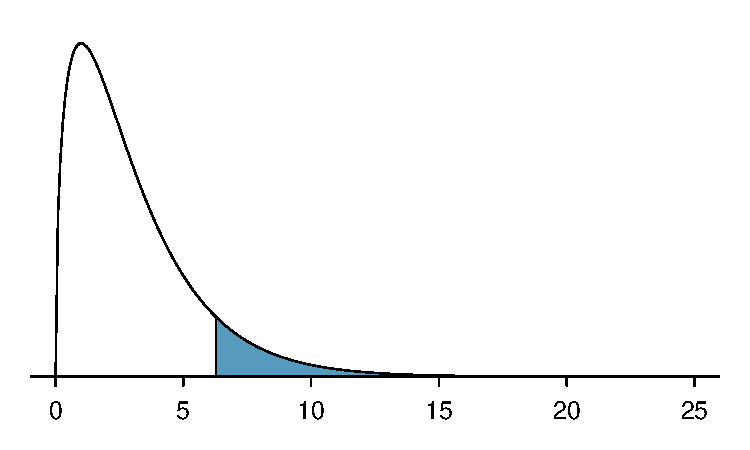
\includegraphics[width=0.475\textwidth]{ch_inference_for_props/figures/arrayOfFigureAreasForChiSquareDistribution/chiSquareAreaAbove6Point25WithDF3/chiSquareAreaAbove6Point25WithDF3}
\label{chiSquareAreaAbove6Point25WithDF3}
}
\subfigure[]{
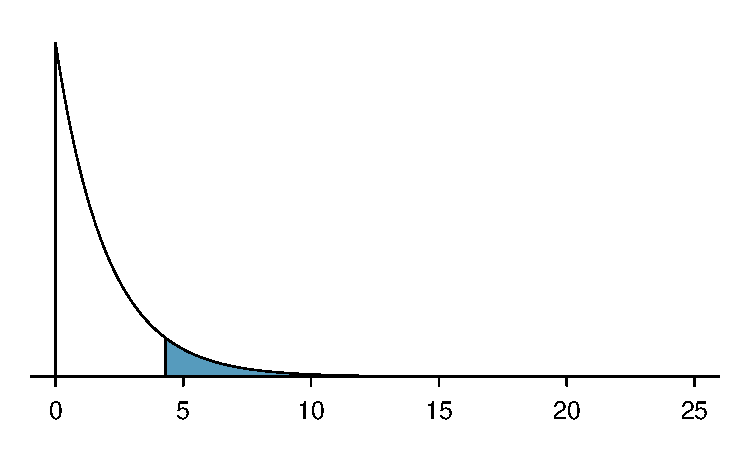
\includegraphics[width=0.475\textwidth]{ch_inference_for_props/figures/arrayOfFigureAreasForChiSquareDistribution/chiSquareAreaAbove4Point3WithDF2/chiSquareAreaAbove4Point3WithDF2}
\label{chiSquareAreaAbove4Point3WithDF2}
}
\subfigure[]{
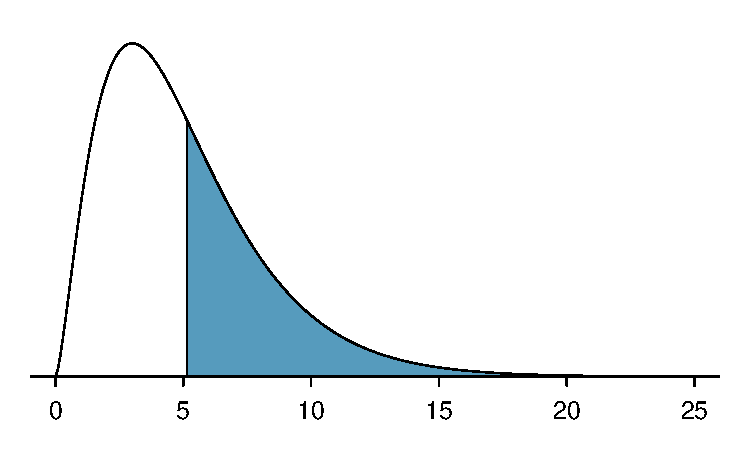
\includegraphics[width=0.475\textwidth]{ch_inference_for_props/figures/arrayOfFigureAreasForChiSquareDistribution/chiSquareAreaAbove5Point1WithDF5/chiSquareAreaAbove5Point1WithDF5}
\label{chiSquareAreaAbove5Point1WithDF5}
}
\subfigure[]{
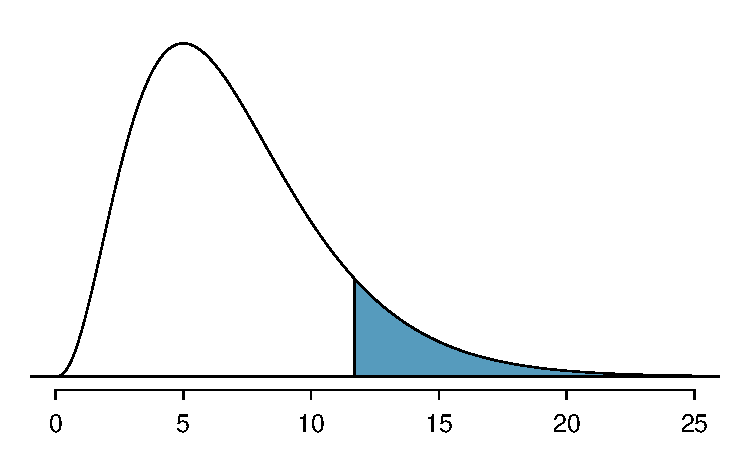
\includegraphics[width=0.475\textwidth]{ch_inference_for_props/figures/arrayOfFigureAreasForChiSquareDistribution/chiSquareAreaAbove11Point7WithDF7/chiSquareAreaAbove11Point7WithDF7}
\label{chiSquareAreaAbove11Point7WithDF7}
}
\subfigure[]{
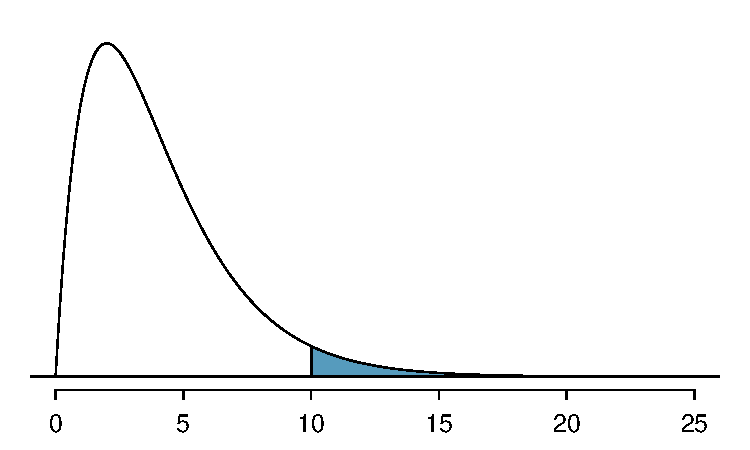
\includegraphics[width=0.475\textwidth]{ch_inference_for_props/figures/arrayOfFigureAreasForChiSquareDistribution/chiSquareAreaAbove10WithDF4/chiSquareAreaAbove10WithDF4}
\label{chiSquareAreaAbove10WithDF4}
}
\subfigure[]{
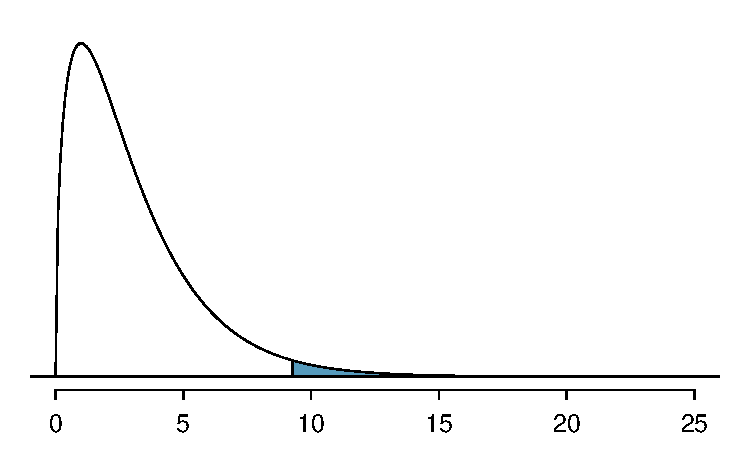
\includegraphics[width=0.475\textwidth]{ch_inference_for_props/figures/arrayOfFigureAreasForChiSquareDistribution/chiSquareAreaAbove9Point21WithDF3/chiSquareAreaAbove9Point21WithDF3}
\label{chiSquareAreaAbove9Point21WithDF3}
}
\caption{
\textbf{\subref{chiSquareAreaAbove6Point25WithDF3}}~Chi-square distribution with 3~degrees of freedom, area above 6.25 shaded.
\textbf{\subref{chiSquareAreaAbove4Point3WithDF2}}~2~degrees of freedom, area above 4.3 shaded.
\textbf{\subref{chiSquareAreaAbove5Point1WithDF5}}~5~degrees of freedom, area above 5.1 shaded.
\textbf{\subref{chiSquareAreaAbove11Point7WithDF7}}~7~degrees of freedom, area above 11.7 shaded.
\textbf{\subref{chiSquareAreaAbove10WithDF4}}~4~degrees of freedom, area above 10 shaded.
\textbf{\subref{chiSquareAreaAbove9Point21WithDF3}}~3~degrees of freedom, area above 9.21 shaded.
}
\label{arrayOfFigureAreasForChiSquareDistribution}
\end{figure}

\begin{examplewrap}
\begin{nexample}{We rarely observe the \emph{exact} value in the table. For instance, Figure~\ref{chiSquareAreaAbove4Point3WithDF2} shows the upper tail of a chi-square distribution with 2 degrees of freedom. The lower bound for this upper tail is at 4.3, which does not fall in Figure~\ref{chiSquareProbabilityTableShort}. Find the approximate tail area.}
The cutoff 4.3 falls between the second and third columns in the 2 degrees of freedom row. Because these columns correspond to tail areas of 0.2 and 0.1, we can be certain that the area shaded in Figure~\ref{chiSquareAreaAbove4Point3WithDF2} is between 0.1 and 0.2.
\end{nexample}
\end{examplewrap}



Using a calculator or statistical software allows us to get more precise areas under the chi-square curve than we can get from the table alone.

\begin{onebox}{\videohref{ti84_chisq_tail_area} TI-84: Finding an upper tail area under the chi-square curve}
\label{chisqtail}
Use the $\calctextmath{\chi^2}$\calctext{cdf} command to find areas under the chi-square curve.
\begin{enumerate}
\setlength{\itemsep}{0mm}
\item Hit \calcbutton{2ND} \calcbutton{VARS} (i.e. \calctext{DISTR}).
\item Choose \calctext{8:}$\calctextmath{\chi^2}$\calctext{cdf}.
\item Enter the lower bound, which is generally the chi-square value.
\item Enter the upper bound. Use a large number, such as 1000.
\item Enter the degrees of freedom.
\item Choose \calctext{Paste} and hit \calcbutton{ENTER}.
\end{enumerate}
TI-83: Do steps~1-2, then type the lower bound, upper bound, and degrees of freedom separated by commas. e.g. $\calctextmath{\chi^2}$\calctext{cdf(5, 1000, 3)}, and hit \calcbutton{ENTER}.\end{onebox}

\begin{onebox}{\videohref{casio_chisq_tail_area} Casio fx-9750GII: Finding an upper tail area under the chi-sq.~curve}
\begin{enumerate}
\setlength{\itemsep}{0mm}
\item Navigate to \calctext{STAT} (\calcbutton{MENU} button, then hit the \calcbutton{2} button or select \calctext{STAT}).
\item Choose the \calctext{DIST} option (\calcbutton{F5} button).
\item Choose the \calctext{CHI} option (\calcbutton{F3} button).
\item Choose the \calctext{Ccd} option (\calcbutton{F2} button).
\item If necessary, select the \calctext{Var} option (\calcbutton{F2} button).
\item Enter the \calctext{Lower} bound (generally the chi-square value).
\item Enter the \calctext{Upper} bound (use a large number, such as 1000).
\item Enter the degrees of freedom, \calctext{df}.
\item Hit the \calcbutton{EXE} button.
\end{enumerate}
\end{onebox}

\begin{exercisewrap}
\begin{nexercise}
Figure~\ref{chiSquareAreaAbove5Point1WithDF5} shows an upper tail for a chi-square distribution with 5 degrees of freedom and a cutoff of 5.1. Find the tail area using a calculator.\footnotemark\end{nexercise}
\end{exercisewrap}
\footnotetext{Use a lower bound of $5.1$, an upper bound of 1000, and $df = 5$.  The upper tail area is 0.4038.}

\begin{exercisewrap}
\begin{nexercise}
Figure~\ref{chiSquareAreaAbove11Point7WithDF7} shows a cutoff of 11.7 on a chi-square distribution with 7 degrees of freedom. Find the area of the upper tail.\footnotemark
\end{nexercise}
\end{exercisewrap}
\footnotetext{The area is 0.1109.}


\begin{exercisewrap}
\begin{nexercise}
Figure~\ref{chiSquareAreaAbove10WithDF4} shows a cutoff of 10 on a chi-square distribution with 4 degrees of freedom. Find the area of the upper tail.\footnotemark
\end{nexercise}
\end{exercisewrap}
\footnotetext{The area is 0.0404.}

\begin{exercisewrap}
\begin{nexercise}
Figure~\ref{chiSquareAreaAbove9Point21WithDF3} shows a cutoff of 9.21 with a chi-square distribution with 3 df. Find the area of the upper tail.\footnotemark
\end{nexercise}
\end{exercisewrap}
\footnotetext{The area is 0.0266.}


\D{\newpage}

%%
\subsection{Finding a p-value for a chi-square distribution}
\label{pValueForAChiSquareTest}

\index{data!racial make-up of jury|(}
In Section~\ref{chiSquareTestStatistic}, we identified a new test statistic ($\chi^2$) within the context of assessing whether there was evidence of racial/ethnic bias in how jurors were sampled. The null hypothesis represented the claim that jurors were randomly sampled and there was no racial/ethnic bias. The alternative hypothesis was that there was racial/ethnic bias in how the jurors were sampled.

We determined that a large $\chi^2$ value would suggest strong evidence favoring the alternative hypothesis: that there was racial/ethnic bias. However, we could not quantify what the chance was of observing such a large test statistic ($\chi^2=5.89$) if the null hypothesis actually was true. This is where the chi-square distribution becomes useful. If the null hypothesis was true and there was no racial/ethnic bias, then $\chi^2$ would follow a chi-square distribution, with three degrees of freedom in this case. Under certain conditions, the statistic $\chi^2$ follows a chi-square distribution with $k-1$ degrees of freedom, where $k$ is the number of bins or categories of the variable.

\begin{examplewrap}
\begin{nexample}{How many categories were there in the juror example? How many degrees of freedom should be associated with the chi-square distribution used for $\chi^2$?}
In the jurors example, there were $k=4$ categories: White, Black, Hispanic, and other. According to the rule above, the test statistic $\chi^2$ should then follow a chi-square distribution with $k-1 = 3$ degrees of freedom if $H_0$ is true.
\end{nexample}
\end{examplewrap}

Just like we checked sample~size conditions to use the normal model in earlier sections, we must also check a sample~size condition to safely model $\chi^2$ with a chi-square distribution. Each expected count must be at least 5. In the juror example, the expected counts were 198, 19.25, 33, and 24.75, all easily above~5, so we can model the $\chi^2$ test statistic, using a chi-square distribution.

\begin{examplewrap}
\begin{nexample}{If the null hypothesis is true, the test statistic $\chi^2=5.89$ would be closely associated with a chi-square distribution with three degrees of freedom. Using this distribution and test statistic, identify the p-value and state whether or not there is evidence of racial/ethnic bias in the juror selection.}
The chi-square distribution and p-value are shown in Figure~\ref{jurorHTPValueShown}. Because larger chi-square values correspond to stronger evidence against the null hypothesis, we shade the upper tail to represent the p-value. Using a calculator, we look at the chi-square curve with 3 degrees of freedom and find the area to the right of $\chi^2=5.89$.  This area, which corresponds to the p-value, is equal to 0.117.  This p-value is larger than the default significance level of 0.05, so we do not reject the null hypothesis.  In other words, the data do not provide convincing evidence of racial/ethnic bias in the juror selection.
\index{data!racial make-up of jury|)}
\end{nexample}
\end{examplewrap}

\begin{figure}[h]
\centering
\Figure{0.61}{jurorHTPValueShown}
\caption{The p-value for the juror hypothesis test is shaded in the chi-square distribution with $df=3$.}
\label{jurorHTPValueShown}
\end{figure}

The test that we just carried out regarding jury selection is known as the \termni{$\pmb{\chi^2}$ goodness of fit test}. It is called ``goodness of fit" because we test whether or not the proposed or expected distribution is a good fit for the observed data.

\begin{onebox}{Chi-square goodness of fit test for one-way table}
Suppose we are to evaluate whether there is convincing evidence that a set of observed counts $O_1$, $O_2$, ..., $O_k$ in $k$ categories are unusually different from what might be expected under a null hypothesis. Calculate the \emph{expected counts} that are based on the null hypothesis $E_1$, $E_2$, ..., $E_k$. If each expected count is at least 5 and the null hypothesis is true, then the test statistic below follows a chi-square distribution with $k-1$ degrees of freedom:
\begin{align*}
\chi^2 = \frac{(O_1 - E_1)^2}{E_1} + \frac{(O_2 - E_2)^2}{E_2} + \cdots + \frac{(O_k - E_k)^2}{E_k}
\end{align*}
The p-value for this test statistic is found by looking at the upper tail of this chi-square distribution. We consider the upper tail because larger values of $\chi^2$ would provide greater evidence against the null hypothesis.\end{onebox}

\begin{onebox}{Conditions for the chi-square goodness of fit test}
The chi-square goodness of fit test requires the test statistic to be well modeled by a chi-square distribution.  This will be valid when the observations are independent and the expected counts are large.  If these conditions are not met, the chi-square goodness of fit test should not be used.\vspace{-1mm}
\begin{description}
\setlength{\itemsep}{0mm}
\item[Independence.] The observations can be considered independent if the data come from a random process.  If randomly sampling without replacement from a finite population, the observations can be considered independent when sampling less than 10\% of the population.  
\item[Large expected counts.] In order for the $\chi^2$-statistic to follow the chi-square distribution, each particular bin or category must have at least \mbox{5~expected} cases under the assumption that the null hypothesis is true.
\vspace{-2mm}
\end{description}
\end{onebox}


\D{\newpage}

%%
\subsection{Evaluating goodness of fit for a distribution}

\begin{onebox}{Goodness of fit test for a one-way table}
 When there is one sample and we are comparing the distribution of a categorical variable to a specified or population distribution, e.g. using sample values to determine if a machine is producing M\&M's with the specified distribution of color, 
\\
\\
\inferencestep{Identify} Identify the hypotheses and the significance level, $\alpha$. \vspace{-1mm}
\begin{itemize}
\setlength{\itemsep}{0mm}
\item[]  $H_0$: The distribution of [...] matches the specified or population distribution. 
\item[] $H_A$: The distribution of [...] doesn't match the specified or population distribution.
\end{itemize}
\inferencestep{Choose} Choose the correct test procedure and identify it by name.\vspace{-1mm}
\begin{itemize}
\item[]  Here we use a \termni{\pmb{$\chi^2$} goodness of fit test}.
\end{itemize}
\inferencestep{Check} Check that the test statistic follows a chi-square distribution.\vspace{-1mm}
\begin{itemize}
\setlength{\itemsep}{0mm}
\item[] 1.  Independence:  Data come from a random sample or random process.  If sampling 
\item[] \quad \  without replacement, check that the sample size is less than 10\% of the population
\item[] \quad \ size.
\item[] 2.   Expected counts:  All expected counts are $\ge$ 5. 
\end{itemize}
\inferencestep{Calculate} Calculate the $\chi^2$-statistic, $df$, and p-value.\vspace{-1mm}  
\begin{itemize}
\setlength{\itemsep}{0mm}
\item[] test statistic:  $\chi^2 =\sum{ \frac{\text{(observed } - \text{ expected})^2}{\text{expected}}}$ 
\item[] $df =$ \# of categories $-$ 1
\item[] p-value = (area to the \emph{right} of $\chi^2$-statistic with the appropriate $df$)
\end{itemize}
\inferencestep{Conclude} Compare the p-value to $\alpha$, and draw a conclusion in context.
\begin{itemize}\vspace{-1mm}
\setlength{\itemsep}{0mm}
\item[] If the p-value is $< \alpha$, reject $H_0$; there is sufficient evidence that [$H_A$ in context]. 
\item[] If the p-value is $> \alpha$, do not reject $H_0$; there is not sufficient evidence that [$H_A$ in context].
\end{itemize}
\end{onebox}


Have you ever wondered about the color distribution of M\&M's$^{\text{\textregistered}}$?  If so, then you will be glad to know that Rick Wicklin, a statistician working at the statistical software company SAS, wondered about this too.  But he did more than wonder; he decided to collect data to test whether the distribution of M\&M colors was consistent with the stated distribution published on the Mars website in 2008.  Starting at end of 2016, over the course of several weeks, he collected a sample of 712 candies, or about 1.5 pounds.  We will investigate his results in the next example.  You can read about his adventure in the Quartz article cited in the footnote below.\footnotemark 
\footnotetext{\oiRedirect{textbook-mandms}{https://qz.com/918008/the-color-distribution-of-mms-as-determined-by-a-phd-in-statistics}. }

\D{\newpage}

\begin{examplewrap}
\begin{nexample}
{The stated color distribution of M\&M's on the Mars website in 2008 is shown in the table below, along with the observed percentages from Rick Wicklin's sample of size 712. (See the paragraph before this example for more background.) \\
\begin{center}
\begin{small}
\begin{tabular}{ll ccc ccc}
\hline
	 & \hspace{1mm} & Blue & Orange & Green & Yellow & Red & Brown\\
\hline
website percentages (2008):&		& 24\% & 20\% & 16\% & 14\% & 13\% & 13\%  \\
observed percentages:&		& 18.7\% & 18.7\% & 19.5\% & 14.5\% & 15.1\% & 13.5\%  \\
\hline
\end{tabular}
\end{small}
\end{center}


Is there evidence at the 5\% significance level that the distribution of M\&M's in 2016 were different from the stated distribution on the website in 2008? Use the five step framework to organize your work. }

\begin{description}
\item[\inferencestep{Identify}]  
We will test the following hypotheses at the $\alpha=0.05$ significance level.\\
\\
$H_0$:  The distribution of M\&M colors is the same as the stated distribution in 2008. \\
$H_A$: The distribution of M\&M colors is different than the stated distribution in 2008.
 

\item[\inferencestep{Choose}] Because we have one variable (color), broken up into multiple categories, we choose the \mbox{chi-square goodness of fit test.}
\item[\inferencestep{Check}]  We must verify that the test statistic follows a chi-square distribution.  Note that there is only one sample here.  The website percentages are considered fixed -- they are not the result of a sample and do not have sampling variability associated with them.  To carry out the chi-square goodness of fit test, we will have to assume that Wicklin's sample can be considered a random sample of M\&M's.  We note that the total population size of M\&M's is much larger than 10 times the sample size of 712.  Next, we need to find the expected counts.  Here, $n=712$.  If $H_0$ is true, then we would expect 24\% of the M\&M's to be Blue, 20\% to be Orange, etc.  So the expected counts can be found as:

\begin{small}
\begin{tabular}{ll ccc ccc}
\hline
	 & \hspace{1mm} & Blue & Orange & Green & Yellow & Red & Brown\\
\hline
expected counts:&		& 0.24(712) &  0.20(712) & 0.16(712) & 0.14(712) & 0.13(712) & 0.13(712)  \\
&		& = 170.9 &  = 142.4 & = 113.9 & = 99.6 & = 92.6 & = 92.6\\ 
\hline
\end{tabular}
\end{small}

\item[ \inferencestep{Calculate} ]  We will calculate the chi-square statistic, degrees of freedom, and the p-value.\\
To calculate the chi-square statistic, we need the observed counts as well as the expected counts.  To find the observed counts, we use the observed percentages.  For example, 18.7\% of $712 = 0.187(712)=133$.

\begin{center}
\begin{small}
\begin{tabular}{ll ccc ccc}
\hline
	 & \hspace{1mm} & Blue & Orange & Green & Yellow & Red & Brown\\
\hline
observed counts:&		& 133 & 133 & 139 & 103 & 108 & 96  \\
expected counts:&		& 170.9 &  142.4 & 113.9 & 99.6 & 92.6 & 92.6\\
\hline
\end{tabular}
\end{small}
\end{center}
\begin{small}
\begin{align*}
\chi^2
  =& \sum{\frac{\text{(observed } - \text{ expected})^2}
      {\text{expected}}}\\
  =& \frac{(133 - 170.9)^2}{170.9}
      + \frac{(133 - 142.4)^2}{142.4}
      %+ \frac{(139 - 113.9)^2}{113.9}
      %+ \frac{(103 - 99.6)^2}{99.6}
      + \cdots
      + \frac{(108 - 92.6)^2}{92.6}
      + \frac{(96 - 92.6)^2}{92.6}\\
=&8.41+0.62+5.53+0.12+2.56+0.12\\
=&17.36
\end{align*}
\end{small}

Because there are six colors, the degrees of freedom is $6-1=5$.
\\In a chi-square test, the p-value is always the area to the \emph{right} of the chi-square statistic.  Here, the area to the right of 17.36 under the chi-square curve with 5 degrees of freedom is $0.004$.  
\item[\inferencestep{Conclude}]  The p-value of 0.004 is $< 0.05$, so we reject $H_0$; there is sufficient evidence that the distribution of M\&M's does not match the stated distribution on the website in 2008.  
\end{description}
\end{nexample}
\end{examplewrap}

\begin{examplewrap}
\begin{nexample}
{For Wicklin's sample, which color showed the most prominent difference from the stated website distribution in 2008?}
We can compare the website percentages with the observed percentages.  However, another approach is to look at the terms used when calculating the chi-square statistic.  We note that the largest term, 8.41, corresponds to Blue.  This means that the observed number for Blue was, relatively speaking, the farthest from the expected number among all of the colors.  This is consistent with the observation that the largest difference in website percentage and observed percentage is for Blue (24\% vs 18.7\%).  Wicklin observed far fewer Blue M\&M's than would have been expected if the website percentages were still true.
\end{nexample}
\end{examplewrap}


\D{\newpage}

%%
\subsection{Calculator: chi-square goodness of fit test}
\label{GOF}

\begin{onebox}{\videohref{ti84_chisq_GOF_test} TI-84: Chi-square goodness of fit test\vspace{0.5mm}}
Use \calctext{STAT}, \calctext{TESTS}, $\calctextmath{\chi^2}$\calctext{GOF-Test}.
\begin{enumerate}
\setlength{\itemsep}{0mm}
\item Enter the observed counts into list \calctext{L1} and the expected counts into list \calctext{L2}.
\item Choose \calctext{STAT}.
\item Right arrow to \calctext{TESTS}.
\item Down arrow and choose \calctext{D:}$\calctextmath{\chi^2}$\calctext{GOF-Test}.
\item Leave \calctext{Observed:~L1} and \calctext{Expected:~L2}.
\item Enter the degrees of freedom after \calctext{df}:
\item Choose \calctext{Calculate} and hit \calcbutton{ENTER}, which returns: \\[1mm]
\begin{tabular}{l ll}
$\calctextmath{\chi^2}$ & chi-square test statistic \\
\calctext{p} & p-value \\
\calctext{df} & degrees of freedom
\end{tabular}
\end{enumerate}
TI-83: Unfortunately the TI-83 does not have this test built in. To carry out the test manually, make list \calctext{L3 = (L1 - L2)}$\calctextmath{^2}$\calctext{ / L2} and do \calctext{1-Var-Stats} on \calctext{L3}. The sum of \calctext{L3} will correspond to the value of $\chi^2$ for this test.\end{onebox}

\begin{onebox}{\videohref{casio_chisq_GOF_test} Casio fx-9750GII: Chi-square goodness of fit test\vspace{0.5mm}}
\begin{enumerate}
\setlength{\itemsep}{0mm}
\item Navigate to \calctext{STAT} (\calcbutton{MENU} button, then hit the \calcbutton{2} button or select \calctext{STAT}).
\item Enter the observed counts into a list (e.g. \calctext{List 1}) and the expected counts into list (e.g. \calctext{List 2}).
\item Choose the \calctext{TEST} option (\calcbutton{F3} button).
\item Choose the \calctext{CHI} option (\calcbutton{F3} button).
\item Choose the \calctext{GOF} option (\calcbutton{F1} button).
\item Adjust the \calctext{Observed} and \calctext{Expected} lists to the corresponding list numbers from Step~2.
\item Enter the degrees of freedom, \calctext{df}.
\item Specify a list where the contributions to the test statistic will be reported using~\calctext{CNTRB}. This list number should be different from the others.
\item Hit the \calcbutton{EXE} button, which returns \\[1mm]
  \begin{tabular}{l ll}
  $\calctextmath{\chi^2}$ & chi-square test statistic \\
  \calctext{p} & p-value \\
  \calctext{df} & degrees of freedom \\
  \calctext{CNTRB} & list showing the test statistic contributions
  \end{tabular}
\end{enumerate}
\end{onebox}


\begin{exercisewrap}
\begin{nexercise}
Use the table below and a calculator to find the $\chi^2$-statistic and p-value for chi-square goodness of fit test.\footnotemark
\begin{center}
\begin{tabular}{ll ccc ccc}
\hline
	 & \hspace{1mm} & Blue & Orange & Green & Yellow & Red & Brown\\
\hline
observed counts:&		& 133 & 133 & 139 & 103 & 108 & 96  \\
expected counts:&		& 170.9 &  142.4 & 113.9 & 99.6 & 92.6 & 92.6\\
\hline
\end{tabular}
\end{center}

\end{nexercise}
\end{exercisewrap}
\footnotetext{Enter the observed counts into \calctext{L1} and the expected counts into  \calctext{L2}.    the \calctext{GOF} test.  Make sure that \calctext{Observed:} is \calctext{L1} and \calctext{Expected:} is \calctext{L2}.  Let \calctext{df:} be 5.  You should find that $\chi^2=17.36$ and $\text{p-value}=0.004$.}

\index{chi-square goodness of fit test@$\chi^2$ goodness of fit test|)}
\D{\newpage}

%%
\subsection*{Section summary} 
\noindent The inferential procedures we saw in the first two sections of this chapter are based on the test statistic following a \textit{normal distribution}.  In this section, we introduced a new distribution called the chi-square distribution.  

\begin{itemize}

\item While a normal distribution is defined by its mean and standard deviation, the chi-square distribution is defined by just one parameter called \termsub{degrees of freedom}{degrees of freedom (df)!chi-square}.  
\item For a chi-square distribution, as the degrees of freedom increases:  the center increases, the spread increases, and the shape becomes more symmetric and more normal.\footnote{Technically, however, it is always right skewed.}


\item When we want to see if a model is a good fit for observed data or if data is representative of a particular population, we can use a \termni{$\pmb{\chi^2}$ goodness of fit test}\index{chi-square goodness of fit test@$\chi^2$ goodness of fit test}.  This test is used when there is one variable with multiple categories (bins) that can be arranged in a \textbf{one-way table}.

\item In a chi-square goodness of fit test, we calculate a \termsub{$\pmb{\chi^2}$-statistic}{chi-square statistic@$\chi^2$-statistic}, which is a measure of how far the observed counts in the sample are from the expected counts, relative to the expected counts, under the null hypothesis. $\chi^2 =\sum{ \frac{\text{(observed } - \text{ expected})^2}{\text{expected}}}$.
\begin{itemize}\vspace{-1mm}
\item Always use whole numbers (counts) for the observed values, not proportions or percents.
\item For each category, the expected counts can be found by multiplying the sample~size by the expected proportion under the null hypothesis.  Expected counts do \emph{not} need to be integers.  
\end{itemize}

\item A larger $\chi^2$ represents greater deviation between the observed values and the expected values, relative to the expected values.  For a fixed degrees of freedom, a larger $\chi^2$ value leads to a smaller p-value, providing greater evidence against $H_0$. 


\item \textbf{\pmb{$\chi^2$}  tests for a one-way table}.  When there is one sample and we are comparing the distribution of a categorical variable to a specified or population distribution, e.g. using sample values to determine if a machine is producing M\&M's with the specified distribution of color, the hypotheses can often be written as:
\begin{itemize}
\item[] $H_0$: The distribution of [...] matches the specified or population distribution. 
\item[] $H_A$: The distribution of [...] doesn't match the specified or population distribution. 
\end{itemize}

\item[] We test these hypotheses at the $\alpha$ significance level using a \termni{\pmb{$\chi^2$} goodness of fit test}\index{chi-square goodness of fit test@$\chi^2$ goodness of fit test}.\\
\item For the $\chi^2$ goodness of fit test, we check the following conditions to verify that the test statistic follows a chi-square distribution.  
\begin{itemize}
\item[] 1.  Independence:  Data come from a random sample or random process.  When sampling 
\item[] \quad \ without replacement, check that sample size is less than 10\% of the population size.
\item[] 2.  Expected counts:  All expected counts are $\ge$ 5.
\end{itemize}

\item We calculate the test statistic as follows:
\begin{itemize}
\item[] test statistic:  $\chi^2 =\sum{ \frac{\text{(observed } - \text{ expected})^2}{\text{expected}}}$; \quad \quad $df =$ \# of categories $-$ 1
\end{itemize}
\item The p-value is the area to the \emph{right} of the $\chi^2$-statistic under the chi-square curve with the appropriate $df$.

\item For a $\chi^2$ test, the p-value corresponds to the probability of getting a test statistic as large as we got or larger, assuming the null hypothesis is true and assuming the chi-square model holds.
\end{itemize}


%%%%%%%%Section Exercises
{\exercisesheader{}

% 27 - tf_chisq_1

\eoce{\qt{True or false, Part I\label{tf_chisq_1}} Determine if the statements below 
are true or false. For each false statement, suggest an alternative wording to 
make it a true statement.
\begin{parts}
\item The chi-square distribution, just like the normal distribution, has two 
parameters, mean and standard deviation.
\item The chi-square distribution is always right skewed, regardless of the 
value of the degrees of freedom parameter.
\item The chi-square statistic is always greater than or equal to 0.
\item As the degrees of freedom increases, the shape of the chi-square 
distribution becomes more skewed.
\end{parts}
}{}

% 28 - tf_chisq_2

\eoce{\qt{True or false, Part II\label{tf_chisq_2}} Determine if the statements below 
are true or false. For each false statement, suggest an alternative wording to 
make it a true statement.
\begin{parts}
\item As the degrees of freedom increases, the mean of the chi-square 
distribution increases.
\item If you found $\chi^2 = 10$ with $df = 5$ you would fail to reject $H_0$ 
at the 5\% significance level.
\item When finding the p-value of a chi-square test, we always shade the tail 
areas in both tails.
\item As the degrees of freedom increases, the variability of the chi-square 
distribution decreases.
\end{parts}
}{}

% 29 - opensource_text_chisq_GOF

\eoce{\qt{Open source textbook\label{opensource_text_chisq_GOF}} \videosolution{ahss_eoce_sol-opensource_text_chisq_GOF} A professor using 
an open source introductory statistics book predicts that 60\% of the 
students will purchase a hard copy of the book, 25\% will print it out from 
the web, and 15\% will read it online. At the end of the semester he asks his 
students to complete a survey where they indicate what format of the book 
they used. Of the 126 students, 71 said they bought a hard copy of the book, 
30 said they printed it out from the web, and 25 said they read it online.
\begin{parts}
\item State the hypotheses for testing if the professor's predictions were 
inaccurate.
\item How many students did the professor expect to buy the book, print the 
book, and read the book exclusively online?
\item List the conditions required for the chi-square goodness of fit test and discuss whether they are satisfied.
\item Assume conditions are sufficiently met.  Calculate the chi-squared statistic, the degrees of freedom associated 
with it, and the p-value.
\item Based on the p-value calculated in part (d), what is the conclusion of 
the hypothesis test? Interpret your conclusion in this context.
\end{parts}
}{}

% 30 - barking_deer_chisq_GOF

\eoce{\qt{Barking deer\label{barking_deer_chisq_GOF}}
Microhabitat factors associated with forage and bed sites
of barking deer in Hainan Island, China were examined.
In this region woods make up 4.8\% of the land,
cultivated grass plot makes up 14.7\%, and deciduous forests
make up 39.6\%.
Of the 426 sites where the deer forage, 4 were categorized
as woods, 16 as cultivated grassplot, and 61 as deciduous forests.
The table below summarizes these data.\footfullcite{Teng:2004}
\begin{center}
\begin{tabular}{c c c c c}
Woods	& Cultivated grassplot	& Deciduous forests	 & Other & Total \\
\hline 
4		& 16					& 61			     & 345	 & 426 \\
\end{tabular}
\end{center}

\noindent \begin{minipage}[c]{0.7\textwidth}
\begin{parts}
\item Write the hypotheses for testing if barking deer prefer to forage in 
certain habitats over others.
\item What type of test can we use to answer this research question?
\item Check if the assumptions and conditions required for this test are 
satisfied.
\item Assume the conditions for the test are met.  Do these data provide convincing evidence that barking deer prefer to 
forage in certain habitats over others? Conduct an appropriate hypothesis 
test to answer this research question, and acknowledge any assumptions you had to make to carry out this test.
\end{parts}
\end{minipage}
\begin{minipage}[c]{0.03\textwidth}
$\:$ \\
\end{minipage}
\begin{minipage}[c]{0.28\textwidth}
\begin{center}

\includegraphics[width=0.7\textwidth]{ch_inference_for_props/figures/eoce/barking_deer_chisq_GOF/barking_deer.jpg} \\
{\footnotesize Photo by Shrikant Rao (\oiRedirect{textbook-flickr_shrikant_rao_barking_deer}{http://flic.kr/p/4Xjdkk}) \oiRedirect{textbook-CC_BY_2}{CC~BY~2.0~license}}
\end{center}
\end{minipage}
}{}
}


%_________________________________________________
\section[Homogeneity and independence in two-way tables]{Chi-square tests in two-way tables }
\label{twoWayTablesAndChiSquare}

\sectionintro{
\noindent%
We encounter two-way tables in this section, and we learn about two new and closely related chi-square tests.
We will answer questions such as the following:
\begin{itemize}
\item Does the phrasing of the question affect how likely sellers are to disclose problems with a product?
\item Is gender associated with whether Facebook users know how to adjust their privacy settings?
\item Is political affiliation associated with support for the use of full body scans at airports?
\end{itemize}


%%
\subsection*{Learning objectives}

\begin{enumerate}
\setlength{\itemsep}{0mm}
\item Calculate the expected counts and degrees of freedom for a chi-square test involving a two-way table.

\item State and verify whether or not the conditions for a chi-square test for a two-way table are met.

\item Explain the difference between the chi-square test for homogeneity and chi-square test for independence.

\item Carry out a complete hypothesis test for homogeneity and for independence.

\end{enumerate}
}


\D{\newpage}

%%
\subsection{Introduction}
Google is constantly running experiments to test new search algorithms. For example, Google might test three algorithms using a sample of 10,000 google.com search queries. Figure~\ref{googleSearchAlgorithmByAlgorithmOnly} shows an example of 10,000 queries split into three algorithm groups.\footnote{Google regularly runs experiments in this manner to help improve their search engine. It is entirely possible that if you perform a search and so does your friend, that you will have different search results. While the data presented in this section resemble what might be encountered in a real experiment, these data are simulated.} The group sizes were specified before the start of the experiment to be 5000 for the current algorithm and 2500 for each test algorithm.

\begin{figure}[h]
\centering
\begin{tabular}{ll ccc ll}
\hline
Search algorithm	 & \hspace{1mm} & current & test 1 & test 2 & \hspace{1mm} & Total \\
Counts &		& 5000 & 2500 & 2500 & & 10000 \\
\hline
\end{tabular}
\caption{Experiment breakdown of test subjects into three search groups.}
\label{googleSearchAlgorithmByAlgorithmOnly}
\end{figure}


\begin{examplewrap}
\begin{nexample}{What is the ultimate goal of the Google experiment? What are the null and alternative hypotheses, in regular words?}
The ultimate goal is to see whether there is a difference in the performance of the algorithms. The hypotheses can be described as the following:\D{\vspace{-2mm}}
\begin{itemize}
\setlength{\itemsep}{0mm}
\item[$H_0$:] The algorithms each perform equally well.
\item[$H_A$:] The algorithms do not perform equally well.
\end{itemize}
\end{nexample}
\end{examplewrap}

In this experiment, the explanatory variable is the search algorithm. However, an outcome variable is also needed. This outcome variable should somehow reflect whether the search results align with the user's interests. One possible way to quantify this is to determine whether (1)~there was no new, related search, and the user clicked one of the links provided, or (2)~there was a new, related search performed by the user. Under scenario~(1), we might think that the user was satisfied with the search results. Under scenario~(2), the search results probably were not relevant, so the user tried a second search.

Figure~\ref{googleSearchAlgorithmByAlgorithmAndPerformanceWithTotals} provides the results from the experiment. These data are very similar to the count data in Section~\ref{oneWayChiSquare}. However, now the different combinations of two variables are binned in a \emph{two-way} table. In examining these data, we want to evaluate whether there is strong evidence that at least one algorithm is performing better than the others. To do so, we apply a chi-square test to this two-way table. The ideas of this test are similar to those ideas in the one-way table case. However, degrees of freedom and expected counts are computed a little differently than before.

\begin{figure}[h]
\centering
\quad \quad \quad \quad Search algorithm \\
\begin{tabular}{ll ccc ll}
\hline
 & \hspace{1mm} & current & test 1 & test 2 & \hspace{1mm} & Total \\
\hline
No new search				   & & 3511    & 1749 & 1818 & 				& 7078 \\
New search				   & & 1489    & 751	& 682    &				& 2922 \\
\hline
Total						   & & 5000    & 2500 & 2500 & 				& 10000 \\
\hline
\end{tabular}
\caption{Results of the Google search algorithm experiment.}
\label{googleSearchAlgorithmByAlgorithmAndPerformanceWithTotals}
\end{figure}

\begin{onebox}{What is so different about one-way tables and two-way tables?}
A one-way table describes counts for each outcome in a single variable. A two-way table describes counts for \emph{combinations} of outcomes for two variables. When we consider a two-way table, we often would like to know, are these variables related in any way?\end{onebox}

The hypothesis test for this Google experiment is really about assessing whether there is statistically significant evidence that the choice of the algorithm affects whether a user performs a second search. In other words, the goal is to check whether the three search algorithms perform differently.


\D{\newpage}

%%
\subsection{Expected counts in two-way tables}

\begin{examplewrap}
\begin{nexample}{From the experiment, we estimate the proportion of users who were satisfied with their initial search (no new search) as $7078/10000 = 0.7078$. If there really is no difference among the algorithms and 70.78\% of people are satisfied with the search results, how many of the 5000 people in the ``current algorithm'' group would be expected to not perform a new search?} \label{googleExampleComputingTheExpectedNumberOfCurrentGroupWithNoNewSearch}
About 70.78\% of the 5000 would be satisfied with the initial search:
$$ 0.7078\times 5000 = 3539\text{ users} $$
That is, if there was no difference between the three groups, then we would expect 3539 of the current algorithm users not to perform a new search.
\end{nexample}
\end{examplewrap}

\begin{exercisewrap}
\begin{nexercise}\label{googleExampleComputingTheExpectedNumberOfNewAlgGroupWithNoNewSearch}
Using the same rationale described in Example~\ref{googleExampleComputingTheExpectedNumberOfCurrentGroupWithNoNewSearch}, about how many users in each test group would not perform a new search if the algorithms were equally helpful?\footnotemark
\end{nexercise}
\end{exercisewrap}
\footnotetext{We would expect $0.7078*2500 = 1769.5$. It is okay that this is a fraction.}

We can compute the expected number of users who would perform a new search for each group using the same strategy employed in Example~\ref{googleExampleComputingTheExpectedNumberOfCurrentGroupWithNoNewSearch} and Guided Practice~\ref{googleExampleComputingTheExpectedNumberOfNewAlgGroupWithNoNewSearch}. These expected counts were used to construct Figure~\ref{googleSearchAlgorithmByAlgorithmAndPerformanceWithExpectedCounts}, which is the same as Figure~\ref{googleSearchAlgorithmByAlgorithmAndPerformanceWithTotals}, except now the expected counts have been added in parentheses.

\begin{figure}[h]
\centering
\begin{tabular}{l lll lll lll l}
\hline
Search algorithm\hspace{2mm} & \multicolumn{2}{l}{current} &&
					\multicolumn{2}{l}{test 1} &&
					\multicolumn{2}{l}{test 2} & \hspace{0mm} & Total \\
\hline
No new search		   & 3511 &\highlightO{\footnotesize(3539)}    &&
					1749 &\highlightO{\footnotesize(1769.5)}	&&
					1818 &\highlightO{\footnotesize(1769.5)} &	& 7078 \\
New search		   & 1489 &\highlightO{\footnotesize(1461)}    &&
					751 &\highlightO{\footnotesize(730.5)}	&&
					682 &\highlightO{\footnotesize(730.5)}    &		& 2922 \\
\hline
Total				   & 5000 &&& 	2500 &&& 	2500 &&& 	10000 \\
\hline
\end{tabular}
\caption{The observed counts and the \highlightO{(expected counts)}.}
\label{googleSearchAlgorithmByAlgorithmAndPerformanceWithExpectedCounts}
\end{figure}

The examples and exercises above provided some help in computing expected counts. In general, expected counts for a two-way table may be computed using the row totals, column totals, and the table total. For instance, if there was no difference between the groups, then about 70.78\% of each column should be in the first row:
\begin{align*}
0.7078\times (\text{column 1 total}) &= 3539 \\
0.7078\times (\text{column 2 total}) &= 1769.5 \\
0.7078\times (\text{column 3 total}) &= 1769.5
\end{align*}
Looking back to how the fraction 0.7078 was computed -- as the fraction of users who did not perform a new search ($7078/10000$) -- these three expected counts could have been computed as
\begin{align*}
\left(\frac{\text{row 1 total}}{\text{table total}}\right)\text{(column 1 total)} &= 3539 \\
\left(\frac{\text{row 1 total}}{\text{table total}}\right)\text{(column 2 total)} &= 1769.5 \\
\left(\frac{\text{row 1 total}}{\text{table total}}\right)\text{(column 3 total)} &= 1769.5
\end{align*}
This leads us to a general formula for computing expected counts in a two-way table when we would like to test whether there is strong evidence of an association between the column variable and row variable.

\D{\newpage}

\begin{onebox}{Computing expected counts in a two-way table}
To identify the expected count for the $i^{th}$ row and $j^{th}$ column, compute
$$\text{Expected Count}_{\text{row }i,\text{ col }j} = \frac{(\text{row $i$ total}) \times  (\text{column $j$ total})}{\text{table total}}\vspace{2mm}$$\end{onebox}


%%
\subsection{The chi-square test for homogeneity in two-way tables}
\index{chi-square test for homogeneity@$\chi^2$ test for homogeneity|(}

The chi-square test statistic for a two-way table is found the same way it is found for a one-way table. For each table count, compute
\begin{align*}
&\text{General formula}& &\frac{(\text{observed count } - \text{ expected count})^2}{\text{expected count}} \\
&\text{Row 1, Col 1}& &\frac{(3511 - 3539)^2}{3539} = 0.222 \\
&\text{Row 1, Col 2}& &\frac{(1749 - 1769.5)^2}{1769.5} = 0.237 \\
& \hspace{9mm}\vdots & &\hspace{13mm}\vdots \\
&\text{Row 2, Col 3}& &\frac{(682 - 730.5)^2}{730.5} = 3.220
\end{align*}
Adding the computed value for each cell gives the chi-square test statistic $\chi^2$:
$$\chi^2 = 0.222 + 0.237 + \dots + 3.220 = 6.120$$
Just like before, this test statistic follows a chi-square distribution. However, the degrees of freedom is computed a little differently for a two-way table.\footnote{Recall: in the one-way table, the degrees of freedom was the number of groups minus 1.} For two way tables, the degrees of freedom is equal to
\begin{align*}
df = \text{(number of rows - 1)}\times \text{(number of columns - 1)}
\end{align*}
In our example, the degrees of freedom is
\begin{align*}
df = (2-1)\times (3-1) = 2
\end{align*}
If the null hypothesis is true (i.e. the algorithms are equally useful), then the test statistic $\chi^2 = 6.12$ closely follows a chi-square distribution with 2 degrees of freedom. Using this information, we can compute the p-value for the test, which is depicted in Figure~\ref{googleHTForDiffAlgPerformancePValue}.

\begin{onebox}{Computing degrees of freedom for a two-way table}
When using the chi-square test to a two-way table, we use
$$ df = (R-1)\times (C-1) $$
where $R$ is the number of rows in the table and $C$ is the number of columns.\end{onebox}

\begin{onebox}{Use two-proportion methods for 2-by-2 contingency tables}
When analyzing 2-by-2 contingency tables, use the two-proportion methods introduced in Section~\ref{differenceOfTwoProportions}.\end{onebox}

\begin{figure}[h]
\centering
\Figure{0.7}{googleHTForDiffAlgPerformancePValue}
\caption{Computing the p-value for the Google hypothesis test.}
\label{googleHTForDiffAlgPerformancePValue}
\end{figure}

\D{\newpage}

\begin{onebox}{Conditions for the chi-square test for homogeneity}
There are two conditions that must be checked before performing a chi-square test for homogeneity. If these conditions are not met, this test should not be used.\vspace{-1mm}
\begin{description}
\setlength{\itemsep}{0mm}
\item[Independence.] Data should be come from multiple independent random samples or from a randomized experiment with multiple treatments. Data can then be organized into a two-way table.  When sampling without replacement, the sample size should be less than 10\% of the population size for each sample.
\item[Large expected counts. ] All of the cells in the two-way table must  have at least 5~expected cases under the assumption that the null hypothesis is true.
\end{description}\end{onebox}

\begin{examplewrap}
\begin{nexample}{Compute the p-value and draw a conclusion about whether the search algorithms have different performances.}
Here, found that the degrees of freedom for this $3\times 2$ table is 2.  The p-value corresponds to the area under the chi-square curve with 2 degrees of freedom to the \emph{right} of $\chi^2=6.120$.  Using a calculator, we find that the p-value = 0.047.  Using an $\alpha=0.05$ significance level, we reject $H_0$.  That is, the data provide convincing evidence that there is some difference in performance among the algorithms.
\index{data!search algorithm|)}
\end{nexample}
\end{examplewrap}

Notice that the conclusion of the test is that there is some difference in performance among the algorithms.  This chi-square test does not tell us \emph{which} algorithm performed better than the others.  To answer this question, we could compare the relevant proportions or construct bar graphs.   The proportion that resulted in the new search can be calculated as 
\begin{align*}
\text{current:} \frac{1489}{5000} = 0.298 \quad \text{test 1:} \frac{751}{2500} = 0.300 \quad \text{test 2:} \frac{682}{2500} = 0.136.
\end{align*}
This suggests that the test 2 algorithm performed better than the current algorithm and test 1 algorithm, because it led to fewer new searches; however, to formally test this specific claim we would need to use a test that includes a multiple comparisons correction, which is beyond the scope of this textbook.



A careful reader may have noticed that when there are exactly 2 random samples or treatments and the counts can be arranged in a $2\times 2$ table, both a chi-square test for homogeneity \emph{and} a 2-proportion Z-test could apply.   In this case, the chi-square test for homogeneity and the two-sided 2-proportion Z-test are equivalent, meaning that they produce the same p-value.\footnote{Sometimes the success-failure condition for the Z-test is weakened to require the number of successes and failures to be at least 5, making it consistent with the chi-square condition that expected counts must at least 5.}


%	Approve	Disapprove
%Obama	56	41
%Dem	49	43
%Rep	36	56
%http://www.people-press.org/2012/03/14/romney-leads-gop-contest-trails-in-matchup-with-obama/
%March 7-11, 2012
%1503 adults

\D{\newpage}

\begin{onebox}{$\pmb{\MakeLowercase{\chi^2}}$ test for homogeneity}
 When there are multiple samples or treatments and we are comparing the distribution
of a categorical variable across several groups, e.g. comparing the distribution of
rural/urban/suburban dwellers among 4 states, 
\\
\\
\inferencestep{Identify} Identify the hypotheses and the significance level, $\alpha$. \vspace{-1mm}
\begin{itemize}
\setlength{\itemsep}{0mm}
\item[] $H_0$: The distribution of [...] is the same for each population/treatment.  
\item[] $H_A$: The distribution of [...] is not the same for each population/treatment.   
\end{itemize}
\inferencestep{Choose} Choose the correct test procedure and identify it by name.\vspace{-1mm}
\begin{itemize}
\item[]  Here we use a \termni{$\pmb{\chi^2}$ test for homogeneity}\index{chi-square test for homogeneity@$\chi^2$ test for homogeneity}.
\end{itemize}
\inferencestep{Check} Check that the test statistic follows a chi-square distribution.\vspace{-1mm}
\begin{itemize}
\setlength{\itemsep}{0mm}
\item[] 1.  Independence:  Data come from multiple random samples or from a randomized 
\item[] \quad \ experiment with multiple treatments.  When sampling without replacement, the sample 
\item[] \ \quad size should be less than 10\% of the population size for each sample.
\item[] 2.   Expected counts:  All expected counts are $\ge 5$ (calculate and record expected counts).
\end{itemize}
\inferencestep{Calculate} Calculate the $\chi^2$-statistic, $df$, and p-value.\vspace{-1mm}  
\begin{itemize}
\setlength{\itemsep}{0mm}
\item[] test statistic:  $\chi^2 =\sum{ \frac{\text{(observed } - \text{ expected})^2}{\text{expected}}}$ 
\item[] $df = (\# \text{ of rows} - 1) \times (\# \text{ of columns} - 1)$
\item[] p-value = (area to the \emph{right} of $\chi^2$-statistic with the appropriate $df$)
\end{itemize}
\inferencestep{Conclude} Compare the p-value to $\alpha$, and draw a conclusion in context.
\begin{itemize}\vspace{-1mm}
\setlength{\itemsep}{0mm}
\item[] If the p-value is $< \alpha$, reject $H_0$; there is sufficient evidence that [$H_A$ in context]. 
\item[] If the p-value is $> \alpha$, do not reject $H_0$; there is not sufficient evidence that [$H_A$ in context].
\end{itemize}\end{onebox}


\begin{examplewrap}
\begin{nexample}{
 In an experiment,\footnotemark\, each individual was asked to be a seller of an iPod
  (a product commonly used to store music on before smart phones).
  The participant received \$10 + 5\% of the sale price for participating.
  The iPod they were selling had frozen twice in the past inexplicitly but
  otherwise worked fine. Unbeknownst to the participants who were the sellers
in the study,
the buyers were collaborating with the researchers
to evaluate the influence of different questions
on the likelihood of getting the sellers to disclose
the past issues with the iPod.
The scripted buyers started with
``Okay, I guess I'm supposed to go first.
  So you've had the iPod for 2 years ...''
and ended with one of three questions:
 \begin{itemize}\vspace{-2mm}
\setlength{\itemsep}{0mm}
    \item{General: What can you tell me about it?}
    \item{Positive Assumption: It doesn't have any problems, does it?}
    \item{Negative Assumption: What problems does it have?}
  \end{itemize}
The outcome variable is whether the participant discloses or hides the problem with the iPod.
\begin{center}
\begin{tabular}{l l c c c l}
								&			& \multicolumn{2}{c}{\textit{Question Type}}	& &\hspace{10mm}\ 		\\
\cline{3-5}
								&			& General		& Positive Assump.		& Negative Assump.	\\
\cline{2-5}
\textit{Response}								& Disclose		& 2		& 23		& 36	\\
					& Hide		& 71			& 50 			& 37	\\
\cline{2-5}
								& Total		& 73		& 73		& 73
\end{tabular}
\end{center}
 Does the phrasing of the question affect how likely individuals are to disclose the problems with the iPod?  Carry out an appropriate test at the 0.05 significance level.  }
\begin{description}
\item[\inferencestep{Identify}] We will test the following hypotheses at the $\alpha=0.05$ significance level.
\newline $H_0$: The likelihood of disclosing the problem is the same for each question type.  
\newline $H_A$: The likelihood of disclosing the problem is not the same for each question type.  
\item[\inferencestep{Choose}] We want to know if the distribution of disclose/hide is the same for each of the three question types, so we want a chi-square test for homogeneity.  
\item[\inferencestep{Check}] This is an experiment in which there were three randomly allocated treatments.  Here a treatment corresponds to a question type.  All values in the table of expected counts are $\ge$ 5.
Table of expected counts:\vspace{-4mm}
\begin{center}
\begin{tabular}{l l c c c l}
								&			& \multicolumn{3}{c}{\textit{Question Type}}	&\hspace{17mm}\ 		\\
\cline{3-5}
								&			& General		& Positive Assump. & Negative Assump.	\\
\cline{2-5}
\textit{Response}									& Disclose		& 20.3		& 20.3 & 20.3 	\\
				& Hide			& 52.7		& 52.7 &  52.7	\\
\cline{2-5}
\end{tabular}
\end{center}

\item[\inferencestep{Calculate}]  Using technology, we get $\chi^2 = 40.1$
\newline $df = (\# \text{ of rows} - 1) \times (\# \text{ of columns} - 1) = 2\times 1 = 2$
\newline  The p-value is the area under the chi-square curve with 2 degrees of freedom to the right of $\chi^2=40.1$.  Thus, the p-value is almost 0.
\item[\inferencestep{Conclude}]  Because the p-value $\approx$ 0 $ < \alpha$, we reject $H_0$. We have strong evidence that the likelihood of disclosing the problem is not the same for each question type.
\end{description}
\end{nexample}
\end{examplewrap}
\footnotetext{{\scriptsize\oiRedirect{minson_ruedy_data_source}{opim.wharton.upenn.edu/DPlab/papers/workingPapers/}}}

\begin{exercisewrap}
\begin{nexercise}
If an error was made in the test in the previous example, would it have been a Type~I error or a Type~II error?\footnotemark
\end{nexercise}
\end{exercisewrap}
\footnotetext{In this test, the p-value was less than $\alpha$, so we rejected $H_0$.  If $H_0$ is in fact true, and we reject it, that would be committing a Type~I error.  We could not have made a Type~II error, because a Type~II error involves not rejecting~$H_0$.}

\index{chi-square test for homogeneity@$\chi^2$ test for homogeneity|)}

\D{\newpage}

%%
\subsection{The chi-square test for independence in two-way tables}
\index{chi-square test for independence@$\chi^2$ test for independence|(}

Often, instead of having separate random samples or treatments, we have just one sample and we want to look at the association between two variables.  When these two variables are categorical, we can arrange the responses in a two-way table.  

In Chapter~\ref{ch_probability} we looked at independence in the context of probability.  Here we look at independence in the context of inference.  We want to know if any observed association is due to random chance or if there is evidence of a real association in the population that the sample was taken from.  To answer this, we use a chi-square test for independence.  The chi-square test for independence applies when there is only one random sample and there are two categorical variables.  The null claim is always that the two variables are independent, while the alternate claim is that the variables are dependent.

\index{data!approval ratings|(}

\begin{examplewrap}
\begin{nexample}
{Figure~\ref{pewResearchPollOnApprovalRatingsForChiSquareSectionExampleAndExercises} summarizes the results of a Pew Research poll.\footnotemark\, A random sample of adults in the U.S. was taken, and each was asked whether they approved or disapproved of the job being done by President Obama, Democrats in Congress, and Republicans in Congress.  The results are shown in Figure~\ref{pewResearchPollOnApprovalRatingsForChiSquareSectionExampleAndExercises}.  We would like to determine if the three groups and the approval ratings are associated. What are appropriate hypotheses for such a test?\label{hypothesisTestSetupForPewResearchPollOnApprovalRatingsForChiSquareSection}}
\begin{itemize}
\item[$H_0$:] The group and their ratings are independent. (There is no difference in approval ratings between the three groups.)
\item[$H_A$:] The group and their ratings are dependent. (There is some difference in approval ratings between the three groups, e.g. perhaps Obama's approval differs from Democrats in Congress.)
\end{itemize}
\end{nexample}
\end{examplewrap}
\footnotetext{{\scriptsize\oiRedirect{textbook-obama_and_congress_approval_2012}{www.people-press.org/2012/03/14/romney-leads-gop-contest-trails-in-matchup-with-obama}}.}

\begin{figure}[h]
\centering
\begin{tabular}{ll ccc ll}
& & & \multicolumn{2}{c}{Congress} & \\
\cline{4-5}
 & \hspace{1mm} & Obama & Democrats & Republicans & \hspace{1mm} & Total \\
\hline
Approve				   & & 842    & 736 & 541   & 				& 2119 \\
Disapprove			   & & 616    & 646 & 842   &				& 2104 \\
\hline
Total					   & & 1458    & 1382 & 1383 & 				& 4223 \\
\hline
\end{tabular}
\caption{Pew Research poll results of a March 2012 poll.}
\label{pewResearchPollOnApprovalRatingsForChiSquareSectionExampleAndExercises}
\end{figure}

\begin{onebox}{Conditions for the chi-square test for independence}
There are two conditions that must be checked before performing a chi-square test for independence. If these conditions are not met, this test should not be used.\vspace{-1mm}
\begin{description}
\setlength{\itemsep}{0mm}
\item[Independence.] The data must be arrived at by taking one random sample. When sampling without replacement from a finite population, the sample size should be less than 10\% of the population size.  After the data is collected, it is separated and categorized according to two variables and can be organized into a two-way table.
\item[Large expected counts.] All of the cells in the two-way table must have at least 5~expected cases assuming the null hypothesis is true.
\end{description}
\end{onebox}

\D{\newpage}

\begin{examplewrap}
\begin{nexample}{First, we observe that the data came from a random sample of adults in the U.S. and that the population size for adults in the U.S. is much larger than 10 times the sample size.  Next, let's compute the expected values that correspond to Figure~\ref{pewResearchPollOnApprovalRatingsForChiSquareSectionExampleAndExercises}, if the null hypothesis is true, that is, if group and rating are independent.  }
The expected count for row one, column one is found by multiplying the row one total (2119) and column one total (1458), then dividing by the table total (4223): $\frac{2119\times 1458}{4223} = 731.6$. Similarly for the first column and the second row: $\frac{2104\times 1458}{4223} = 726.4$. Repeating this process, we get the expected counts:  
\begin{center}
\begin{tabular}{l ccc}
&Obama  &Congr. Dem. & Congr. Rep. \\
\hline
Approve				    & 731.6    & 693.5 & 694.0   \\
Disapprove			    & 726.4    & 688.5 & 689.0  \\
\hline
\end{tabular}
\end{center}

% R <- c(2119, 2104); C <- c(1458, 1382, 1383); R*C[1]/sum(C); R*C[2]/sum(C); R*C[3]/sum(C)
\end{nexample}
\end{examplewrap}


The table above gives us the number we would expect for each of the six combinations if group and rating were really independent.  Because all of the expected counts are at least 5 and there is one random sample, we can carry out the chi-square test for independence.  



The chi-square test for independence and the chi-square test for homogeneity both involve counts in a two-way table.  The chi-square statistic and the degrees of freedom are calculated in the same way.  

\begin{examplewrap}
\begin{nexample}{Calculate the chi-square statistic.}
We calculate $\frac{(\text{obs} - \text{exp})^2}{\text{exp}}$ for each of the six cells in the table. Adding the results of each cell gives the chi-square test statistic.
\begin{align*}
\chi^2 =& \sum{\frac{(\text{obs} - \text{exp})^2}{\text{exp}}}\\
=& \frac{(842-731.6)^2}{731.6} +\cdots \\
=& 16.7 + \cdots  = 106.4
\end{align*}
\end{nexample}
\end{examplewrap}

\begin{examplewrap}
\begin{nexample}{Find the p-value for the test and state the appropriate conclusion.}
We must first find the degrees of freedom for this chi-square test.  Because there are 2 rows and 3 columns, the degrees of freedom is $df=(2-1)\times (3-1) = 2$. We find the area to the right of $\chi^2=106.4$ under the chi-square curve with $df=2$.  The p-value is extremely small, much less than 0.01, so we reject $H_0$.  We have evidence that the three groups and their approval ratings are dependent.  
\end{nexample}
\end{examplewrap}




\begin{onebox}{$\pmb{\MakeLowercase{\chi^2}}$ test for independence}
When there is one sample and we are looking for association or dependence between two categorical variables, e.g. testing for an association between gender and political party,
\\
\\
\inferencestep{Identify} Identify the hypotheses and the significance level, $\alpha$.  \vspace{-1mm}
\begin{itemize}
\setlength{\itemsep}{0mm}
\item[] $H_0$: [variable 1] and [variable 2] are independent.
\item[] $H_A$: [variable 1] and [variable 2] are dependent.
\end{itemize}
\inferencestep{Choose} Choose the correct test procedure and identify it by name.\vspace{-1mm}
\begin{itemize}
\item[]  Here we use a \termni{$\pmb{\chi^2}$ test for independence}\index{chi-square test for independence@$\chi^2$ test for independence}.
\end{itemize}
\inferencestep{Check} Check that the test statistic follows a chi-square distribution.\vspace{-1mm}
\begin{itemize}
\setlength{\itemsep}{0mm}
\item[] 1. Independence:  Data come from one random sample.  If sampling without replacement, check that the sample size is less than 10\% of the population size.
\item[] 2. Expected counts:  All expected counts are $\ge 5$ (calculate and record expected counts).
\end{itemize}
\inferencestep{Calculate} Calculate the $\chi^2$-statistic, $df$, and p-value.\vspace{-1mm}  
\begin{itemize}
\setlength{\itemsep}{0mm}
\item[] test statistic:  $\chi^2 =\sum{ \frac{\text{(observed } - \text{ expected})^2}{\text{expected}}}$ 
\item[] $df = (\# \text{ of rows} - 1) \times (\# \text{ of columns} - 1)$
\item[] p-value = (area to the \emph{right} of $\chi^2$-statistic with the appropriate $df$)
\end{itemize}
\inferencestep{Conclude} Compare the p-value to $\alpha$, and draw a conclusion in context.
\begin{itemize}\vspace{-1mm}
\setlength{\itemsep}{0mm}
\item[] If the p-value is $< \alpha$, reject $H_0$; there is sufficient evidence that [$H_A$ in context]. 
\item[] If the p-value is $> \alpha$, do not reject $H_0$; there is not sufficient evidence that [$H_A$ in context].
\end{itemize}\end{onebox}



\begin{examplewrap}
\begin{nexample}{A 2021 Pew Research poll asked a random sample of U.S. residents their generation and whether they have personally taken action to help address climate change within the last year.  The data are shown below.
\label{facebookprivacy}
\begin{center}
\begin{tabular}{l l c c ll}
								&			& \multicolumn{2}{c}{\textit{Response}}	& &\hspace{10mm}\ 		\\
\cline{3-4}
								&			& Took action		& Didn't take caction		& Total	\\
\cline{2-5}
								& Gen Z		& \ \ 292		& \ \ \ 620		&  \ \ \ 912	\\
\textit{Generation}					& Millenial			& \ \ 885			& \ 2,275 			& \ 3,160	\\
								& Gen X			& \ \ 809			& \ 2,709 			& \ 3,518	\\
								& Boomer \& older	& 1,276			& \ 4,798 			& \ 6,074	\\
\cline{2-5}
								& Total		& 3,262		& 10,402		& 13,664
\end{tabular}
\end{center}
We can see that the percent in the sample from each generation that took action vary:  32\% for Gen Z, 28\% for Millenial, 23\% for Gen X, and 21\% for Boomer \& older.  However, could this be due to random variation based on who happened to end up in the sample?  Carry out an appropriate test at the 0.05 significance level to see if there is an association between generation and taking action to help address climate change.}
\begin{description}
\item[\inferencestep{Identify}] We will test the following hypotheses at the $\alpha=0.05$ significance level.  
\newline $H_0$: Generation and taking action to help address climate change are \mbox{independent.}
\newline $H_A$: Generation and taking action to help address climate change are \mbox{dependent.}
\item[\inferencestep{Choose}] Two variables were recorded on the respondents: generation and whether or not they have taken action to help address climate change within the last year.  We want to know if these variables are associated / dependent, so we will carry out a chi-square test for independence.  
\item[\inferencestep{Check}] According to the problem, there was one random sample taken.  We note that the population of U.S. residents is much larger than 10 times the sample size of 13,664.  Also, all values in the table of expected counts are $\ge$ 5.
Table of expected counts:
\begin{center}
\begin{tabular}{l l c c l}
								&			& \multicolumn{2}{c}{\textit{Response}}	&\hspace{17mm}\ 		\\
\cline{3-4}
								&			& Took action		& Didn't take action	\\
\cline{2-4}
								& Gen Z			& \ \ 217.72		& \ \ 694.28	\\
\textit{Generation}					& Millenial		& \ \ 754.39		& 2405.60	\\
								& Gen X			& \ \ 839.85		& 2678.10	\\
								& Boomer \& older	& 1450.00		& 4624.00	\\
\cline{2-4}
\end{tabular}
\end{center}

\item[\inferencestep{Calculate}]  Using technology, we get $\chi^2 = 91.9$.  The degrees of freedom for this test is given by: $df = (\# \text{ of rows} - 1) \times (\# \text{ of columns} - 1) = 3\times 1 = 3$.
\newline  The p-value is the area under the chi-square curve with 3 degrees of freedom to the right of $\chi^2=91.9$.  Thus, the p-value = 8.46x$10^{-20}$ $\approx$ 0.
\item[\inferencestep{Conclude}]  Because the p-value $\approx$ 0 $ < \alpha$, we reject $H_0$. We have sufficient evidence that generation and taking action to help address climate change are dependent.
\end{description}
\end{nexample}
\end{examplewrap}

\begin{exercisewrap}
\begin{nexercise}
In context, interpret the p-value of the test in the previous example.\footnotemark
\end{nexercise}
\end{exercisewrap}
\footnotetext{The p-value in this test corresponds to the area to the right of $\chi^2 = 91.9$ under the chi-square curve with 3 degrees of freedom.  Assuming the probability model is true and assuming the null hypothesis is true, i.e. that generation and response really are independent, there is close to a 0\% probability of getting a $\chi^2$-statistic as large or larger than 91.9.  Equivalently, it is the probability of our observed counts being this different from the expected counts, relative to the expected counts, if the null is true and the model holds.  Because the p-value is so small, we reject the null hypothesis.}

\index{chi-square test for independence@$\chi^2$ test for independence|)}

\D{\newpage}

%%
\subsection{Calculator: chi-square test in two-way tables}
\label{calcchisq2way}

\begin{onebox}{\videohref{ti84_chisq_2_way_test} TI-83/84: Entering data into a two-way table}
\label{2waytable}
\begin{enumerate}
\setlength{\itemsep}{0mm}
\item Hit \calcbutton{2ND} $\calctextmath{x^{-1}}$ (i.e. \calctext{MATRIX}).
\item Right arrow to \calctext{EDIT}.
\item Hit \calcbutton{1} or \calcbutton{ENTER} to select matrix \calctext{A}.
\item Enter the dimensions by typing \#rows, \calcbutton{ENTER}, \#columns, \calcbutton{ENTER}.
\item Enter the data from the two-way table.
\end{enumerate}
\end{onebox}

\begin{onebox}{\videohref{ti84_chisq_2_way_test} TI-83/84: Chi-square test for homogeneity and independence}
\label{chisq2waytest}
Use \calctext{STAT}, \calctext{TESTS}, $\calctextmath{\chi^2}$\calctext{-Test}.
\begin{enumerate}
\setlength{\itemsep}{0mm}
\item First enter two-way table data as described in the previous box.
\item Choose \calctext{STAT}.
\item Right arrow to \calctext{TESTS}.
\item Down arrow and choose \calctext{C:}$\calctextmath{\chi^2}$\calctext{-Test}.
\item Down arrow, choose \calctext{Calculate}, and hit \calcbutton{ENTER}, which returns \\[1mm]
\begin{tabular}{l l}
$\calctextmath{\chi^2}$ & chi-square test statistic \\
\calctext{p} & p-value \\
\calctext{df} & degrees of freedom
\end{tabular}
\end{enumerate}
\end{onebox}

\begin{onebox}{\videohref{ti84_chisq_2_way_test} TI-83/84: Chi-square test for homogeneity and independence}{TI-83/84: Finding the expected counts}
\label{expectedcounts}
\begin{enumerate}
\setlength{\itemsep}{0mm}
\item First enter two-way table data as described previously.
\item Carry out the chi-square test for homogeneity or independence as described in previous box.
\item Hit \calctext{2ND} $\calctextmath{x^{-1}}$ (i.e. \calctext{MATRIX}).
\item Right arrow to \calctext{EDIT}.
\item Hit \calcbutton{2} to see matrix \calctext{B}.
\begin{description}
\item[] This matrix contains the expected counts.
\end{description}
\end{enumerate}
\end{onebox}

\begin{onebox}{\videohref{casio_chisq_2_way_test} Casio fx-9750GII: Chi-square test for homogeneity and independence}
\begin{enumerate}
\setlength{\itemsep}{0mm}
\item Navigate to \calctext{STAT} (\calcbutton{MENU} button, then hit the \calcbutton{2} button or select \calctext{STAT}).
\item Choose the \calctext{TEST} option (\calcbutton{F3} button).
\item Choose the \calctext{CHI} option (\calcbutton{F3} button).
\item Choose the \calctext{2WAY} option (\calcbutton{F2} button).
\item Enter the data into a matrix:
  \begin{itemize}
  \item Hit $\calctextmath{\triangleright}$\calctext{MAT} (\calcbutton{F2} button).
  \item Navigate to a matrix you would like to use (e.g. \calctext{Mat C}) and hit \calcbutton{EXE}.
  \item Specify the matrix dimensions: \calctext{m} is for rows, \calctext{n} is for columns.
  \item Enter the data.
  \item Return to the test page by hitting \calcbutton{EXIT} twice.
  \end{itemize}
\item Enter the \calctext{Observed} matrix that was used by hitting \calctext{MAT} (\calcbutton{F1} button) and the matrix letter (e.g.~\calcbutton{C}).
\item Enter the \calctext{Expected} matrix where the expected values will be stored (e.g.~\calcbutton{D}).
\item Hit the \calcbutton{EXE} button, which returns \\[1mm]
  \begin{tabular}{l ll}
  $\calctextmath{\chi^2}$ & chi-square test statistic \\
  \calctext{p} & p-value \\
  \calctext{df} & degrees of freedom \\
  \end{tabular}
\item To see the expected values of the matrix, go to $\calctextmath{\triangleright}$\calctext{MAT} (\calcbutton{F6} button) and select the corresponding matrix.
\end{enumerate}
\end{onebox}




\begin{exercisewrap}
\begin{nexercise}
Use Figure~\ref{pewResearchPollOnApprovalRatingsForChiSquareSectionExampleAndExercises}, reproduced below, and a calculator to find the expected values and the $\chi^2$-statistic, $df$, and p-value for the chi-square test for independence.\footnotemark

\begin{center}
\begin{tabular}{ll ccc ll}
& & & \multicolumn{2}{c}{Congress} & \\
\cline{4-5}
 & \hspace{1mm} & Obama & Democrats & Republicans & \hspace{1mm} & Total \\
\hline
Approve				   & & 842    & 736 & 541   & 				& 2119 \\
Disapprove			   & & 616    & 646 & 842   &				& 2104 \\
\hline
Total					   & & 1458    & 1382 & 1383 & 				& 4223 \\
\hline
\end{tabular}
\end{center}
\end{nexercise}
\end{exercisewrap}

\footnotetext{First create a $2\times 3$ matrix with the data. The final summaries should be $\calctextmath{\chi^2}=106.4$, p-value is \\ $\calctext{p} = 8.06 \times 10^{-24}\approx 0$, and \calctext{df} = 2. Below is the matrix of expected values:
\begin{center}
\begin{tabular}{l ccc}
&Obama  &Congr. Dem. & Congr. Rep. \\
\hline
Approve				    & 731.59    & 693.45 & 693.96   \\
Disapprove			    & 726.41    & 688.55 & 689.04  \\
\hline
\end{tabular}
\end{center}
}


 
\D{\newpage}

%%
\subsection*{Section summary}
\begin{itemize}

\item When there are two categorical variables, rather than one, the data can be arranged in a \term{two-way table}.

\item When working with a two-way table, the \term{expected count} for each row,column combination is calculated as: expected count = $\frac{(\text{row total})\times (\text{column total})}{\text{table total}}$.  

\item When categorical data are arranged in a two way table, use the $\chi^2$ test for homogeneity or the $\chi^2$ test for independence.  These tests are almost identical;  the differences lie in the data collection method and in the hypotheses.

\item When there are \textbf{multiple random samples or treatments} and we are comparing the distribution of a categorical variable across several groups, e.g. comparing the distribution of rural/urban/suburban dwellers among 4 states, the hypotheses can be written as follows:  
 \begin{itemize}
\item[] $H_0$:  The distribution of [...] is the same for each population/treatment.  
\item[] $H_A$:  The distribution of [...] is not the same for each population/treatment.
\end{itemize}
\item[] We test these hypotheses at the $\alpha$ significance level using a \termni{$\pmb{\chi^2}$ test for homogeneity}\index{chi-square test for homogeneity@$\chi^2$ test for homogeneity}.

\item When there is \textbf{one random sample} and we are looking for association or dependence between two categorical variables, e.g. testing for an association between gender and political party, the hypotheses can be written as:
\begin{itemize}
\item[] $H_0$:  [variable 1] and [variable 2] are independent.   
\item[]  $H_A$:  [variable 1] and [variable 2] are dependent.
\end{itemize}
\item[] We test these hypotheses at the $\alpha$ significance level using a \termni{$\pmb{\chi^2}$ test for independence}\index{chi-square test for independence@$\chi^2$ test for independence}.

\item   In addition to the independence/random condition, all expected counts must be at least 5 for the test statistic to follow a chi-square distribution.  

\item The chi-square statistic and associated $df$ are found as follows:
\begin{itemize}
\item[] test statistic:  $\chi^2 =\sum{ \frac{\text{(observed } - \text{ expected})^2}{\text{expected}}}$\\
\\$df =$ (\# of rows $-$ 1)(\# of cols $-$ 1)
\end{itemize}
\item The p-value is the area to the \emph{right} of $\chi^2$-statistic under the chi-square curve with the appropriate $df$.
\end{itemize}


%%%%%%%%Section Exercises
{\exercisesheader{}

% 29 - quitters_chisq_independence

\eoce{\qt{Quitters\label{quitters_chisq_independence}} Does being part of a 
support group affect the ability of people to quit smoking? A county 
health department enrolled 300 smokers in a randomized experiment. 150 
participants were randomly assigned to a group that used a nicotine patch and 
met weekly with a support group; the other 150 received the patch and 
did not meet with a support group. At the end of the study, 40 of the 
participants in the patch plus support group had quit smoking while 
only 30 smokers had  quit in the other group.
\begin{parts}
\item Create a two-way table presenting the results of this study.
\item Answer each of the following questions under the null hypothesis 
that being part of a support group does not affect the ability of 
people to quit smoking, and indicate whether the expected values are 
higher or lower than the observed values.
\begin{subparts}
\item How many subjects in the ``patch + support" group would you 
expect to quit?
\item How many subjects in the ``patch only" group would you expect to 
not quit?
\end{subparts}
\end{parts}
}{}

% 30 - full_body_scan_chisq_indep_ap

\eoce{\qt{Full body scan, Part II\label{full_body_scan_chisq_indep_ap}}A news article 
reports that ``Americans have differing views on two potentially inconvenient 
and invasive practices that airports could implement to uncover potential 
terrorist attacks." This news piece was based on a survey conducted among a 
random sample of 1,137 adults nationwide, where one of the questions on the 
survey was ``Some airports are 
now using `full-body' digital x-ray machines to electronically screen 
passengers in airport security lines. Do you think these new x-ray machines 
should or should not be used at airports?" Below is a summary of responses 
based on party affiliation. \footfullcite{news:fullBodyScan} The differences in each political 
group may be due to chance. Complete the following computations under 
the null hypothesis of independence between an individual's party 
affiliation and his support of full-body scans. It may be useful to 
first add on an extra column for row totals before proceeding with the 
computations.
\begin{center}
\begin{tabular}{ll  cc c} 
            &   & \multicolumn{3}{c}{\textit{Party Affiliation}} \\
\cline{3-5}
                                &           & Republican & Democrat & Independent   \\
\cline{2-5}
\multirow{3}{*}{\textit{Answer}}& Should    & 264        & 299      & 351 \\
                                & Should not& 38         & 55       & 77 \\
                                & Don't know/No answer & 16 & 15    & 22 \\
\cline{2-5}
                                & Total      & 318       & 369      & 450
\end{tabular}
\end{center}
\begin{parts}
\item How many Republicans would you expect to not support the use of 
full-body scans?
\item How many Democrats would you expect to support the use of full-
body scans?
\item How many Independents would you expect to not know or not answer?
\end{parts}
}{}

% 31 - offshore_drilling_chisq_indep_ahss

\eoce{\qt{Offshore drilling\label{offshore_drilling_chisq_indep_ahss}} \videosolution{ahss_eoce_sol-offshore_drilling_chisq_indep}
A survey asked 827 randomly sampled registered voters in California
``Do you support? Or do you oppose? Drilling for oil and natural gas
off the Coast of California? Or do you not know enough to say?''
Below is the distribution of 
responses, separated based on whether or not the respondent has a college degree. \footfullcite{data:prop19_and_offshoreDrill} Complete a chi-square test for these data to 
test whether there is an association between opinions regarding offshore drilling for oil and having a college degree.  Include all steps of the Identify, Choose, Check, Calculate, Conclude framework.
\begin{center}
\begin{tabular}{l c c}
			& \multicolumn{2}{c}{\textit{College Degree}} \\
\cline{2-3}
			& Yes		& No				\\
\cline{1-3}
Support		& 154		& 132			\\
Oppose		& 180		& 126			\\
Do not know	& 104		& 131			\\
\cline{1-3}
 Total		& 438		& 389		
\end{tabular}
\end{center}
}{}

% 32 - parasitic_worm_chisq

\eoce{\qt{Parasitic worm\label{parasitic_worm_chisq}}
Lymphatic filariasis is a disease caused by a parasitic worm.
Complications of the disease can lead to extreme swelling
and other complications.
Here we consider results from a randomized experiment
that compared three
different drug treatment options to clear people of the
this parasite, which people are working to eliminate entirely.
The results for the second year of the study are
given below:\footfullcite{King_Suamani_2018}
\begin{center}
\begin{tabular}{l cc}
  \hline
  & Clear at Year 2 & Not Clear at Year 2 \\ 
  \hline
  Three drugs & 52 & 2 \\ 
  Two drugs & 31 & 24 \\ 
  Two drugs annually & 42 & 14 \\ 
  \hline
\end{tabular}
\end{center}
\begin{parts}
\item\label{parasitic_worm_chisq_hyp}
    Set up hypotheses for evaluating
    whether there is any difference in the
    performance of the treatments,
    and also check conditions.
\item
    Statistical software was used to run
    a chi-square test, which output:
    \begin{align*}
    &X^2 = 23.7
    &&df = 2
    &&\text{p-value} = \text{7.2e-6}
    \end{align*}
    Use these results to evaluate the hypotheses
    from part~(\ref{parasitic_worm_chisq_hyp}),
    and provide a conclusion
    in the context of the problem.
\end{parts}
}{}
}


%______________________________________________
\reviewchapterheader{}

\noindent \textit{Calculating} a confidence interval or a test statistic and p-value are generally done with statistical software.  It is important, then, to focus not on the calculations, but rather on 
\begin{enumerate}\vspace{-1mm}
\setlength{\itemsep}{0mm}
\item choosing the correct procedure 
\item understanding when the procedures do or do not apply, and 
\item interpreting the results.
\end{enumerate}
Choosing the correct procedure requires understanding the \textit{type of data} and the \textit{method of data collection}.    All of the inference procedures in Chapter~\thechapter~are for categorical variables.  Here we list the five tests encountered in this chapter and when to use them.  
\begin{itemize}\vspace{-2mm}
\setlength{\itemsep}{0mm}
\item \textbf{1-proportion Z-test}
\begin{itemize}\vspace{-1mm}
\setlength{\itemsep}{0mm}
\item \emph{1 random sample}, a yes/no variable
\item Compare the sample proportion to a fixed / hypothesized proportion.
\end{itemize}

\item \textbf{2-proportion Z-test}
\begin{itemize}\vspace{-2mm}
\setlength{\itemsep}{0mm}
\item \emph{2 independent random samples or randomly allocated treatments}
\item Compare two populations or treatments to each other with respect to one yes/no variable; e.g. comparing the proportion over age 65 in two distinct populations.
\end{itemize}

\item \textbf{$\pmb{\chi^2}$ goodness of fit test}
\begin{itemize}\vspace{-2mm}
\setlength{\itemsep}{0mm}
\item \emph{1 random sample}, a categorical variable (generally at least three categories)
\item Compare the distribution of a categorical variable to a fixed or known population distribution; e.g. looking at distribution of color among M\&M's. 
\end{itemize}

\item \textbf{$\pmb{\chi^2}$ test for homogeneity}: 
\begin{itemize}\vspace{-2mm}
\setlength{\itemsep}{0mm}
\item \emph{2 or more independent random samples or randomly allocated treatments} 
\item Compare the distribution of a categorical variable across several populations or treatments; e.g. party affiliation over various years, or patient improvement compared over 3 treatments.
\end{itemize}

\item \textbf{$\pmb{\chi^2}$ test for independence}
\begin{itemize}\vspace{-2mm}
\setlength{\itemsep}{0mm}
\item \emph{1 random sample}, 2 categorical variables
\item Determine if, in a single population, there is an association between two categorical variables; e.g. grade level and favorite class.
\end{itemize}

\end{itemize}
Even when the data and data collection method correspond to a particular test, we must \emph{verify that conditions are met} to see if the assumptions of the test are reasonable.  All of the inferential procedures of this chapter require some type of random sample or process.  In addition, the 1-proportion Z-test/interval and the 2-proportion Z-test/interval require that the success-failure condition is met and the three $\chi^2$ tests require that all expected counts are at least 5.
\\
\\
Finally, understanding and communicating the logic of a test and being able to accurately \emph{interpret} a confidence interval or p-value are essential.  For a refresher on this, review Chapter 5: Foundations for inference.